\documentclass[titlesmallcaps,copyrightpage]{uomthesis}\usepackage[]{graphicx}\usepackage[]{color}
% maxwidth is the original width if it is less than linewidth
% otherwise use linewidth (to make sure the graphics do not exceed the margin)
\makeatletter
\def\maxwidth{ %
  \ifdim\Gin@nat@width>\linewidth
    \linewidth
  \else
    \Gin@nat@width
  \fi
}
\makeatother

\definecolor{fgcolor}{rgb}{0.345, 0.345, 0.345}
\newcommand{\hlnum}[1]{\textcolor[rgb]{0.686,0.059,0.569}{#1}}%
\newcommand{\hlstr}[1]{\textcolor[rgb]{0.192,0.494,0.8}{#1}}%
\newcommand{\hlcom}[1]{\textcolor[rgb]{0.678,0.584,0.686}{\textit{#1}}}%
\newcommand{\hlopt}[1]{\textcolor[rgb]{0,0,0}{#1}}%
\newcommand{\hlstd}[1]{\textcolor[rgb]{0.345,0.345,0.345}{#1}}%
\newcommand{\hlkwa}[1]{\textcolor[rgb]{0.161,0.373,0.58}{\textbf{#1}}}%
\newcommand{\hlkwb}[1]{\textcolor[rgb]{0.69,0.353,0.396}{#1}}%
\newcommand{\hlkwc}[1]{\textcolor[rgb]{0.333,0.667,0.333}{#1}}%
\newcommand{\hlkwd}[1]{\textcolor[rgb]{0.737,0.353,0.396}{\textbf{#1}}}%
\let\hlipl\hlkwb

\usepackage{framed}
\makeatletter
\newenvironment{kframe}{%
 \def\at@end@of@kframe{}%
 \ifinner\ifhmode%
  \def\at@end@of@kframe{\end{minipage}}%
  \begin{minipage}{\columnwidth}%
 \fi\fi%
 \def\FrameCommand##1{\hskip\@totalleftmargin \hskip-\fboxsep
 \colorbox{shadecolor}{##1}\hskip-\fboxsep
     % There is no \\@totalrightmargin, so:
     \hskip-\linewidth \hskip-\@totalleftmargin \hskip\columnwidth}%
 \MakeFramed {\advance\hsize-\width
   \@totalleftmargin\z@ \linewidth\hsize
   \@setminipage}}%
 {\par\unskip\endMakeFramed%
 \at@end@of@kframe}
\makeatother

\definecolor{shadecolor}{rgb}{.97, .97, .97}
\definecolor{messagecolor}{rgb}{0, 0, 0}
\definecolor{warningcolor}{rgb}{1, 0, 1}
\definecolor{errorcolor}{rgb}{1, 0, 0}
\newenvironment{knitrout}{}{} % an empty environment to be redefined in TeX

\usepackage{alltt}
%----------------------------------------------------------
% OPTIONS
% Options you can use in the documentclass above:
%
% phd/mres/hons = set the degree text [default=phd]
% copyrightpage = print a copyright page on the back 
%                 of the title page [default=false]
% examinerscopy = print "Examiner's Copy" of title page and 
%                 change linespacing to 1.5 [default=false]
% titlesmallcaps = Use smallcaps for the title [default=false]
%---------------------------------------------------------- 

% this shows what labels you are using for cross references
% \usepackage{showkeys} 
%---------------------------------------------------------- 
% STRUCTURE
% this document is a skeleton which pulls in the meat of the thesis
% from other files. Comment out and add lines as appropriate.
%---------------------------------------------------------- 

%remove title and space above bibliography - code has to live here...
\makeatletter
\renewenvironment{thebibliography}[1]
     {\list{\@biblabel{\@arabic\c@enumiv}}
           {\settowidth\labelwidth{\@biblabel{#1}}
            \leftmargin\labelwidth
            \setlength{\topsep}{0pt} 
            \setlength{\partopsep}{0pt}
            \advance\leftmargin\labelsep
            \@openbib@code
            \usecounter{enumiv}%
            \let\p@enumiv\@empty
            \renewcommand\theenumiv{\@arabic\c@enumiv}}
      \sloppy
      \clubpenalty4000
      \@clubpenalty \clubpenalty
      \widowpenalty4000
      \sfcode`\.\@m}
     {\def\@noitemerr
       {\@latex@warning{Empty `thebibliography' environment}}
      \endlist}
\makeatother

% my packages
\usepackage{pdflscape}
\usepackage{adjustbox}
\usepackage{afterpage}
\usepackage{tabularx}
\usepackage{listings}
\usepackage{makecell,booktabs}
% \usepackage[arr
% bookmarksopen,
% bookmarksdepth=2,
% colorlinks=true,
% urlcolor=blue]{hyperref}
\usepackage{pdfpages}

\usepackage{subcaption}
\captionsetup{justification=raggedright, singlelinecheck=false}
\usepackage[font=small,labelfont=bf,labelsep=space]{subcaption}

\usepackage[inline]{enumitem} %for inline list
\setlist*[enumerate,1]{%
  label=(\roman*),
}
\IfFileExists{upquote.sty}{\usepackage{upquote}}{}
\begin{document}

\frontmatter
\title{A new framework to predict the impacts of global socio-economic change on biodiversity}

\author{Simon Kapitza}
\orcid{ORCID: 0000-0002-3382-1871} % <---- UoM now requires this on titlepage; if you don't have one just
\department{Ecosystem and Forest Sciences}           %       leave it blank

\titlepage
\clearpage{\pagestyle{empty}\cleardoublepage}

\chapter{Abstract}
\begin{localsize-main}{11}
\noindent\textit{In brief: Biodiversity continues to be under threat and sound predictive modelling of biodiversity impacts is crucial to inform global conservation policy. However, modelling frameworks combining interdisciplinary methods to quantify future scenarios of socio-economic change are typically not streamlined for the application in biodiversity assessments. My thesis aims to fill this gap by developing and implementing a new framework to combine macro-economic, land-use and biodiversity modelling power for continental-to-global biodiversity assessments.}
\end{localsize-main}

\vspace{1.5cm}

Biodiversity in the anthropocene is under threat, but under current trajectories of socio-economic development it is unlikely that current targets to halt the decline of biodiversity will be met. Climate change, sea/land-use change, pollution, direct exploitation of organisms and the invasion of alien species continue to directly drive global biodiversity change, with significant adverse impacts on species and ecosystems. These drivers are themselves driven by global patterns in the consumption and production of economic commodities, trade, governance, human population trends, and technological innovations. To better protect biodiversity, it is necessary to reduce uncertainty around future biodiversity change and to clearly delineate how changes may manifest themselves throughout the 21st century. Accordingly, the integration biodiversity models with models from socio-economic (and other) disciplines is critical for accurate representations of linkage between human and natural systems driving biodiversity change. 

However, established integrated assessment models are highly complex and typically not designed for biodiversity assessments. Streamlined frameworks that can be used quickly by ecologists remain very rare and new methods are sorely needed to make integrated biodiversity modelling accessible to a wide range of applications. 

To fill this gap, this thesis innovates a new integrated modelling framework for biodiversity assessments, coupling macro-economic, land-use and biodiversity modelling power. Our framework capitalizes on recent advances in computable general equilibrium (CGE) modelling, bringing unprecedented power to parametrize the impacts of various socio-economic impacts and climate change on global commodity consumption and production patterns at very high commodity and temporal resolutions. Land-use changes caused by changes in the consumption and production of agricultural commodities are spatially downscaled and resulting predicted land-use maps serve as input for biodiversity models. 

\Cref{ch2} provides the initial roll-out of our integrated assessment framework to quantify the relative influence of direct biophysical and indirect socio-economic (via commodity demand and land-use change) climate change impacts on bird species in Vietnam and Australia. In this chapter, we spatially downscale projected changes in commodity demand, using an existing categorical land-use model with limited applicability. 

\Cref{ch3} introduces and validates a new land-use model to interface global commodity demand projections and biodiversity change. The model enables the fine-scale mapping of future land-use change under alternative scenarios of commodity demand change. It represents land-use as fractional cover within grid cells, thus providing higher information content than discrete categories of land-use, without the need to decrease the spatial resolution. The model allows us to upscale the modelling framework to the global extent and to better align land-use predictions with the requirements of global-scale biodiversity modelling. 

\Cref{ch4} presents a first global implementation of our framework to predict global biodiversity under shared socio-economic scenarios. We use the land-use model developed in \Cref{ch3} to spatially downscale commodity demand change expected under two socio-economic scenarios also commonly applied in other disciplines, and compare predictions made using our streamlined framework against predictions made using a highly complex integrated assessment model. 

We contribute an open and streamlined method to model socio-economic impacts on biodiversity, bringing integrated assessments of biodiversity change within reach of ecologists. The work presented here demonstrates that we are now capable of successful applications under a wide range of scenarios and highlights where developments are necessary to further improve our framework's relevance to support global biodiversity policy.



\clearpage{\pagestyle{empty}\cleardoublepage}

\chapter{Declaration}
This is to certify that:
{\renewcommand{\theenumi}{\roman{enumi}}%
\begin{enumerate}
 \item the thesis comprises only my original work towards the PhD except where indicated in the Preface,
 \item due acknowledgment has been made in the text to all other material used,
 \item the thesis is fewer than 100 000 words in length, exclusive of tables, maps, bibliographies and appendices.
\end{enumerate}
}
\hrulefill \\

\begin{flushright} 

\includegraphics[scale=0.2,trim={0 0 0 0},clip]{signature.jpg}

Simon Kapitza

\today
\end{flushright}
\clearpage{\pagestyle{empty}\cleardoublepage}

\chapter{Preface}
Support for this thesis has been provided through collaboration with my primary supervisors, Brendan A. Wintle (BW) and Nick Golding (NG). Further principal collaborators were Ha Pham Van (HPV), Tom Kompas (TK), Natasha C. R. Cadenhead (NC) and Payal Bal (PB). Chapters 2 and 3 of this thesis have been drafted as peer-reviewed journal articles and as such are structured as independent pieces of work. However, equation numbering, figure numbering and the format of figure panel labels were kept consistent with the formatting requirements of this thesis. To reflect the collaborative nature of my thesis, all chapters apply the collective "we", in line with common practice in academic publishing.


\subsection*{Chapter 2}
This chapter represents the paper \textit{Assessing biophysical and socio-economic impacts of climate change on regional avian biodiversity}, which was published as part of the ongoing outputs of my PhD candidature.
Contributions: SK, NC and BW conceived the idea. SK led the modelling with contributions from HPV, TK, NG, NC and BW. BW, TK and SK conceptualised the analysis framework. SK led the writing of the manuscript with contributions from BW, PB, NC, NG, HPV and TK.

\subsection*{Chapter 3}
This chapter represents the paper \textit{A predictive model of fractional land use}, which is under review at this time. 
Contributions: SK, BW conceived the idea of providing a fractional land use model. NG, and SK and BW designed the model and validation steps. SK coded the model and analyzed the data. SK led the manuscript with edits from NG and BW.

\subsection*{Chapter 4}
This chapter 
Contributions: SK and BW conceived the idea. SK, NG, HPV and TK led the modelling. SK analysed the data and wrote the manuscript.

\subsection*{Support}
This thesis was written as contribution to the project "Predicting the ecological and economic outcomes of trade" (Discovery Grant number: DP170104795, funding period: 2017 - 2020). 
My candidature and this thesis were generously supported by a University of Melbourne International Research Scholarship, a top-up scholarship provided through an Australian Research Council Discovery Grant (DP170104795), the David H Ashton Scholarship (University of Melbourne), the Science Abroad Travelling Scholarship (University of Melbourne Faculty of Science), Financial Support for Research or Conference Travel (University of Melbourne) and the Drummond Travel Award (University of Melbourne).

\subsection*{Publications}

\begin{enumerate}
  \item{\textbf{Kapitza, S.}, Ha, P. V., Golding, N., Kompas, T, Cadenhead, N. C. R., Bal, P., Wintle, B.A., Assessing biophysical and socio-economic impacts of climate change on regional avian biodiversity. Sci Rep 11, 3304 (2021).}
  \item{\textbf{Kapitza, S.}, Golding, N., Wintle, B. A., A predictive model of fractional land use, (under review in Environmental Modelling \& Software, submitted 21/05/2021).}
  \item{\textbf{Kapitza, S.}, Ha, P. V., Kompas, T., Golding N., Wintle, B. A., Toward streamlined and transparent economic-ecological predictions of land-use change impacts on biodiversity, (in prep).}
  \end{enumerate}
  
\clearpage{\pagestyle{empty}\cleardoublepage}

\chapter{Acknowledgements}
A PhD thesis is a difficult task for most people and being the first in my family to embark on that journey and complete half of it remotely and in isolation during a global public health crisis has been accompanied by particular challenges. I could not have navigated this alone and without the personal and professional support I was lucky to have throughout this time.

First of all, I would like to thank my two PhD supervisors, Brendan Wintle and Nick Golding. Brendan has provided me with fascinating research opportunities in Australia since the day we first met in Freiburg in 2015. He has constantly inspired me with his achievements for conservation science and policy and helped me to develop my passion for ecology. Through Nick and our many 10-minute whiteboard sessions I quickly gained confidence in my coding and statistics learning. To both I am grateful for their above-and-beyond mental health support and shining a light through tough phases, at the same time challenging me to learn and progress as a researcher and making me feel as a respected collaborator and valued colleague. Anyone would be very lucky to have Brendan and Nick as supervisors and colleagues and it is this kind of leadership I look up to.

I am grateful to Jane Elith, my committee chair, and Emily Nicholson, PhD committee member, for you guidance and ideas through my candidature and introducing me to fantastic colleagues in Europe.

To my collaborators Ha Van Pham, Tom Kompas, Natasha Cadenhead, Payal Bal and Matthew Cantele for the many patient conversations, brainstormings and bringing our project onto its tracks together.

To my Australian family: Saras Windecker for giving me a beautiful home in Melbourne when I first arrived, kick-starting me into my PhD candidature with her insights and encouragement and exploring Victoria and Tasmania with me. I won't ever forget the magic of hiking into the sunset at Wilson's Prom. Khorloo Batpurev for teaching me how to skate on cross-country skies and the many flower-picking walks and talks through Melbourne's suburbs, and Valeria D'agostino for many dinners, coffees and all the laughter. Khorloo, Saras, David, Valeria, Kim, Dave, Ash, you have been my home and family in Australia and I can't wait to visit.

I am grateful to my inspiring mentor Pia Lentini for counselling me on the challenges and intricacies of my PhD candidature and academia and for highlighting many opportunities to grow.

I would like to thank Damaris Zurell for giving me a workspace in Berlin, introducing me to a group of wonderful colleagues and providing opportunities to contribute to exciting projects through her labs at Humboldt University and later at Potsdam University.

Thank you to everyone in QAEco, working in this group has been an especially rewarding experience. The research excellence in QAEco would be intimidating if it was not for the incredible, all-round amazing humans that together create such an inclusive, accepting and productive environment. Happy people accomplish great things.

And finally to my partner Theresa Volkmer, who has lived 15,972.34 km and 10 time zones away and still felt close every day. Thank you for picking me up and dropping me off at the airport in Berlin (and once in Bejing) a total of six times, hopping on a plane to Melbourne twice and taking the time to get to know my friends, colleagues and life in Melbourne, while at the same time keeping the wheels spinning for me in Germany. I am stoked every day by your smarts, ambition and drive, and most importantly the love you have for yourself and what you do. It takes a Thesi to be all that; you are an inspiration not only to me, but to many others.



\clearpage{\pagestyle{empty}\cleardoublepage}

\tableofcontents
\clearpage{\pagestyle{empty}\cleardoublepage}

\listoffigures
\clearpage{\pagestyle{empty}\cleardoublepage}

\listoftables
\clearpage{\pagestyle{empty}\cleardoublepage}

\mainmatter


\chapter{Introduction}\label{ch1}
\newpage

\section{Biodiversity in the anthropocene}

The label \textit{Anthropocene} has been used with increasing frequency as a term to describe the current epoch in geological time \citep{corlett_anthropocene_2015, seddon_biodiversity_2016, pearson_biodiversity_2020}. The anthropocene is characterized by large-scale ecosystem transformations for human uses, the reduction of wilderness, and ecosystem impacts resulting from biodiversity decline \citep{seddon_biodiversity_2016}. 

Biodiversity in the anthropocene is under threat, but under current trajectories of socio-economic development it is unlikely that targets to halt the decline of biodiversity outlined in the 2030 Agenda for Sustainable Development will be met \citep{ipbes_summary_2019, un_general_assembly_transforming_2015}. This is due to the multitude of global anthropogenic pressures constantly exerted on ecosystems and biodiversity since the beginning of industrialisation. At this point, 75\% of the earth's terrestrial surface have been altered severely through land-use change mainly caused by agricultural expansion and tropical and sub-tropical deforestation, and 66\% of the ocean area has been affected in some way by human impacts. Imminent consequences of these changes are observable among both terrestrial and marine species. On land, it is estimated that at least 20\% of species abundance has been lost from terrestrial biomes since the beginning of the 20th century, while half of the cover of living corals present in the 19th century are now gone. Millions of species are set to go extinct in the coming decades, if current trends of socio-economic development continue unhampered \citep{ipbes_summary_2019}.

The direct drivers of biodiversity loss are land/sea-use change, the direct exploitation of organisms, climate change, the invasion of alien species and pollution \citep{ipbes_summary_2019}. These drivers are themselves driven by indirect drivers of change related to patterns in the consumption and production of economic commodities, trade, governance, human population trends and technological innovations \citep{ipbes_summary_2019}. For example, increases in global trade and transcontinental transport of people and goods have led to increases in the introduction of alien species to new regions, with dramatic impacts on regional biota \citep{mooney_evolutionary_2001, foley_global_2005}. Hunting pressure, driven by population growth, acts as a driver of terrestrial mammalian biodiversity loss \citep{romeromunoz_habitat_2021}. The impacts of anthropogenic climate change on biodiversity are pervasive, with species experiencing severe distributional shifts, and even extinction \citep{ipbes_summary_2019, struebig_targeted_2015}. The effects of air and water pollution from acid deposition, pesticide and fertilizer use, heavy metals and plastics on biodiversity have been known for a long time \citep{mcneely_sinking_1992}. Land-use changes attributed to agricultural expansion and deforestation caused by changing patterns in global commodity demand have led to large-scale losses in species abundance and richness across most biogeographic realms \citep{newbold_global_2015}.

Direct and indirect drivers of biodiversity change do not only act in isolation, but also synergistically. For example, deforestation frontiers are often associated with cropland and cattle pasture expansion, also implying population growth and thus increases in hunting pressure \citep{romeromunoz_habitat_2021}. Climate change does not only act directly on species' niches by altering the biophysical environment in which they are able to exist, but it also affects species indirectly by altering global commodity production and consumption and the suitability of land for different land-uses, with impacts on spatial land-use patterns and thus species distributions \citep{kapitza_assessing_2021}. Climate change and land-use change can exacerbate species invasions when new suitable environments develop, fostering the spread and establishment of alien species \citep{bellard_will_2013}. Air pollution and climate change interact in their physiological impacts on forests by worsening acidification and promoting eutrophication, with impacts on vegetation type and diversity \citep{bytnerowicz_integrated_2007}.

These interactions between indirect and direct drivers and their synergistic impacts on biodiversity do not form an exhaustive list, but they give a sufficient picture of some of the major factors contributing to global biodiversity change. The pathways in which these drivers act on biodiversity are complex and our current knowledge about the future of biodiversity is characterized by uncertainties, leading to ignorance and inaction in conservation decision-making, even at high institutional levels \citep{voigt2019international}. Consequently, to protect biodiversity, it seems critical to improve our knowledge of future biodiversity change and to clearly delineate the bounds within which biodiversity impacts may manifest themselves throughout the 21st century.


\section{Protecting biodiversity requires sound predictive modelling}

Observations of biodiversity and environmental conditions allow us to derive hypotheses about species-environment relationships, formulate mathematically-explicit models from these hypotheses, and assess to which degree the modelled relationships hold true and can be generalised. Models can be used to extrapolate the identified relationships into future environmental space, thus allowing for the prediction of biodiversity under various alternative scenarios about future environmental conditions. 

In order to build models, it is necessary to measure, monitor and predict biodiversity and its environmental conditions through time, space, and across levels of biological organisation representative of different aspects of biodiversity \citep[from genetic diversity to ecosystem function,][]{kissling_building_2017, ipbes_summary_2016}.

To apply models efficiently and appropriately in different decision-making contexts, it is important that collected biodiversity and environmental data used for model fitting satisfy minimum model requirements, and vice versa, models are built so as to maximize the amount of information relevant for decision-making that is contained in observed data \citep{ipbes_summary_2016}. Essential biodiversity variables (EBV) delineating ecological processes and levels of biological organisation into coherent topical fields \citep{pereira_essential_2013} and as such facilitate the process of determining appropriate modelling outputs and techniques required for specific research questions. They help to structure data collection, monitoring, and model development \citep{pereira_essential_2013, ipbes_summary_2016}. EBV are categorized into EBV classes, that broadly align with levels of biological organisation, comprising genetic composition, species populations, species traits, community composition, ecosystem structure, and ecosystem function. The EBV classes also align with the Aichi biodiversity indicators, which have been used to track progress toward achieving the 2020 Aichi biodiversity targets outlined by the Convention on Biological Diversity (CBD) in 2010 \citep{scbd_global_2010, butchart_global_2010}. Despite the discouraging fact that none of the Aichi targets could be achieved until 2020 \citep{scbd_global_2010}, they are still reflected in the 2030 Agenda for Sustainable Development, and as such continue to inspire the benchmarks of our progress toward the Sustainable Development Goals.

Modelling approaches can be broadly organised by the EBV they aim help estimate through space and time and by the degree to which non-linear, temporally explicit dynamics are incorporated \citep[static versus dynamic models,][]{zurell_spatially-explicit_2021}. Static models predict the stationary state, only incorporating changes through time through variation in predictor variables. Static models include mechanistic niche models and correlative species-environment relationships, both aiming to infer and predict the impact of environmental conditions on species' ecological niches (ecological-niche models). Static connectivity models provide a measure on landscape fragmentation and connectivity of habitat patches. Static macroecological models assess and predict the drivers of macroecological characteristics of ecosystems, such as species richness and functional traits. In contrast to static models, dynamic models explicitly incorporate independent intertemporal dynamics, including the evolution of individual decisions and behaviors (individual-based models), population dynamics (population-based models), ecosystem dynamics (general ecosystem models), dynamics in habitat patch occupancy (patch occupancy models), and the dynamics of socio-economic change and its impacts on various drivers of biodiversity change (integrated assessment models) \citep{zurell_spatially-explicit_2021}.

In terms of EBV, these static and dynamic modelling approaches have been applied in myriad examples (\Cref{ch1:ebvmodels}). At the the level of genetic composition, static environmental niche models can provide a suitable means to predict genetic adaptation to environmental change \citep{sillero_distribution_2020}, while individual-based models have been used for the analysis of genetic similarity and differentiation in space \citep{cornell_unified_2019}. At the level of species populations, ample examples exist where static environmental niche models have been used to predict the geographic distributions of species in space and through time \citep{struebig_anticipated_2015}, but other modelling techniques may also apply. For example, individual-based models can be applied to predict population dynamics \citep{deangelis_individual-based_2014}, and population models have been applied to assess population and species extinction risk under climate-change driven fire regime changes \citep{cadenhead_climate_2016} and to optimize offsetting \citep{marshall_quantifying_2021}. At the level of community composition, models have included static macroecological models of richness and abundance \citep{newbold_global_2015}, as well as joint species distribution models, which use environmental filtering to determine the environmental niche and simultaneously consider co-occurrences between species as driver of their presence \citep{pollock_understanding_2014}. Models at species community level have also included integrated assessment models, in which biodiversity models were combined with models of socio-economic and land-use change \citep{leclere_bending_2020}. Integrated assessment models have also been applied at the level of ecosystem structure, where they predict land-use and vegetation succession patterns in response to socio-economic change \citep{fricko_marker_2017, kriegler_fossil-fueled_2017}. At the level of ecosystem function, general ecosystem models such as the Madingley model enable the simulation and prediction of ecosystem dynamics based on empirically derived ecological principals, such as species-energy relationships \citep{harfoot_emergent_2014}. 

\begin{table}[]
\centering
\caption{Essential biodiversity variables (EBV), model type, model structure and applied examples \citep[based on][]{zurell_spatially-explicit_2021}.}
\label{ch1:ebvmodels}
\begin{tabularx}{\textwidth}{lllY}
\toprule
EBV & Model type &  Model structure & Reference \\
\bottomrule
genetic composition & environmental niche models & static & \citep{sillero_distribution_2020} \\
 & individual-based models & dynamic & \citep{cornell_unified_2019} \\
species populations & environmental niche models & static & \citep{kapitza_assessing_2021, struebig_anticipated_2015} \\
 & individual-based models & dynamic & \citep{deangelis_individual-based_2014} \\
 & population-based models & dynamic & \citep{cadenhead_climate_2016, marshall_quantifying_2021} \\
species communities & macroecological models & static & \citep{newbold_global_2015} \\
 & joint species distribution models & static & \citep{pollock_understanding_2014} \\
ecosystem structure & integrated assessment models & dynamic & \citep{fricko_marker_2017, kriegler_fossil-fueled_2017} \\
ecosystem function & general ecosystem models & dynamic & \citep{harfoot_emergent_2014} \\
\bottomrule
\end{tabularx}
\end{table}

While the many implementations of these modelling approaches provide a comprehensive toolbox for predictive biodiversity modelling across various levels of biological organisation, they do not necessarily imply cross-disciplinary integration. This is despite the fact that biodiversity change in the 21st century is largely driven by socio-economic patterns that shape the future environmental conditions directly affecting biodiversity. Accordingly, integrating biodiversity models with models from socio-economic (and other) disciplines is critical for accurate representations of human and natural systems, therefore also improving predictions of biodiversity in a world where anthropogenic processes drive change. Indeed, the need for integrated assessment models (IAM) that lend data and methods from different socio-economic disciplines and are specifically designed for the prediction of biodiversity outcomes has been broadly acknowledged \citep{ipbes_summary_2016, ipbes_summary_2019}. While integrated biodiversity assessment frameworks have been introduced and applied \citep{newbold2019climate, kapitza_assessing_2021, leclere_bending_2020}, methods are still lacking, with significant potential for improvements \citep{titeux_global_2017}. Common challenges when coupling human and ecological systems models are typically encountered in the description and quantitative parametrization of feedback mechanisms between human and environmental systems, spatial structure, uncertainty caused by random variation of ecological processes, and economically imperfect human decision-making \citep{drechsler_model-based_2020}. When combining models from different disciplines, another important challenge is the characterization of assumptions about the future and their harmonization across disciplinary boundaries. Models producing forecasts of variables that characterize future environmental conditions may together produce ambiguous representations of the present and the future when combined. To be able to better compare studies and communicate results, it is therefore necessary to apply common scenario assumptions across scientific fields \citep{van_vuuren_representative_2011}. By cross-disciplinary sharing of assumptions, it is possible to achieve harmonized, common representations of past, present and future conditions that can serve as input into predictive environmental change modelling \citep{hurtt_harmonization_2011}.

\section{Economic globalisation and biodiversity}
Commodity demand and consumption affect terrestrial species primarily by driving land-use change, thus causing agricultural expansion and intensification and habitat loss \citep{lambin_global_2011}. Increases in global commodity demand through population growth and the globalisation of trade have led to global exports of biodiversity impacts \citep{marques_increasing_2019, newbold_trouble_2019, kapitza_assessing_2021}. Systematic analyses of biodiversity impacts along international trade routes have shown that trade could be responsible for the threats to a third of all species, especially in tropical regions, with consumption in many developed countries leading to more biodiversity impacts through production abroad, then domestically \citep{lenzen_international_2012, marques_increasing_2019}. Even climate change impacts on commodity production can lead to substitutions of domestic production with imports from abroad, thus exporting biodiversity impacts \citep{kapitza_assessing_2021}. Given these globalized pathways of trade impacts on biodiversity, it is now of central importance to include considerations of global commodity production, consumption, and trade in environmental policy-making \citep{marques_increasing_2019}. 

To improve the analysis and prediction of local to global biodiversity impacts under scnenarios of future global change, integrated assessment frameworks have previously been applied, but are limited in their spatial scope \citep{kapitza_assessing_2021}, in their integration of explicit, dynamic macro-economic and land-use modelling \citep{newbold_future_2018} and in their ability to make fine-grained spatially-explicit predictions of biodiversity impacts \citep{leclere_bending_2020}. Integrated assessment models of future environmental change with high levels of cross-disciplinary integration have previously been formalized and are widely used for the scenario analysis of climate change impacts and to inform global climate mitigation policy. For example, different integrated assessment models have been used to quantify socio-economic and biophysical conditions likely to manifest under alternative future development narratives \citep{riahi_shared_2017}. However, due to their immense parametrization requirements, these models currently do not yet provide freely accessible, tractable, and reproducible analysis pipelines and pathways that can be readily applied in ecological research. Moreover, due to their focus on assessing the climate and land-use change impacts of socio-economic policy, these models typically do not make predictions of future biodiversity impacts \citep{hauck_reviewing_2015}, although some recent advances show that this situation may be changing slowly \citep{veerkamp_future_2020}. Reproducible integrated assessment frameworks that fill the gap between multi-disciplinary global change modelling and predicting future biodiversity impacts are sorely needed to predict the impacts of commodity consumption and production patterns on biodiversity.


\section{Harmonization of future scenarios}
When combining models from several disciplines into dynamic integrated assessment frameworks, it is crucial to also harmonize the scenario assumptions made by submodels to ensure realistic representations of the future. The scientific community developing integrated assessment models has spearheaded the formulation of narratives about future scenario pathways, leading to the formulation of Representative Concentration Pathways (RCP) \citep{van_vuuren_representative_2011}. RCP explore plausible future trajectories of greenhouse-gas concentrations, pollutant emissions, and land-use change, resulting in specific trajectories of radiative forcing that can be used as inputs for earth system models projecting future climate and feedbacks between the climate, land and ocean systems \citep{van_vuuren_representative_2011, oneill_mapping_2011}. However, RCP considered alone are unable to account for the wide range of socio-economic developments that are possible in the future, even though socio-economic conditions are the determinants of concentration pathways and climate change adaptation and mitigation options. This has led to the incorporation of expectations about socio-economic development into the scenario framework. Future development narratives are expressed in terms of levels of international cooperation, energy consumption, global equality and population growth, attitudes to technological advances and solutions. Plausible combinations of these have been shaped into five Shared Socio-economic Pathways (SSP) \citep{oneill_new_2014}. Under the coupled model intercomparison phase 6 (CMIP6) of the International Panel of Climate Change (IPCC), SSP narratives have been quantified by 5 IAM \citep{riahi_shared_2017}: IMAGE \citep[SSP1,][]{van_vuuren_energy_2017}, MESSAGE-GLOBIOM \citep[SSP2,][]{fricko_marker_2017}, AIM/CGE \citep[SSP3,][]{fujimori_ssp3_2017}, GCAM \citep[SSP4,][]{calvin_ssp4_2017}, and REMIND-MagPIE \citep[SSP5,][]{kriegler_fossil-fueled_2017}. For each SSP, the most plausible model prediction has served as a marker scenario, while the remaining model predictions have served to characterize model uncertainty. SSP differ from RCP in that they do not only explore plausible emissions scenarios, but socio-economic framework conditions within which environmental transitions described by RCP play out. SSP \textit{baseline} scenarios in which no specific climate change mitigation or adaptation policies are assumed, can be mapped to RCP because they evolved from the scenario assumptions under which RCP were created. SSP scenario predictions also provide future projections of population and economic growth that can be mapped alongside the corresponding RCP, thus harmonizing some of the key socio-economic drivers with biophysical drivers of environmental change. Shared Policy Assumptions (SPA) \citep{kriegler_new_2014} provide a delineation of mitigation and adaptation policy settings that are plausible within the conditions of each SSP. SPAs cover policy options such as carbon sequestration, energy transitions, and carbon pricing. Combining SSP assumptions with SPA, it is possible to explicitly estimate how emissions and other variables characterizing our future environment, such as land-use or forest cover, are affected by climate policy, given the socio-economic framework conditions outlined by the respective SSP \citep{kriegler_new_2014, riahi_shared_2017}. Vice versa, it is possible to determine which mitigation and adaptation measures are necessary under each SSP, to reduce radiative forcing to certain levels \citep[for example in order to achieve the Paris warming target,][]{wigley_paris_2018}. Given that the scenario narrative harmonization provided by RCP and SSP is now accepted as the foundation for virtually all predictive modelling of climate change and climate change mitigation, it seems preferable to also further align integrated assessments of biodiversity with the same scenario assumptions, thus providing a shared, cross-disciplinary context for expectations of future biodiversity change. However, the assumptions are just the first part, and there is a significant amount of work in making those assumptions carry through modelling to predictions in a reproducible way. 

\section{Thesis aims and scope}
Biodiversity is severely affected by multiple direct and indirect socio-economic and biophysical drivers of change. Among the principal drivers of biodiversity change is land-use change, which is caused by global dynamics in the production and consumption of economic commodities \citep{ipbes_summary_2019}. To better understand and track how future socio-economic developments impact on biodiversity, it is therefore useful to combine macro-economic modelling of commodity demand patterns, land-use change models, and biodiversity models into integrated assessment frameworks \citep{ipbes_summary_2016, kapitza_assessing_2021}. Despite this knowledge, such modelling frameworks integrating methods are still lacking \citep{titeux_global_2017}, partiularly in terms of their spatial scale, their spatial resolution, and their level of harmonization with existing scenarios of socio-economic change. Additionally, established integrated assessment models with high levels of cross-disciplinary integration are limited in their application for biodiversity assessments and are not feasible in ecological modelling contexts \citep{hauck_reviewing_2015, veerkamp_future_2020}.
This thesis develops methods to help close this gap by providing a new integrated assessment framework to predict the impacts of socio-econmic and environmental change on biodiversity (\Cref{ch4:fig_structure}a). Specifically, it (1) rolls out a new integrated biodiversity assessment framework applying macro-economic, land-use, and biodiversity modelling power to a continental-scale case study, (2) specifies and validates a new model of fractional land-use change to improve the linkage of macro-economic and downstream biodiversity models and (3) provides a global implementation of our framework to predict biodiversity change under future scenarios, in which we apply the new fractional land-use model and compare biodiversity predictions made under our framework with predictions made using an existing integrated assessment model (\Cref{ch4:fig_structure}b).

\begin{figure*}[htb]
  \centering
    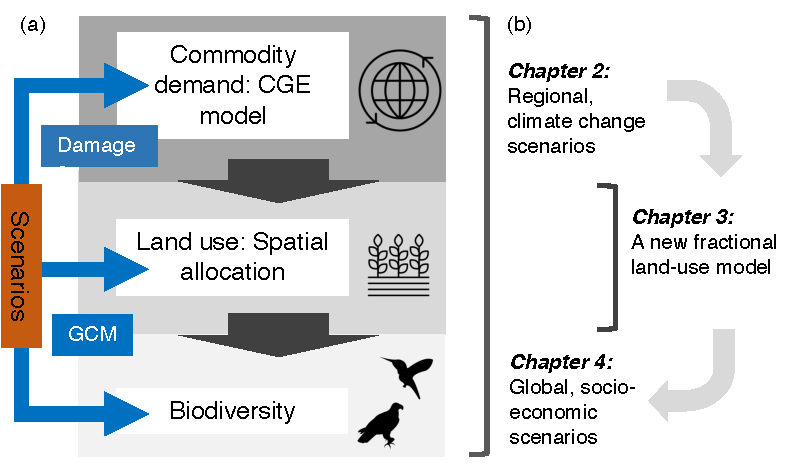
\includegraphics{chapters/figures/chapter1/fig_structure.pdf}
    \caption{Structure of this thesis in terms of the set-up of our framework. (a) Our modelling framework applying Computable General Equilibrium (CGE) models to predict commodity demand, land-use models to spatially downscale these demands and biodiversity models to predict biodiversity outcomes. Throughout our framework, scenarios have been parametrized through economic damages and general circulation models (GCM). (b) Thesis chapters in terms of the framework. Chapter 2 provides a first, regional implementation of our integrated assessment framework in which climate change impacts (RCP) are parametrized. Chapter 3 specifies a new fractional land-use model to improve the linkage of macro-economic and biodiversity models. Chapter 4 provides a first global implementation of our framework in which the new land-use model is first applied to spatially downscale SSP and predictions are compared to those made by an existing IAM. Adapted from \citet{kapitza_assessing_2021}.}
    \label{ch4:fig_structure}
\end{figure*}

\section{Chapter outline}

\subsection*{\Cref{ch2}: Assessing biophysical and socio-economic impacts of climate change on regional avian biodiversity}

The second chapter provides the initial development and application of our integrated assessment framework to quantify the relative influence of direct biophysical and indirect socio-economic (via commodity demand and land-use change) climate change impacts on bird species in Vietnam and Australia. In this chapter, we spatially downscaled projected changes in commodity demand using an existing categorical land-use model with limited applicability at global, fine-resolution extents.

\subsection*{\Cref{ch3}: A predictive model of fractional land use}
Resulting from \Cref{ch2}, we determined that in order to upscale our modelling framework to the global extent and align land-use predictions with the requirements posed by global-scale biodiversity modelling, it was necessary to develop a new fractional land-use model. In chapter 3 we introduce and validate a new land-use model to interface global commodity demand projections and biodiversity change. The model enables fine-scale mapping of future land-use under alternative scenarios of commodity demand change. It represents land-use as fractional cover within grid cells, thus providing higher information content than discrete categories of land-use without the need to decrease the spatial resolution.

\subsection*{\Cref{ch4}: Toward streamlined and transparent economic-ecological predictions of land-use change impacts on biodiversity}

Building on the methods and knowledge generated from \Cref{ch2,ch3}, \Cref{ch4} presents a first global implementation of our framework to predict global biodiversity under baseline SSP, thus paving the way for further analyses of climate change mitigation and adaptation scenarios on biodiversity. In this chapter, we parametrize baseline SSP in our CGE model and use the land-use model developed in \Cref{ch3} to spatially downscale commodity demand change expected under SSP2 and SSP5. We also further extend our land-use model by implementing a method to predict land-use intensity. We apply biodiversity models to project biodiversity intactness. We compare land-use and biodiversity predictions made using our framework with those made using an existing ingegrated assessment model and demonstrate that our streamlined, simplified modelling framework provides a robust means to predict biodiversity change without the high parametrization requirements of existing integrated assessment frameworks.

\subsection*{\Cref{ch5}: General discussion}

This chapter provides synthesis of the main findings of the thesis and relates them to the thesis aims. It evaluates the developed methods in terms of their transferability to other study contexts. Future research potentials are highlighted.

\subsection*{Appendices}

\Cref{apx:ch2,apx:ch3,apx:ch4} contain all supplementary information for \Cref{ch2,ch3,ch4}. \Cref{apx:ch5} contains links to all \texttt{R} scripts written for this thesis and information about developed packages.

\chapter{Assessing biophysical and socio-economic impacts of climate change on regional avian biodiversity}\label{ch2}
\newpage

{\parindent0pt
\textbf{SCIENTIFIC REPORTS}

\vspace{2cm}

\textbf{Article title}: Assessing biophysical and socio-economic impacts of climate change on regional avian biodiversity

\vspace{1cm}

\textbf{Authors}: Simon Kapitza\textsuperscript{1*}, Pham Van Ha\textsuperscript{2}, Tom Kompas\textsuperscript{2,3}, Nick Golding\textsuperscript{1}, Natasha C. R. Cadenhead\textsuperscript{1,4}, Payal Bal\textsuperscript{1} and Brendan A. Wintle\textsuperscript{1,4}

\vspace{1cm}

\textbf{Author affiliations}:

1 Quantitative and Applied Ecology Group, School of BioSciences, The University of Melbourne, Parkville, Victoria, 3010, Australia

2 Crawford School of Public Policy, Lennox Crossing, Australian National University, Australian Capital Territory, 2601, Australia

3 Centre of Excellence for Biosecurity Risk Analysis, School of BioSciences, The University of Melbourne, Parkville, Victoria, 3010, Australia

4 NESP Threatened Species Recovery Hub, University of Melbourne and University of Queensland, St Lucia, Queensland, 4072, Australia

\vspace{1cm}

Length abstract: 150

\vspace{1cm}

Length manuscript: 5134

\vspace{1cm}

Display items: 4

\vspace{1cm}

References: 77

\vspace{1cm}

Corresponding author: Simon Kapitza, Quantitative and Applied Ecology Group, School of BioSciences, The University of Melbourne, Victoria, 3010, Australia, simon.kapitza.research@gmail.com
}

\pagebreak

\section{Abstract}

Climate change threatens biodiversity directly by influencing biophysical variables that drive species’ geographic distributions and indirectly through socio-economic changes that influence land use patterns, driven by global consumption, production and climate. To date, no detailed analyses have been produced that assess the relative importance of, or interaction between, these direct and indirect climate change impacts on biodiversity at large scales. Here, we apply a new integrated modelling framework to quantify the relative influence of biophysical and socio-economically mediated impacts on avian species in Vietnam and Australia and we find that socio-economically mediated impacts on suitable ranges are largely outweighed by biophysical impacts. However, by translating economic futures and shocks into spatially explicit predictions of biodiversity change, we now have the power to analyse in a consistent way outcomes for nature and people of any change to policy, regulation, trading conditions or consumption trend at any scale from sub-national to global.

\section{Introduction}
Climate change affects biodiversity through a multitude of pathways. There is pervasive evidence that climate change directly affects environmental conditions that are related to the climatic niches of many taxa, with the potential of significant shifts in their distributional ranges or even the total extinction of species \citep{ipbes_summary_2019, struebig_targeted_2015}. However, climate change also affects biodiversity through indirect human-mediated impacts: it drives the loss of livelihoods and displacement \citep{mcmichael_climate_2006} and affects food and commodity production systems through its impacts on land productivity and human health\citep{roson_estimation_2016, tol_who_2014} and environmental suitability for different land uses \citep{veldkamp_clue_1996, verburg_combining_2009}. Resulting global transitions of land use patterns are set to drive habitat conversion and may have dramatic impacts on biodiversity \citep{mantyka-pringle_climate_2015,oliver_interactions_2014, newbold2019climate}. While there are some examples of studies examining synergistic effects of land use and climate change on species \citep{brodie_synergistic_2016, brambilla_climate_2016}, large-scale assessments of biodiversity change in response to climate change have tended to look only at direct impacts of climate change on biophysical conditions or habitat loss and fragmentation alone8. Analyses that couple direct biophysical impacts on species with indirect socio-economic impacts via consumption, commodity, and land use change are sorely needed to fill important gaps in our knowledge of interactions between land use and climate change \citep{newbold2019climate}, to foster a more holistic understanding of the impacts of climate change, and to support the design of cross-sectoral adaptation and mitigation strategies \citep{ipbes_summary_2016}.

No single model of drivers of change in biodiversity and ecosystem services can capture all relevant dynamics at a high level of detail and there is an increasing awareness of the urgency to consider interactions between direct and indirect drivers of change under future scenarios to characterise prospects and management options for biodiversity and ecosystem services \citep{ipbes_summary_2016}. Coupling demographic, economic and biophysical models has the potential to advance understanding and improve representation of synergies between direct and indirect drivers in biodiversity modelling, and to discover non-linear system behaviours that may not be apparent when considering drivers in isolation \citep{ipbes_summary_2016}.

Here, we contribute to the recent advances in integrated assessment modelling \citep{leclere_bending_2020,  newbold_future_2018, powers_global_2019, marques_increasing_2019} by applying an integrated modelling framework to compare the relative influence of direct biophysical and indirect socio-economic climate change impacts on the distribution and extent of suitable ranges for avian species in Vietnam and Australia (\Cref{ch2:fig1}).

\begin{figure*}[htb]
  \centering
  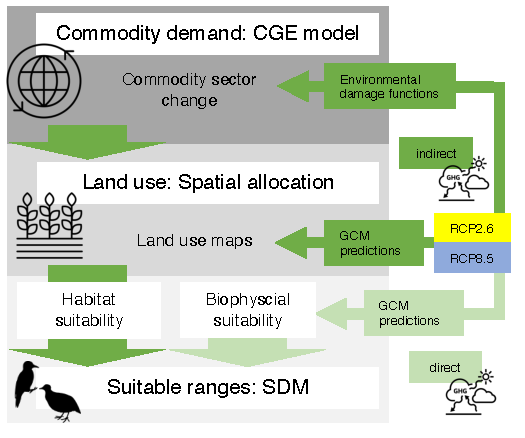
\includegraphics[width=0.7\textwidth]{chapters/figures/chapter2/fig1.pdf}
  \caption{Overview of the modelling framework to capture interactions between direct and indirect drivers of biodiversity change under climate change scenarios. We included two Representative Concentration pathways RCP2.6 and RCP8.5 to characterize the plausible extremes of climate change. Dark green arrows represent the indirect pathway of climate change impacts on suitable ranges. Light green arrows indicate the direct pathway of climate change impacts on ecological suitability. Icons from thenounproject.com.}
  \label{ch2:fig1}
\end{figure*}

Recent advances in computable general equilibrium (CGE) modelling \citep{van_ha_building_2017, van_ha_solving_2016} bring unprecedented power to parametrise the impacts of climate change on commodity consumption and production patterns at very high commodity and temporal resolution across the global economy. We combine this economic modelling power with state-of-the-art land use change modelling to spatially downscale commodity demand changes caused by climate change \citep{roson_estimation_2016} into changes of land use patterns. In order to isolate net climate change impacts on the economy, we parametrize only climate change damages in the CGE model, keeping all other economic parameters constant at current baseline values. The spatial realisation of changing land use patterns varies with changes in the suitability of land for particular uses and is thereby also driven by climate change \citep{verburg_combining_2009, fuchs_high-resolution_2013}. Commodity demand changes are projected annually and land use predicted in 10-year time steps, producing decadal time-series maps of land use. Maps are integrated with climate change predictions into a biodiversity impact assessment using species distribution models (SDMs) \citep{lawson_prevalence_2014, wintle_fauna_2005, wintle_ecologicaleconomic_2011, thomas_climate_2004}. SDMs, fitted to current climate, land use, and other environmental variables (\Cref{apx:ch2:tab1}) are extrapolated to conditions in 2070 under a range of climate and land use scenarios. Predictions of relative likelihood of occurrence are thresholded to examine changes in the ecologically suitable ranges for 1282 bird species in Vietnam and Australia \citep{lawson_prevalence_2014, wintle_fauna_2005, wintle_ecologicaleconomic_2011, thomas_climate_2004}.

\section{Results}
\subsection{Direct biophysical impacts dominate changing range sizes.}

\begin{figure*}[htb]
  \centering
  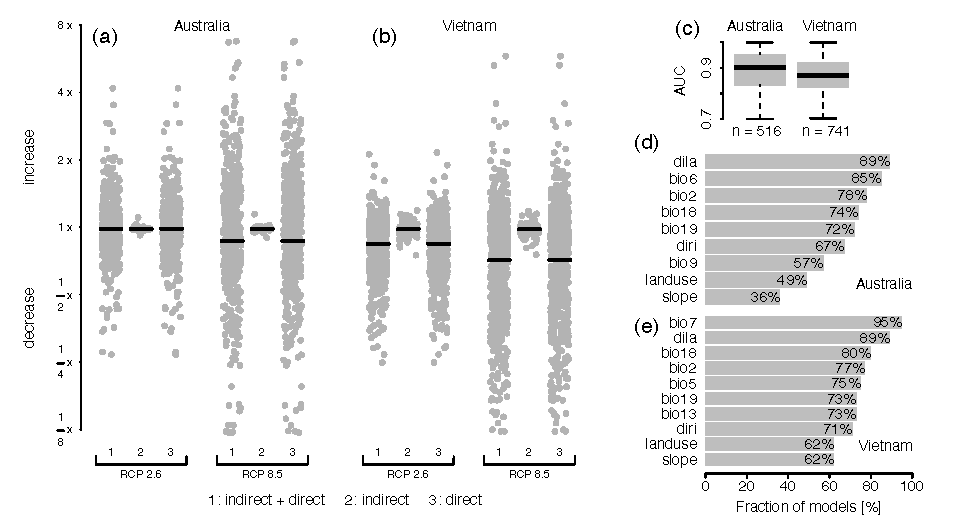
\includegraphics[width=\textwidth]{chapters/figures/chapter2/fig2.pdf}
  \caption{Predicted changes in species’ ecologically suitable ranges. (a, b) Illustration of multiplicative changes in species’ ecologically suitable ranges between present (2018) and 2070 for Australia and Vietnam respectively, under three treatments (1) “indirect + direct” (combined biophysical and socio-economic impacts of climate change), (2) “indirect” (net socio-economic impacts) and (3) “direct” (net biophysical impacts). Each point corresponds to a species, black bars are means of ecologically suitable range changes across all species. (c) A summary of cross-validated test Area Under the Receiver Operating Characteristics Curve values (AUCs) \citep{jimenez-valverde_insights_2012} of models in the two regions as well as the respective number of models (n) retained (AUC $>$ 0.7) \citep{baldwin_use_2009}. AUC provides a measure of a model’s discriminatory performance in terms of how well test predictions discriminate between occupied and unoccupied locations \citep{jimenez-valverde_insights_2012, baldwin_use_2009}. (d, e) Fractions of models in which a predictor was used. Full names and definitions of all predictors can be found in \Cref{apx:ch2:tab1}. Figure created in \texttt{R} version 3.5.176 (https://www.R-project.org/).}
  \label{ch2:fig2}
\end{figure*}

For birds in both regions, we forecast major declines in ecologically suitable ranges, with severity of loss scaling with the severity of climate change (\Cref{ch2:fig2}). Under RCP 8.5, a much higher number of species would be expected to experience decreases of more than half of their present ecologically suitable range compared with RCP 2.6, although variation in responses is also greater, indicated by the much wider spread of points (\Cref{ch2:fig2}a,b). In Australia, mean suitable range decline under both pathways is not predicted to be as severe as in Vietnam and a smaller number of species is predicted to lose more than half of their suitable range. For both Vietnamese and Australian birds, predicting only under the indirect (land use change) effects of climate change results in little change to mean predicted outcomes for species (\Cref{ch2:fig2}a,b), though some threatened species are predicted to lose significant suitable range within their current range due to indirect climate change impacts (see below). However, our analysis focuses on net climate change impacts on the economy; species ranges are likely to be affected more severely when also parametrizing other economic parameters to reflect future economic change. Mean predictions under combined direct and indirect effects do not differ to any notable degree from those made under direct biophysical effects only. Predictions under the first and third quartiles of bioclimatic variables across 15 Global Circulation Models (GCMs) show the same trends identified in the main results (\Cref{apx:ch2:fig1}).

SDMs for 1436 bird species were used in the analysis of the direct and indirect impacts of climate change on biodiversity. Discriminatory performance of the SDMs was assessed using cross-validated AUCs which varied between 0.7 and 1.0 with a mean of 0.90 in Vietnam and 0.87 in Australia (\Cref{ch2:fig2}c), indicating very high discriminatory performance. We discarded models for 179 species with AUC $<$ 0.7 (see Methods). The predictor variables retained in the highest fraction of models were distance to lakes (dist lakes) in Australia and annual temperature range (\textit{bio7}) in Vietnam. These are followed by dist lakes and precipitation of warmest quarter (\textit{bio18}) in Vietnam, and by minimum temperature of the coldest week (\textit{bio6}) and mean diurnal temperature range (\textit{bio2}) in Australia. In Australia, land use was retained in about half the models. The very minor indirect (via land use) impact predictions arise because the changes in commodity demand predicted by the CGE model did not result in significant changes to land use in both regions (see below).

\subsection{Land use changes in response to climate change vary by region.}
The total output of most agricultural crop sectors in both regions was predicted to decrease more with increasing climate change. In particular, in Vietnam, sectors such as oil seeds and plant-based fibres shrink by up to 20\% under RCP 8.5 (\Cref{ch2:fig3}a). The land requirements for each sector generally increase in proportion to the overall output of each sector. This is due to climate change impacts on crop yields as parametrised in the CGE-model: reductions in land productivity mean that more land is required to maintain sector outputs. Accordingly, in both countries, even while total outputs tend to decrease, land requirements of agricultural sectors remain approximately the same, or increase slightly (\Cref{ch2:fig3}a).

\begin{figure*}[htb]
  \centering
  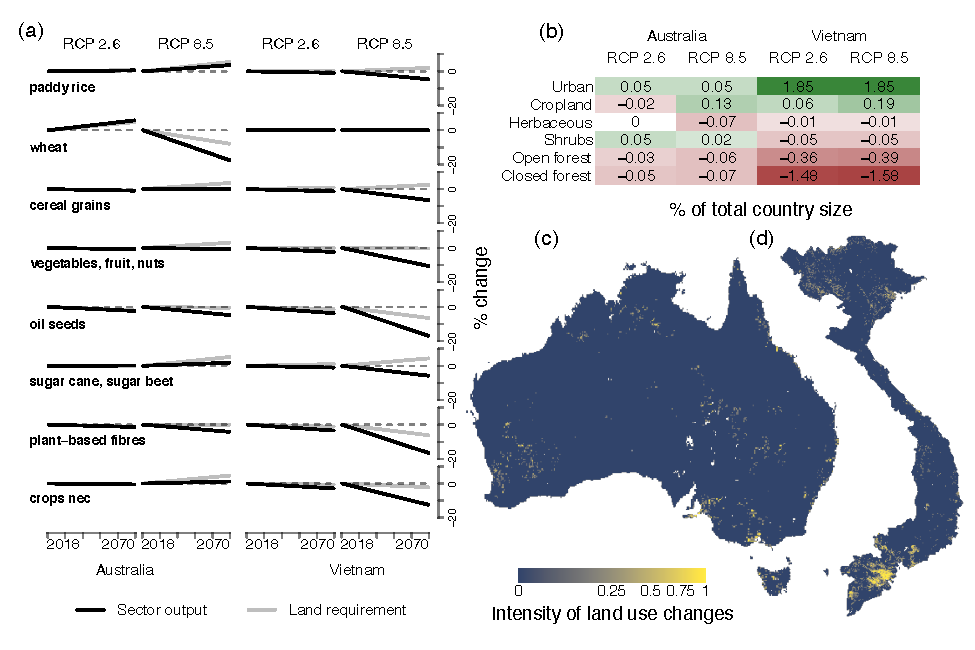
\includegraphics[width=\textwidth]{chapters/figures/chapter2/fig3.pdf}
  \caption{CGE and land use model results. (a) Future projections of commodity sector output and sector land endowments (the area required to produce output of a sector) from CGE model under RCP 2.6 and RCP 8.5. (b), Illustration of the percentage change of each land use in response to GTAP projections of crop sectors in a and FAO urban population projections, grouped by country and RCP, relative to the whole country size. (c-d) Intensity of predicted land use changes under indirect effects of RCP 8.5 in (c) Australia and (d) Vietnam. These maps are derived by aggregating predicted land use changes between any two classes under the indirect impacts of RCP 8.5 by factor 3.  Figure created in \texttt{R} version 3.5.1 (https://www.R-project.org/) \citep{r_development_core_team_r_2008}.}
  \label{ch2:fig3}
\end{figure*}

The changes in land requirements for crop lead to an increase in cropland of $<$ 0.5\% of the total land area in both regions under RCP 8.5 and a very slight decrease in Australia under RCP 2.6 (\Cref{ch2:fig3}b). Increases in urban land in both countries were modelled on FAOSTAT estimates of urban population growth \citep{fao_faostat_2017}. In Australia, land use changes occur locally and are concentrated in coastal areas along the north-east, south and west of the continent, although some changes also occur further inland (\Cref{ch2:fig3}c). In Vietnam, land use change is higher overall, with a particular concentration of change in the central-southern and northern coastal areas of the country, that also approximately coincide with the country’s major river deltas (\Cref{ch2:fig3}d). Given that the distributions of most species are constrained, aggregated, and not random, small percentage changes in land use at the national scale still have significant impacts on some species locally (\Cref{ch2:fig4}a, c). For example, species losing more than 10\% of their currently suitable range under indirect impacts of RCP 8.5 in Vietnam include the vulnerable chestnut-necklaced partridge (\textit{Arborophila charltonii}) and the near-threatened yellow-billed nuthatch (\textit{Sitta solangiae}). These declines are highly localised and predominantly occur in the centre-south of the country (\Cref{ch2:fig4}c). Direct climate change impacts are more severe: 324 and 362 species lose at least 10\% of their suitable ranges under direct impacts of RCP 2.6 and RCP 8.5 respectively, with areas particularly affected across taxa under RCP 8.5 in the northern highlands and the central eastern parts of the country (\Cref{ch2:fig4}d). Among the species losing more than 95\% of their current suitable range under the direct impacts of RCP 8.5 are the Chinese thrush (\textit{Turdus mupinensis}) and the critically endangered white-rumped vulture (\textit{Gyps bengalensis}) (\Cref{ch2:fig4}c, d).

In Australia, no species was found to lose more than 10\% of its currently suitable range under indirect climate change impacts, although the black-throated whipbird (\textit{Psophodes nigrogularis}) loses more than 5\%. A higher number of species are affected by the direct impacts of climate change, with areas predicted to suffer particularly high suitable range declines along the southern and eastern coasts, the southwest and the southeast of the continent. In Australia, 188 and 230 species are expected to lose more than 10\% of their suitable range under RCP 2.5 and RCP 8.5 respectively.

Amongst the Australian species losing more than 95\% of their suitable range under the direct impacts of RCP 8.5 are the kalkadoon grasswren (\textit{Amytornis ballarae}) and the Australasian pitpit (\textit{Anthus Australis}) and a number of other species now categorised as of least concern (\Cref{ch2:fig4}b). This highlights the potential dangers of climate change to species that we do not yet consider under threat, but for which extinction debts are accruing \citep{kuussaari_extinction_2009}.

\begin{figure*}[htb]
  \centering
  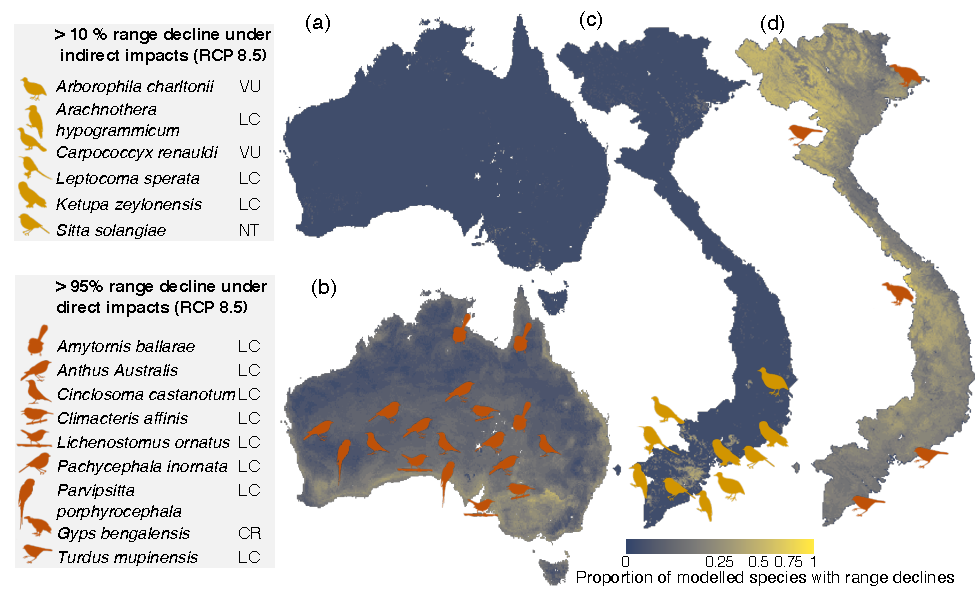
\includegraphics[width=\textwidth]{chapters/figures/chapter2/fig4.pdf}
  \caption{Mapping of habitat loss under RCP 8.5. (a–d),  The proportion of avian species predicted to lose ecologically suitable range across Australia (a, b) and Vietnam (c, d) under the indirect (a, c) and direct (b, d) climate change impacts under RCP 8.5. Cell shading indicates the proportion of species predicted to lose suitable range in each cell.  This identifies areas of declines in species’ suitable ranges from either indirect or direct impacts. The icons indicate locations of suitable range declines for severely affected species that lose more than 10\% (indirect) and more than 95\% (direct) of their suitable ranges overall. IUCN conservation status is given alongside taxonomic names (LC – least concern; VU – vulnerable; NT – near threatened; EN – endangered; CR – critically endangered) \citep{iucn_iucn_2018}. Icon credit - http://phylopic.org.  Maps created in \texttt{R} version 3.5.1 (https://www.R-project.org/) \citep{r_development_core_team_r_2008}.}
  \label{ch2:fig4}
\end{figure*}

The expected direct impacts of climate change impacts on many taxa are well researched and documented (i.e. increased extinction risks across taxa with accelerated climate change \citep{urban_accelerating_2015}, northward shifts of bird distributions in Great Britain under climate change \citep{gillings_directionality_2015} and responses of bird abundance to climate change in the United States and Europe \citep{stephens_consistent_2016}). Our findings largely agree with these trends. In both Australia and Vietnam, climate change is likely to have extensive detrimental impacts on the climatically suitable ranges of birds. For many species, suitable ranges decline with increasing severity of climate change (\Cref{ch2:fig2}) and under RCP 8.5, 24\% of species analysed (in Vietnam) show likely declines in suitable ranges of greater than 50\%, increasing their extinction risk in the country severely. Our analysis shows that subject to the assumptions of this work, the relative contribution of direct, biophysical impacts of climate change on biophysical suitability in our study area outweighs the contribution of indirect socio-economic impacts on habitat suitability via global commodity markets and resulting land use change, also taking into account the fact that climate change impacts on the suitability of land for particular uses. In Vietnam and Australia, bird species appear to be more severely impacted by the direct influence of changing climates than by its indirect impacts via commodity demand and land use.

\section{Discussion}

Better understanding of climate change impacts on commodity demand and supply, and how those changes impact biodiversity should remain a research priority.
We predict economic change under two climate change scenarios, keeping all other aspects of the global economy at current baseline values. This way, we could capture and isolate the effect of climate change on the economy. However, this approach omits other socio-economic processes that could affect supply and demand, such as population growth, changes to economic growth, energy efficiency, and shifts in social demands. These other factors may impact habitat and biodiversity through agricultural expansion, deforestation or urbanisation. While this study was designed to assess the net effects of direct and indirect climate change impacts on species as a first case study introducing our integrated assessment framework, these factors will be incorporated in future iterations that include an even more comprehensive CGE parametrization (i.e. full CGE baseline scenarios with socio-economic pathway narratives \citep{van_vuuren_climate_2014} and integration of climate models in CGE analysis) and through improvements to current CGE methods by including, for example, stochastic effects of natural disasters in the CGE modelling.

Our results are valid for avian taxa in Australia and Vietnam under a number of assumptions about how commodity demand and supply, land use and biodiversity interact to deliver outcomes predicted by our integrated model. In our assessment framework, we follow a top-down modelling approach; within the architecture of our CGE model, climate change affects global demand and supply of many land-based commodities, requiring sector outputs as well as requirements of land to each sector to increase or decrease. However, mapped land use changes corresponding to changes in land endowments to different commodity sectors do not feed back into the CGE model. The inclusion of such feedbacks would increase the realism of both CGE and land use predictions, but detailed knowledge of local production systems and commodity markets are required to accurately parameterise such a model, and such models are computationally expensive \citep{bryan_land-use_2016}.

We chose not to produce SDMs for species with less than 20 occurrence records, to avoid the inflation of AUC for range-restricted species and species with very low prevalence \citep{van_proosdij_minimum_2016} and to assure sufficient discrimination between presences and background points \citep{hernandez_effect_2006, wisz_effects_2008}. Rare or spatially restricted species can be more vulnerable to localised impacts such as habitat loss38, but these effects are difficult to capture when biodiversity data are poor. We assumed unlimited dispersal ability in Vietnam and dispersal ability constrained to bioregions adjacent to those containing observation records in Australia. Disconnected patches of potential habitat outside of observed ranges (but within adjacent bioregions in Australia) were counted in future predictions, regardless of whether those areas were functionally linked (by suitable or traversable habitats) to the observed range and thus within the dispersal range of species. This may lead to an over-estimation of habitat utilisation and a commensurate underestimation of both direct and indirect impacts of climate change, particularly for taxa with a low dispersal ability that rely on small pockets of habitat within their range and are unable to reach disconnected patches of potential habitat. The importance of connectivity as a key component of habitat structure is well known39 and crucial for population viability in many species with low dispersal ability \citep{gordon_use_2012, cadenhead_climate_2016}. The parametrization of species’ dispersal ability and explicit modelling of landscape structure in response to land use change would allow for the inclusion of these fragmentation effects. This may be particularly important when our framework is extended to non-avian species.

While we found that total agricultural sector outputs decrease in both Vietnam and Australia, decreases in land productivity mean that land use in production for some agricultural commodities were predicted to increase slightly. We assumed a global economic equilibrium in which commodities can be substituted through trade between regions, thus implying that global demand for land-based commodities is serviced by regions that benefit from a comparative advantage under climate change. Where comparative advantage is due to increases in land productivity (land use efficiency), additional land may not be required to increase outputs. However, where this advantage is due to other economic mechanisms and not driven by the cost of converting additional land for production, more land may be allocated to agricultural or other commodity production, increasing habitat loss. For example, in Canada, our CGE model predicted an increase of wheat sector output by over 37\% under RCP 8.5, while land endowments increase by only 14\% due to increases in land use efficiency. In India, wheat output is estimated to increase by 8\% under RCP 8.5, while land endowments to the wheat sector increase by 6\%, suggesting much lower land use efficiency in India than in Canada (see \Cref{apx:ch2:fig2} for a global, country-wise mapping of projected changes in sector outputs and land endowments of the wheat sector). Despite lower land use efficiency, wheat production in India still grows, because growth is economically feasible as long as it is not limited by factors arising from the sector’s context in domestic and international markets. In both countries, increases in land use lead to agricultural expansion, but in Canada more wheat can be produced per unit land and areas lost to wheat farming are likely to be much smaller per produced unit than in India. Nonetheless, if wheat production occurs in parts of Canada that were previously in, for example, natural prairie, then significant biodiversity losses may occur. Our framework provides in-depth insight into the links between sectors and regions and allows for a better understanding of global shifts in land requirements, enabling the fine-scale identification of hotspots for production, agricultural expansion and ultimately habitat destruction under consideration of the global economic processes.

In this first implementation of our framework we could capture and quantify principal relationships between climate change, the global economy, land use and avian habitat. Future uses of our approach could include regional and global biodiversity assessments following individual policy shocks, such as the introduction or abolishment of taxes or international trade deals, or could seek to capitalize on existing narratives of socio-economic futures and climate change pathways (so-called Shared Socio-economic Pathways) \citep{van_vuuren_climate_2014} to parametrise climate adaptation policies, sustainable development goals and other aspects of socio-political transitions within the CGE modelling. Expanding consideration of biodiversity to include non-avian taxa and explicitly dealing with the role of connectivity and dispersal will enable a more comprehensive assessment of biodiversity impacts under socio-economic change. A key feature of our approach is that it provides opportunity to downscale country-level commodity demands to spatial explicit land use changes and biodiversity impacts, enabling a more meaningful analysis of the habitat and biodiversity implications of economic shocks or the implications of trade than have previously been possible. 

Better integration of models and scenarios of biodiversity is required to guide evidence-based climate adaptation strategies and to chart progress toward sustainable development goals43. Our approach to integrating economic, land use and biodiversity values into a single model capable of high resolution, spatially-explicit predictions of land use and biodiversity outcomes provides information in a form that can be used directly by planners and managers. While spatial predictions of biodiversity and land use change have been available for decades, being able to place these predictions coherently in a global economic context is a new and exciting development that will bring a new level of relevance and realism to predictions in the eyes of policy and decision makers.

\section{Methods}
\subsection{Study area} 
We focussed our analysis on Vietnam and Australia because the countries provide unique socio-economic contexts, while hosting a similar number of bird species that are vulnerable, endangered or critically endangered \citep{birdlife_international_country_2018, birdlife_international_country_2018-1}. SDMs for Vietnam were built using data from a 30 x 30-degree tile that comprises large parts of Southeast Asia. This enabled us to capture the occurrence of bird species present in Vietnam on larger environmental gradients.

\subsection{Climate Change} 
We chose Representative Concentration Pathways RCP2.6 and RCP8.5 \citep{van_vuuren_representative_2011} to include two extremes of the expected radiative forcing levels. For each pathway, we acquired the 2070 predictions of 19 bioclimatic variables47 from 15 GCM of Coupled Model Intercomparison Phase 5 (CMIP5) \citep{taylor_overview_2012}. To capture variation between GCM predictions, we determined the cell-wise first, second and third quartiles each of the 19 variables across the 15 GCM (\Cref{apx:ch2:tab2}).

Main results were derived by predicting land use and species distributions under the medians of these variables. We predicted both land use and species distributions under the first and third quartiles to approximate the range of outcomes for species across all 15 GCM (\Cref{apx:ch2:fig1}). In CGE models, we included the parametrization of both climate change pathways proposed by \citet{roson_estimation_2016}.

\subsection{CGE models} 
We developed an inter-temporal Global Trade and Analysis Project (GTAP) model \citep{hertel_global_1997} to simulate changes in production under different climate change scenarios. CGE models use input-output-tables derived from national economic census data. These tables represent the inputs required in each economic sector to produce outputs and meet household and government demands (both nationally and internationally), which in turn are affected by prices and thus supply. Sectors are linked within each national economy, but also between economies. Producers in each country can produce various commodities to sell to domestic or foreign households and governments. Households and governments generate their income from selling (to producers) productive input factors (land, capital, labour, etc.) and through taxes. In our version of GTAP, the total land area (land endowment) from which allocations are made to crop sectors (land requirements) can be changed in the baseline. Therefore, land supply is not necessarily fixed, as is the case in most other GTAP models.  
Estimations within GTAP are carried out relative to this baseline supply and we convert relative changes in agricultural land requirements to absolute changes in cropland by using their respective shares in the total harvested area for a by-sector-weighting of the average relative change of all classes (\Cref{apx:ch2:tab3}). This weighted average change is applied on the current area under cropland to derive a future value. Accordingly, there is a direct proportional link between changes in land requirements and changes in the total area of agricultural land and the total area under agricultural land can change at the expense, or to the benefit, of other classes. 

Since our GTAP model is a general equilibrium model, any shock to productivity will affect both the demand and supply of an agricultural commodity. The marginal cost of production generally increases (with the loss of productivity). At the same time, the income of households in the model will also be affected by the change in productivity as incomes are derived from selling (or renting) productive factors (land, capital, labour, and natural resources). As a result, prices change to equalize demand and supply and a substitution effect between agricultural commodities and between agricultural and other commodities takes place. As a result, demand does not stay constant. The contraction or expansion of the production of a particular crop is a result of interaction between demand and supply for that crop (both domestically and internationally). 

Our inter-temporal GTAP model uses the GTAP 9 database 50, which is subdivided into 139 regions and 57 commodity sectors \citep{aguiar_overview_2016} and extends the GTAP model by replacing the recursive dynamic module of the current GTAP model with a forward-looking dynamic (or inter-temporal) module, where the producer can optimise profits overtime \citep{van_ha_building_2017, kompas_effects_2018}. The inter-temporal GTAP model allows optimal investment behaviours, in which producers in each country can adjust their decisions based on the impacts from both past and foreseeable future events. Agents in the model can react to future threats long before their full realisation \citep{kompas_effects_2018}. This makes the model a perfect tool for the simulation of future phenomena like climate change.

Following \citet{roson_estimation_2016}, climate change impacts in our GTAP model are realised as shocks to land supply and agricultural and labour productivity. The reduction in endowments of productive land and productivity negatively affect the production of commodities. Agricultural commodities are expected to be the most affected. With production shrinking more in some commodities than others, the price will adjust to balance the demand and supply of commodities. As a result, we will see a substitution effect between domestically produced products and their competitive imports along with a substitution effect in factors of production (such as land), balancing demands between sectors.
Unlike the \citet{kompas_effects_2018} approach, which relied on a one-step simulation approach, here we apply a multi-step simulation approach allowing the shocks to be applied into smaller successive intervals combined with extrapolation techniques to further enhance the simulation accuracy \citep[see]{horridge_gempack_2018,pearson_solving_1991} for the details on multi-steps CGE solution methods). The solution of the inter-temporal GTAP model in this paper has been carried out within a parallel computing platform \citep{van_ha_solving_2016, kompas_curse_2018} with the use of PETSC 56–58 and HSL 59 libraries.

\subsection{Land use models.} We reclassified a global land-use map to 8 land use classes (urban, cropland, herbaceous ground vegetation, shrubland, open canopy forest, closed canopy forest and wetlands and barren land) (\Cref{apx:ch2:tab1} for a full list of data sources). Changes in urban land were estimated using estimates of urban population changes \citep{world_bank_group_population_2016} and adjusting the amount of land under this class, assuming that urban population density remains steady through time. Future applications of this work will establish links between land-use classes related to forestry and livestock-raising, as has been demonstrated recently \citep{marques_increasing_2019}.

We predicted land use maps under both pathways in 10-year time steps, using an \texttt{R} implementation \citep[\texttt{R} package \texttt{lulcc}]{moulds_open_2015} of the Conversion of Land Use and its Effects at Small regional extents (CLUE-S) model by \citet{verburg_modeling_2002}. First, we determined the local suitability for different land uses through logistic regression of land use against the linear combination of a range of biophysical and socio-economic drivers in Generalised Linear Models (GLMs), from 15,000 randomly sampled pixels in each region (\Cref{apx:ch2:tab1}) for a detailed list of data, \Cref{apx:ch2:fig3} for effect sizes of predictors in each GLM). The selection of variables for land use suitability models was based on work by \citet{verburg_land_1999}. Correlation analysis eliminated highly correlated predictor pairs (Spearmen's rank correlation coefficient \(\geq 0.7\)), always keeping the predictor whose highest correlation with any other remaining predictor was smaller, to maximise independent information retained in the final set. The final predictor sets were checked against literature \citep{verburg_downscaling_2006, verburg_spatial_1999}. We discarded a small number of predictors using cross-validated Lasso penalisation in the \texttt{glmnet} \texttt{R}-package \citep{friedman_regularization_2010} and used the reduced predictor sets to build GLM and predict to future timesteps by interpolating GCM-predicted WorldClim variables (\Cref{apx:ch2:tab2} for used GCM). GLM predictions produced maps of the landscape's potential suitability for each land use class. Transitions between classes were constrained through a matrix detailing possible transitions (\Cref{apx:ch2:tab4}). We specified conversion elasticities of each class (total possible turn-over within each class) based on literature \citep{moulds_open_2015,verburg_modeling_2002}.

Projected demand changes were allocated iteratively until estimated land area demands were met \citep{fuchs_high-resolution_2013}. Competition between land uses is handled in CLUE-S by allocating the land-use with the highest predicted suitability in a given cell, accounting for conversion elasticity and allowed transitions. We masked category I and II protected areas \citep{iucn_world_2014}, precluding these areas from land-use changes. Since there was no CGE-modelled future demand for herbaceous ground vegetation and shrubland, as well as the forest classes, the overall amount of area allocated to those land uses was what was not allocated to satisfy projected agricultural and urban demands. The proportional allocation between each of these residual classes was determined based on their mean predicted suitability in the landscape.

Species distribution models. Correlative species distribution models (SDM) can predict responses of species to changing environmental conditions by extrapolating from the covariate space in which they were observed \citep{lawson_prevalence_2014, wintle_fauna_2005, wintle_ecologicaleconomic_2011, thomas_climate_2004}. The MaxEnt software package \citep{phillips_internet_nodate} (ver. 3.3.3k) was used to fit SDMs for 656 bird species in Australia and 739 bird species in Vietnam, using presenc-only data from the Global Biodiversity Information Facility \citep{gbif_gbif_2016}. We filtered records to retain observations from 1950-2018 with more than or equal to 20 occurrence points. We included a range of biophysical, topographic and socio-economic predictors as well as land use (\Cref{apx:ch2:tab1}). Correlation analysis eliminated highly correlated predictors (see above). Literature review ensured that final predictor sets were ecologically meaningful to avian species across taxa \citep{gillings_directionality_2015, goetz_relative_2014, maggini_assessing_2014, coxen_species_2017} at our aspired scale. We kept 9 predictors for Australia and 10 predictors for Vietnam, including 5 and 6 climate predictors respectively. 

Sampling bias is a pervasive issue particularly affecting presence-only data that is often sampled opportunistically. We estimated sampling effort in response to demographic and topographic predictors \citep{stolar_accounting_2015} (\Cref{apx:ch2:tab1}). By selecting background points proportional to sampling effort, the its effect on the location of presence records is largely eliminated as a form of bias \citep{phillips_sample_2009}.

Predictions were made using the estimated quartiles and medians of bioclimatic variables and the according land use maps that were also predicted under quartiles and medians. We controlled overfitting by dropping predictors with a permutation importance  $<$ 1\%. Test AUC were estimated via 5-fold cross-validation of each model and final models built on all available records. Species for which only uninformative models were fitted (AUC $<$ 0.7) were excluded \citep{baldwin_use_2009}.

We recorded the log ratio of the respective number of cells with relative likelihoods predicted above MaxEnt's MaxSSS threshold \citep{liu_selection_2016} (where the sum of model sensitivity and specificity is maximised) between present (2018) and future time step (2070) as a measure of change. In Australia, we constrained this change estimation for each species to bioregions containing records of the species, and adjacent bioregions \citep{moran-ordonez_evaluating_2016}.

\subsection{Software and data}

All data preparation and modelling for land use and SDMs was conducted in \texttt{R} (version 3.5.1) \citep{r_development_core_team_r_2008}, using packages \texttt{lulcc} \citep{moulds_open_2015} for land use simulations and \texttt{dismo} \citep{hijmans_package_2011} for MaxEnt \citep{phillips_internet_nodate} models. All analyses and spatial predictions of the land use model and SDM were performed at 0.5 arc-minute resolution; approximately 1 km at the equator. SDM building and predictions were computationally expensive and required up to 50 GB of working memory on 12 parallel cores.

\section{Acknowledgements}
This work received funding under the Australian Research Council Discovery grant DP170104795. The authors acknowledge contributions made throughout the research phase by B. Bryan, P. Lentini, H. Kujala and J. Elith.

\section{Competing interests}
The authors declare no competing interests.

\section{Data and code availability}
Sources for data used in land use and species distribution modelling are listed in Supplementary Information. Direct download links to these data sets are available in the code repository accompanying this study (see below). We provide outputs of the CGE, land-use and species distribution models in a data repository (DOI: 10.26188/5ce25391e5b60). The GTAP database that underpins GGE modelling is available from GTAP under license. However, we provide input files and commented CGE modelling code that contains details of parameters settings for global economic models and detailed commodity demand output tables for each of the scenarios modelled upon publication. Components of the GTAP database can be provided on request. All \texttt{R}-code for land use and species distribution modelling is available online (DOI: 10.5281/zenodo.3517724). The tablo-code for the CGE modelling will be provided in the code repository accompanying this study upon publication.

\chapter{A predictive model of fractional land use}
\label{ch3}
\newpage

{\parindent0pt
\textbf{Title:} A predictive model of fractional land use

\vspace{1cm}

\textbf{Authorship:} Simon Kapitza\textsuperscript{1*}, Nick
Golding\textsuperscript{2,3}, \& Brendan A. Wintle\textsuperscript{1}

\vspace{1cm}

\emph{\textsuperscript{1} School of Biosciences, The University of
Melbourne, Parkville VIC 3010, Australia \newline \textsuperscript{2}
Telethon Kids Institute, Perth Children's Hospital, 15 Hospital Ave,
Nedlands WA 6009, Australia \newline \textsuperscript{3} Curtin
University, Kent St, Bentley WA 6102, Australia}


\vspace{1cm}

\textbf{Authorship contribution statement}

SK, BW conceived the idea of providing a fractional land use model. NG,
and SK and BW designed the model and validation steps. SK coded the
model and analyzed the data. SK led the manuscript with edits from NG
and BW.

\vspace{1cm}

\textbf{Data accessibility}

All input data required to repeat this work will be made available and
receive a permanent DOI through FigShare upon publication. An \texttt{R} package
containing the model source code is available on GitHub
(kapitzas/flutes). All code for data preprocessing and analysis is also
provided through a GitHub repository (kapitzas/frac\_lumodel). Both
repositories will be receive permanent DOI through Zenodo upon
publication.
}

\newpage

\section{Highlights}

\begin{itemize}
\item
  A model to predict fine-resolution fractional land use change, based
  on future land use demands.
\item
  Development version implemented as \texttt{R} package, making the model
  accessible to \texttt{R-}trained users.
\item
  Validation shows high prediction accuracy in Amazon basin, but the
  model can be fitted anywhere to predict future land use change.
\end{itemize}

\section{Abstract}

By mapping land use under projections of socio-economic change,
ecological changes can be predicted to inform conservation
decision-making. We present a land use model that enables the fine-scale
mapping of land use change under future scenarios. Its predictions can
be used as input to virtually all existing spatially-explicit ecological
models. Our model maps the fractional cover of land use within each grid
cell, providing higher information content than discrete classes at the
same spatial resolution. The method accurately reproduced land use
patterns observed in the Amazon, both in terms of the allocated
fractional amounts and also the direction of predicted land use changes.
A small case study showcases the application of our model to reproduce
patterns of agricultural expansion and natural habitat declines. The
model source code is provided as an open-source \texttt{R} package, making this
new method available to bridge the gap between socio-economic, land use
and biodiversity modelling.

\vspace{1cm}

\textbf{Keywords:} Land use forecasting, fractional land cover,
continuous fields, agricultural expansion, socio-economic change,
biodiversity conservation.

\section{Introduction}

Land use change is a key driver of global environmental change, causing
global declines in biodiversity, species extinctions and resulting in
the deterioration of ecosystem services
\citep{foley_global_2005, ipbes_summary_2019}.

Land use change is driven by bio-physical and socio-economic processes
\citep{lambin_global_2011}. Climate change will likely result in global
shifts and declines of land suitable for agricultural production, with
projected depletion of land reserves in the first half of the 21st
century \citep{lambin_global_2011}. Most socio-economic scenarios of
future change describe future increases in food production and
international trade of goods \citep{oneill_new_2014, oneill_roads_2017}.
Even under lowest impact scenarios, also known as `shared socio-economic
pathways' (SSPs), in which land use is strongly regulated, deforestation
rates are reduced, diets are more plant-based and climate change
mitigation starts early, crop and livestock production are still likely
to be higher and occupy a larger land area than they do today
\citep{oneill_new_2014}.

There is mounting evidence of adverse impacts of historic and current
land use change on biodiversity and the need for global assessments of
future biodiversity change in response to land use change has been
increasingly acknowledged
\citep{urban_improving_2016, kim_protocol_2018, powers_global_2019}.
However, work concerned with understanding future biodiversity change
tends to focus on climate change
\citep{titeux_biodiversity_2016, struebig_anticipated_2015, urban_improving_2016},
or other aggregated effects of socio-economic change, such as forest
loss \citep{perez-vega_comparing_2012, margono_primary_2014} and urban
expansion \citep{seto_global_2012}. Consequently, future predictions of
biodiversity change will benefit from explicit accounting of the drivers
and effects of land use change at the level of individual types of use.
Detailed, large-scale maps of future land use under competing future
scenarios provide useful insights for researchers and policy makers,
particularly in terms of informing conservation planning and preventing
future biodiversity loss.

Different conceptual approaches have found application in investigations
of past, present and future land use change. \citet{koomen_core_2011}
identify four theoretical core principles for modelling land use change.
Predictions can be made based on \emph{the continuation of historical
developments}, where past patterns are extrapolated into future
conditions, the \emph{suitability of land}, where land use changes are
predicted based on proximity to markets, biophysical conditions and
other environmental drivers, \emph{neighbourhood interactions}, where
neighbouring land uses affect local changes and \emph{actor
interactions}, where land use changes explicitly emerge from the
decision-making of individual actors, or groups of actors.

These principals appear in many existing models. For example, artificial
neural networks and markov chain models learn and infer patterns from
historic time series of land use change
\citep{tayyebi_modeling_2014, pijanowski_using_2002}. To allow for
spatially-explicit assessments, markov chain models have been frequently
combined with cellular automata \citep[CA-Markov models,
see][]{hyandye_markovian_2017, aburas_improving_2017, koomen_core_2011}.
In cellular automata the transition probability of a cell to another
land use depends on its current state and the state of neighbouring
cells, both of which are the result of historic changes
\citep{koomen_core_2011}. Cellular automata have been used successfully
to simulate strongly auto-correlated changes, such urban sprawl
\citep{verburg_land_2004, fang_impact_2005, shafizadeh_moghadam_spatiotemporal_2013, sun_modeling_2007}.

Some existing modelling approaches apply regression analysis and other
techniques to identify associations between various environmental
conditions and observed land use patterns
\citep{koomen_core_2011, lambin_global_2011, verburg_land_2004}. Available
models applying this approach include SLEUTH
\citep{dietzel_toward_2007}, DINAMICO EGO
\citep{soares-filho_modeling_2009}, IDRISI LCM
\citep{eastman_short_2018} and, perhaps most prominently, the Conversion
of Land Use and its Effects (CLUE) model series (\Cref{ch3:tab1}). CLUE models have found application in the
prediction of spatially-explicit patterns of land use at national and
continental scales
\citep{veldkamp_clue_1996, verburg_combining_2009, verburg_land_1999, verburg_modeling_2002, kapitza_assessing_2021}.
Exogenously determined future changes in area demands for different land
uses, often predicted by an economic model \citep{aguiar_overview_2016},
may be downscaled by establishing statistical relationships between
observed land use and a set of socio-economic and bio-physical drivers
of land use and land use change. Predicted land use suitability surfaces
inform local competition for different land uses
\citep{verburg_modeling_2002, meiyappan_spatial_2014}. Models can be
further parametrized by including transition rules at local (cell) and
landscape levels and constraints on overall turn-over through time. More
simplistic models based on statistical analysis use an ordered
allocation algorithm, in which competition between land uses is handled
by ordering allocations in terms of perceived socio-economic value
\citep{fuchs_high-resolution_2013}.

Most of these models apply statistical analyses of discrete land use
classes using binary logistic regression to model the cell-wise
probabilities of occurrence for each land use, independent of the
probabilities of other land uses. The resulting probability of land use
occurrence at a site produced by separate models is an incomplete
representation of the underlying structure of land use probability,
because it omits that occurrence probabilities are dependent between
land use types, and that the probabilities of all discrete classes must
sum to one. For example, when a site has very high probability for urban
land use, this implies relatively low probabilities for primary natural
habitat, which separate, independent logistic regressions do not fully
capture.

One step toward explicitely modelling competition between land uses is
to apply multinomial regression, thus allowing for the prediction of
conditional binary probabilities of multiple classes
\citep{noszczyk_review_2019}. For many ecological considerations it is
desirable to know individual probabilities of land use occurrence for
each land use type in order to characterize the underlying continuous
fractions occupied by different land use types within a classified site.
For example, many species may be able to persist in an area if only a
small proportion of the area is made up of a suitable land class, such
as remnant vegetation \citep{wintle_global_2019}. A few model examples
are capable of predicting continuous fractions of land use directly
\citep[see][]{hasegawa_global_2017, meiyappan_spatial_2014}, by
providing fine-resolution categorical representations that can be
resampled to coarser-resolution continuous representations \citep[see
Future Land Use Simulation Model (FLUS),][]{liu_future_2017} or as part
of integrated assessment frameworks \citep[see CLIMSAVE
IA,][]{harrison_combining_2013}. However, some of these documented
approaches are not available in a usable package suited to
regional-continental scale
\citep{hasegawa_global_2017, meiyappan_spatial_2014}, or provide user
interfaces that do not allow seamless, reproducible integration into
programmatic workflows \citep{harrison_combining_2013, liu_future_2017}
(\Cref{ch3:tab1}).

\begin{table}[tbp]
\caption{Comparison of land-use modelling approaches. Compared models were chosen based on their perceived feasibility in ecological research conducted by researchers with limited expertise in land-use modelling.}
\label{ch3:tab1}
\begin{tabularx}{\textwidth} {@{}llllllY@{}}
\toprule 
model & resolution & response & interface & source & license & reference \\
\toprule 
FLUS    & \textbf{flexible} & categorical & GUI & C++ & \textbf{free} & \citep{liu_future_2017} \\
Dyna-CLUE   & \textbf{flexible} & categorical & GUI, \textbf{R} & C++ & limited & \citep{verburg_combining_2009} \\
DINAMICO EGO & \textbf{flexible} & categorical &    GUI & C++, Java & \textbf{free} & \cite{soares-filho_modeling_2009} \\
CLUMondo & flexible &   categorical & GUI & C++ & \textbf{free} & \cite{van_asselen_land_2013} \\
SLEUTH & \textbf{flexible} & categorical & GUI & C & \textbf{free} & \cite{dietzel_toward_2007} \\
IDRISI LCM & \textbf{flexible} & categorical & GUI & n/a & limited & \cite{eastman_short_2018} \\
CLIMSAVE IA & \textbf{flexible} & \textbf{continuous} & GUI & various (DLL) &   \textbf{free} & \cite{harrison_combining_2013} \\
\textit{Our model} & \textbf{flexible} & \textbf{continuous} & \textbf{R} & \textbf{R} & \textbf{free}  & \\
\bottomrule
\end{tabularx}
\end{table}

Increasingly, categorical land use data sets are available at spatial
resolutions of finer than 1km. Three prominent examples include the
CORINE Land Cover inventory \citep{bossard_corine_2000}, which contains
several time steps between 1990 and 2018 at 100m resolution for the
European continent, global land cover maps produced for the year 2010
through Copernicus Land Monitoring Service
\citep{european_union_copernicus_2019} at the same resolution, as well
as global maps of land cover in annual time steps between 1992 and 2018,
produced under the European Space Agency's (ESA) Climate Change
Initiative Land Cover (CCI-LC) project \citep{esa_land_2019}, available
at 300m resolution.

However, the spatial variables that represent drivers of land use and
biodiversity change are often not available over large spatial extents
at fine resolutions better than 1km \citep{dendoncker_statistical_2006},
though this situation is changing. Global map and climatic projections
based on Global Circulation Models \citep{hijmans_very_2005} and other
drivers, such as soil properties
\citep{global_soil_data_task_group_global_2000}, are all now mapped at
1km or better. Infrastructure such as roads
\citep{ciesn_global_2013}
and built-up areas \citep{fao_built-up_1997} is typically represented by
geographic features, but can be converted to raster representation at
fine resolutions.

Lowering the resolution of available land use data sets to fit the
resolution of continental- or global-scale environmental covariates has
the advantage of higher computational efficiency when simulating
changes. Assigning a single category of land use on each larger pixel
effectively eliminates sub-pixel information on land use
\citep{seo_mapping_2016}, so this approach is not desirable. In order to
retain information, it is preferable to calculate the fractions of land
use covering each new cell, producing continuous fields of information
and retaining information at sub-pixel level \citep{seo_mapping_2016}.

Mapped representations of land use fractions have high utility in
down-stream ecological modelling applications because they contain
information on spatial heterogeneity within pixels, thus providing a
much more refined landscape representation than discrete categories at
the same spatial resolution. For example, many wide-ranging species may
persist in landscapes if a certain proportion of the landscape is
comprised of old forest. It has been shown that continuous fields of
land use allow better estimation of biomass and biomass change
\citep{xian_characterization_2015} and are better able to explain
variation in home range sizes \citep{bevanda_adding_2014} than
categorical land use data. Continental-scale biodiversity assessments
have shown that patterns are associated with high spatial-resolution
fractional land use measures such as the regional aggregation of land
use types, land cover diversity and land use covariates including land
use intensity \citep{mouchet_testing_2015} and actual
evapo-transpiration \citep{mouchet_testing_2015, whittaker_geographical_2006}. Creating maps
of some of these covariates requires fine-scale maps of fractional land use as principal input \citep{plutzar_changes_2016}. The intensification of agriculture and forest harvesting are crucial factors shaping biodiversity \citep{levers_drivers_2014, levers_drivers_2016} that
require inputs of crop type and vegetation composition within each
spatial unit. These ecological considerations of the utility of
fractional land cover and land use representations are underpinned by
recent advancements in algorithms to produce high resolution maps of
fractional land cover from satellite data
\citep{allred_improving_2021, hill_modis_2020}.

Here, we innovate a land use modelling approach providing a readily
available means to incorporate fractional land use change into
ecological modelling. An advantage of our approach compared to existing
fractional land use modelling approaches is its implementation in \texttt{R} \citep{r_development_core_team_r_2008}, making use of a development
environment for which high expertise already exists among ecological
modellers. Our model can be fitted at different scales with minimal
parametrization requirements and performs efficiently at various
resolutions and extents. The source code for our method is freely
available as a small open source \texttt{R} package hosted on GitHub
(\texttt{kapitzas/flutes}). As such, our approach contributes a new open method
toward bridging the gap between socio-economic, land use and
biodiversity modelling.

We provide a mathematical description of the developed fractional land
use model and evaluate our model according to its ability to correctly
estimate the direction and intensity of observed land use changes using
a case study in the Brazilian Amazon.

\section{Materials and methods}

\subsection{Model description}

The model consists of two main components (\Cref{ch3:fig1}).
First, statistical analysis is used to determine how the suitability of
the landscape for different land uses relates to a set of environmental
drivers of land use change, producing a suitability surface for each
land use class (\Cref{ch3:fig1}a). Second, fractional changes
in additional land use demands are allocated iteratively in the
landscape, scaling with the land use suitability surfaces (\Cref{ch3:fig1}b). We utilize a cellular automaton to introduce
cell-level allocation decisions that constrain the location and
direction of land use changes according to three rules:

\begin{figure*}[htb]
  \centering
    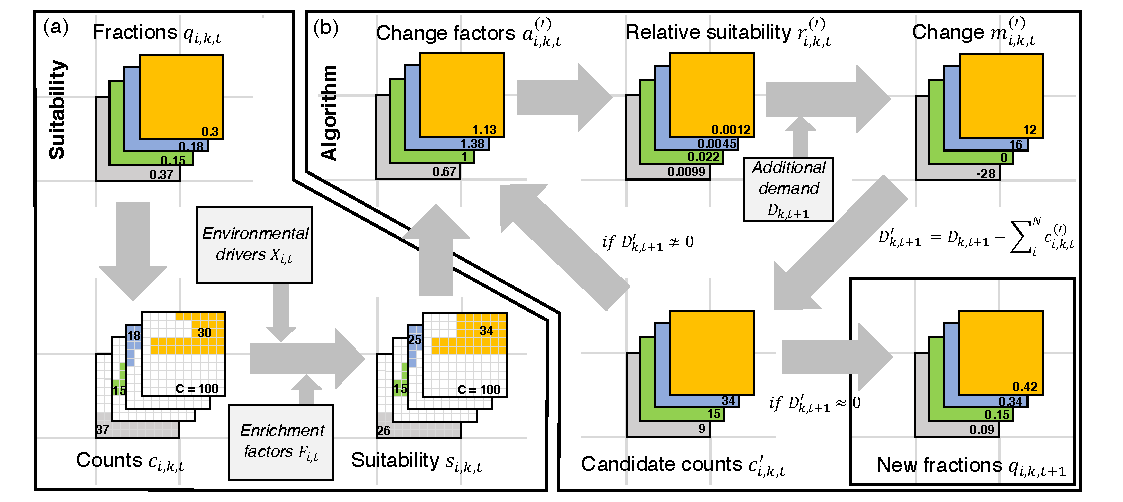
\includegraphics[width=1\linewidth]{chapters/figures/chapter3/fig1.pdf} 
    \caption{Conceptual diagram of land use modelling approach. (a) Land use suitability model. Observed fractions of land use are first converted to integer counts through multinomial draws and their relationship with environmental drivers and neighbourhood covariates (derived from previous time steps land-use distribution) is assessed. (b) Allocation algorithm. First, it is estimated by how much each cell has to change to achieve the modelled ideal distribution of land uses. Change factors are then converted to relative suitabilities that serve to distribute land use supply required to satisfy the additional demand in the landscape. Multinomial draws ensure that each cells land use class probabilities sum to 1. The resulting difference of the current supply and the total additional demand is recalculated to support allocation in the next iteration. The cycle repeats until the difference between the current supply and total additional demand is very close to zero, meaning that all additional demand has been allocated. At this point, the integer counts representing the land use fractions on each cell are converted back to fractional representation. The new fractions are used to calculate neighbourhood covariates in the next time step.}
    \label{ch3:fig1}
\end{figure*}

\subsubsection{Rule 1: Future land use supply meets additional demand}

Projections of land use demands may be provided through external models, such as Computational General Equilibrium (CGE) models \citep[i.e.~GTAP,][]{aguiar_overview_2016}), or through the analysis and extrapolation of historic patterns \citep{moulds_open_2015}. The model allocates additional demand by adding cell-level supply of that time step \(d_{i,k,t+1}\) in cell \(i\), land use \(k\) and time step \(t+1\) to the fractions of the current time step \(q_{i,k,t}\) (\Cref{ch3:fig1}b). The first model objective can be formulated:

\begin{equation}
 \begin{aligned}
\sum_{i=1}^N q_{i,k,t+1} = \sum_{i=1}^N (q_{i,k,t} + d_{i,k,t+1})\\
\end{aligned}
\end{equation}

\begin{equation}
 \begin{aligned}
\sum_{i=1}^N d_{i,k,t+1} = D_{k,t+1}
\end{aligned}
\end{equation}

\(D_{k,t+1}\) is the additional landscape-wide supply and is at
equilibrium with additional demand after the algorithm converges.

\subsubsection{Rule 2: Cell-level fractions must sum to1}

The second model condition requires that supply of all land-use types in
a cell \(d_{i,k,t+1}\) is allocated across cells so it adds up to one (\Cref{ch3:fig1}b):
\begin{equation}
\begin{aligned}
\sum_{k=1}^K q_{i,k,t+1} = 1
\end{aligned}
\end{equation}

\subsubsection{Rule 3: Allocations are determined by land use
suitability}

The third model condition requires cell-level supply \(d_{i,k,t+1}\) to
be distributed in such a way that the allocated amounts in each cell
scale with a predicted probability surface \(s\), by modelling
\(q_{i,k,t=0} \approx s_{i,k}=f^k(\mathbf{X_i})\), where \(X_i\) is a
set of demographic and bio-physical drivers related to land use. \(f^k\)
is a multinomial, multi-response model (\Cref{ch3:fig1}a). The
parameter estimation of this model is based on the first time step and
predicted to the conditions of subsequent time steps. Accordingly, while
the model assumes stationarity of the modelled statistical
relationships, it implements temporal dynamics based on changing demand
and changing environmental conditions. Changing environmental conditions
are represented as changes to independent model variables.

The land use status in a cell's neighbourhood has been shown to play an
important role in determining a cell's land use
\citep{dendoncker_spatial_2007, mustafa_modelling_2018, van_vliet_measuring_2013, verburg_method_2004}.
Our suitability model applies neighbourhood interactions by calculating
autocovariates \citep{verburg_method_2004} and including these in the
multinomial regression of the land use suitability model. Following
\citet{verburg_method_2004}, our autocovariates measure the amount of
clustering of land uses in the cell neighbourhood when compared to the
entire landscape. We calculate autocovariates as enrichment factors
\(F_{d,i,k,t}=\frac{\sum_{i \in d} (q_{i,k,t})/N_d}{\sum_{i=1}^N (q_{i,k,t})/N}\).
The numerator is the average fraction of land use \(k\) in the
neighbourhood \(d\) of each central cell \(i\) and the denominator is
the average fraction of land use \(k\) in the entire landscape \(N\).
Here, we only included neighbourhood characteristics in the \(3x3\)
neighbourhood around each central cell, but other neighbourhoods are
possible \citep{verburg_method_2004}. When predicting suitability at
each time step, the autocovariates are recalculated based on the
assigned fractions from the previous timestep.

Our response variable is a fractional land use value, not discrete
classes normally required in multinomial regression. Therefore, we
assume that underlying the land use fractions for each cell is a vector
of counts \(c_{i,k,t}\) that sums to a total number of counts \(C\) in
each cell (e.g.~\(C=1e6\)). We derive these counts through
\(c_{i,k,t} \approx q_{i,k,t} * C\). In integer representation, the data
are approximately proportional to the original fractions. When fitting
the suitability model, parameter uncertainty depends on the assumption
of \(C\). \(C\) should be chosen to represent the degree of numerical
precision in the observed fractions. For example, if there are only 2
decimal places, setting \(C = 100\) results in counts that represent all
of the information contained in the original fractions. Accordingly, the
multinomial logit model takes the form

\begin{equation}
\begin{aligned}
s_{i,k,t}= P(Y_{i} = k) = \frac{e^{\beta_{k} * X_{i,t} + \gamma_{d,k}*F_{d,i,k,t}}}{\sum_{k=1}^k e^{\beta_{k} * X_{i,t}+ \gamma_{d,k}*F_{d,i,k,t}}}
\end{aligned}
\end{equation}

where \(k\) is the reference land use class, \(\beta_{k}\) the estimated
parameters in each class for covariates \(X_{i,t}\) and \(\gamma_{d,k}\)
the estimated parameters for autocovariates \(F_{d,i,k,t}\). We
estimated parameters using R's `nnet' package
\citep{venables_modern_2002}. Predicted fractions satisfy
\(\sum_{k=1}^K s_{i,k,t} = 1\).

All software development and model validation was conducted in \texttt{R} (version 4.0.1) \citep{r_development_core_team_r_2008}.

\subsection{Data}

We developed and tested our model using land use and environmental data
from the Amazon basin. We downloaded 7 time steps (1992, 1997, 2003,
2008, 2013, 2015 and 2018) of the global land cover map provided through
the European Space Agency's Climate Change Initiative Land Cover
(CCI-LC) project \citep{esa_land_2019}. These data are available at a
grid resolution of 300m. We combined the recorded 31 land cover classes
to 9 new classes of land use we deemed crucial to identify processes
leading to agricultural expansion and declines in habitat (\Cref{ch3:tab2}). We aggregated the resolution
10km\textsuperscript{2} squares, calculating fractions of land use from
the cell counts of each land use class on the original map present in
each new cell. Fractional land use in \(K\) classes is mapped over \(N\)
raster cells, with fractions \(q_{i,k,t}\) in cell \(i\) in each land
use class \(k\) always satisfying \(0\leqslant q_{i,k,t}\leqslant 1\)
and \(\sum_{k=1}^K q_{i,k,t} = 1\).

\begin{table}[htb]
\setlength\tabcolsep{4pt} % default: 6pt
\caption{Mapping of original land use classes to new classes applied in this study}  
\label{ch3:tab2}
\begin{tabularx}{1\textwidth}{@{}llllY@{}}
\toprule 
  & New class & Abbr. & CCI-LC class & Description \\
\toprule 
1 & Cropland & Cro & 10, 11, 12, 20, 30 & Rainfed and irrigated cropland, mosaic cropland with \textgreater 50\% cropland and natural vegetation (tree, shrub, grass) \\ 
2 & Cropland mosaic & CrM & 40 & Mosaic cropland with \textless 50\% cropland and natural vegetation (tree, shrub, grass) \\ 
3 & Forest & For & 50, 60-62, 
                70, 80, 90, 100, 160, 170 & Forest, closed to open, with \textgreater 15\% canopy cover, Mosaic tree/shrub (\textgreater 50\%) / herbacious cover, Flooded tree cover \\ 
4 & Grassland & Gra & 110, 130 & Grassland and mosaic herbacious cover (\textgreater 50\%) / tree/shrub \\ 
5 & Shrubland & Shr & 180 & Closed to open and open shrubland \\ 
6 & Wetland & Wet & 190 & Flooded shrub or herbacious cover \\ 
7 & Urban & Urb & 120 & Settlement, Urban land uses \\ 
8 & Other & Oth & 140, 150, 151-153, 200-202, 220 & Lichen/mosses, sparse trees/shrubs/herbaceous vegetation, bare areas, snow/ice \\ 
9 & Inland water & Wat & 210 & Natural and artificial inland water bodies \\
\bottomrule
\end{tabularx}
\end{table}

We downloaded a set of spatially explicit climate, topographic soil and
human covariates (\Cref{ch3:tab3} for a full list of
covariates), derived neighbourhood covariates from observed land use in
the first time step and estimated observed demand change by calculating
the landscape-wide mean fraction for each land use class in each
observed time step. All explanatory covariates were standardized to have
mean 0 and standard deviation 1. We removed covariates from correlated
pairs (Spearman's rank correlation coefficient \(> 0.7\)), always
retaining the covariate with the smaller average correlation with all
other covariates in order to maximise the amount of independent
information in the final data set used for fitting.

\begin{table}[htb]
\setlength\tabcolsep{4pt} % default: 6pt
\caption{List of covariates that were included in land use suitability model}  
\label{ch3:tab3}
\footnotesize 
\begin{tabularx}{0.8\textwidth}{@{} llll@{}}
\toprule 
Type & Covariate name & Source \\
\toprule
climate & Annual mean temperature & \cite{fick_worldclim_2017} \\
& Mean diurnal range & \\
& Isothermality & \\
& Temperature seasonality & \\
& Max. temperature of warmest month & \\
& Min. temperature of coldest month & \\
& Temperature annual range & \\
& Mean temperature of wettest quarter & \\
& Mean temperature of driest quarter & \\
& Mean temperature of warmest quarter & \\
& Mean temperature of coldest quarter & \\
& Annual precipitation & \\
& Precipitation of wettest week & \\
& Precipitation of driest week & \\
& Precipitation of driest month & \\
& Precipitation of wettest quarter & \\
& Precipitation of driest quarter & \\
& Precipitation of warmest quarter & \\
& Precipitation of coldest quarter & \\
topographic & Roughness & \cite{hijmans_very_2005} \\
& Slope & \\
& Elevation & \\
& Distance to coast & \cite{wessel_global_1996}\\
& Distance to lake & \\
soil & Nitrogen Content & \cite{global_soil_data_task_group_global_2000}\\
& Available Water Content & \\
& Carbon Density & \\
& Bulk Density & \\
human & Distance to built-up areas & \cite{fao_built-up_1997}\\
& Distance to highways & CIESIN (\citeyear{center_for_international_earth_science_information_network_-_ciesin_-_columbia_global_2013})\\
& Distance to private roads & \\
& Distance to trails & \\
& Protected areas & \cite{iucn_world_2014} \\
\bottomrule
\end{tabularx}
\end{table}

\subsection{Model constraints}

Analysing time series data, we determined that only very small
percentages of cells change from being devoid of a particular land use
to containing that land use within one time step (\Cref{ch3:tab4}). To control unrealistic dispersal of land uses into
areas where they have not previously existed, we added a constraint that
land use increases are more likely to be applied to cells where the land
use is already present. The constraint parameter was the percentage of
cells in which a non-existent land use was newly established between
time steps. For example, setting the constraint to 100\% would allow
increases of a land use in all cells that did not contain that land use
in the previous time step.

We parametrized the constraint by determining on how many cells
(expressed as a percentage) we could observe the new establishment of a
land use from one time step to the next (\Cref{ch3:tab4}). To
account for annual variation, we calculated the mean of these
percentages for each land use throughout the entire observed time
series. For example, throughout the simulation, we allowed \emph{Cro}
increases in 1.35\% of the cells in which \emph{Cro} was not present in
the preceding time step (\Cref{ch3:tab4}). We selected those
cells for new establishment of a land use that had the highest predicted
suitability for that land use (see \Cref{apx:ch3} for more information on
this constraint).

We masked category I and II protected areas established up until 1992
from land use changes as has been shown previously (see
\Cref{ch3:fig2} for a map of protected areas)
\citep{verburg_modeling_2002, iucn_world_2014, kapitza_assessing_2021}.
To reflect the high initial investment of urban infrastructure, we did
not allow reductions in urban land \citep{verburg_combining_2009}.

\begin{table}[htb]
\captionsetup{width=.5\textwidth}
\caption{Share of cells ($\%$) containing a land use that were completely devoid of that land use in the preceding time step. Values derived from observed time series.}  
\label{ch3:tab4}
\footnotesize
\centering
\begin{tabularx}{.5\textwidth}{@{}lXXXXXXX@{}}
\toprule 
Land use & 1996 & 2001 & 2006 & 2011 & 2016 & 2018 & mean \\ 
\toprule 
Cro & $1.75$ & $1.66$ & $4.49$ & $0.08$ & $0.06$ & $0.07$ & $1.35$ \\ 
CrM & $2.39$ & $2.37$ & $7.24$ & $0.05$ & $0.03$ & $0.05$ & $2.02$ \\ 
For & $0$ & $0$ & $0$ & $0$ & $0$ & $0$ & $0$ \\ 
Gra & $0.40$ & $0.62$ & $0.94$ & $0.15$ & $0.04$ & $0.04$ & $0.37$ \\ 
Shr & $0.62$ & $0.90$ & $1.44$ & $0.15$ & $0.07$ & $0.06$ & $0.54$ \\ 
Wet & $0.62$ & $0.68$ & $2.60$ & $0.26$ & $0.13$ & $0.11$ & $0.73$ \\ 
Urb & $0.36$ & $0.61$ & $1.12$ & $0.16$ & $0.28$ & $0.02$ & $0.43$ \\ 
Oth & $0.02$ & $0.06$ & $0.12$ & $0.05$ & $0.02$ & $0.01$ & $0.05$ \\ 
Wat & $0.81$ & $0.35$ & $1.19$ & $0.02$ & $0.01$ & $0.01$ & $0.40$ \\ 
\bottomrule 
\end{tabularx} 
\end{table}

\subsection{Validating the intensity and direction of predicted
changes}

First, we examined the accuracy of the multinomial suitability model and
how it is affected by spatial resolution and the included covariates. To
account for spatial autocorrelation in the environmental covariates and
land use time series, we conducted spatial-blocks cross-validation
\citep{valavi_blockcv:_2019} by separating the landscape into 9
equal-sized spatial blocks. We fitted models using data from 8 of the 9
blocks and predicted the model to the withheld block, until predictions
were made for the entire study area. We cross-validated suitability
models at 1km and 10km, including 1) only environmental covariates, 2)
only neighbourhood covariates and 3) both covariate types combined. For
each of the three models we measured predictive performance by
estimating cell-level suitability Root Mean Squared Error
(RMSE\textsubscript{suit}) between the predicted suitability surfaces
\(s_{m,i,k,t}\) and the observed fractions \(o_{i,k,t}\), following

\begin{equation}
\begin{aligned}
RMSE_{suit,m,i,t} = \sqrt{\frac{1}{K} \sum_{k=1}^K(o_{i,k,t}-s_{m,i,k,t})^2}
\end{aligned}
\end{equation}


for each suitability model \(m\).

Second, to validate the intensity of changes predicted by the allocation
algorithm, we assessed the accuracy of predictions of cell-level
fractions under competing models predicted throughout the observed time
series. 1) Under the null model, we assumed no change of land use
through time. The null model served as reference to measure the
improvements provided by each additional model component. 2) Under the
naive model we only allocated additional demands, but scaled cell-level
allocations with the average supply observed across the entire
landscape. This model assumes that suitability is not informative about
where a change will happen and that allocations are equally likely to be
anywhere in the landscape. 3) Under the semi-naive model, cell-level
allocations were additionally scaled with the predicted suitability
surfaces \(s_{i,k,t}\) (as illustrated in \Cref{ch3:fig1}). 4)
Under the full model, allocations were scaled with suitability surfaces
\(s_{i,k,t}\) and all constraints (constraining most increases to cells
where land use type already exists and masking protected areas from
changes) were applied.

We calculated RMSE\textsubscript{alloc} under each allocation model
\(w\) to estimate how well the different model components simulated each
cell-level vector of land use fractions \(q_{m,i,k,t}\) compared to the
respective observed vectors \(o_{i,k,t}\), following

\begin{equation}
\begin{aligned}
RMSE_{alloc, w,i,t} = \sqrt{\frac{1}{K} \sum_{k=1}^K(o_{i,k,t}-q_{w,i,k,t})^2}
\end{aligned}
\end{equation}

Due to the squared term, RMSE cannot inform on whether the models
correctly identified the direction of change. Therefore, we estimated
and validated the direction of cell-level changes (decreases, no change,
increases) separately. We mapped these transitions for each class
between the time steps of the observed time series and the time steps of
the time series simulated under each model. We calculated \emph{overall
difference} of each pair of corresponding maps to obtain an
interpretable measure of similarity of predicted and observed direction
of changes \citep{pontius_death_2011, pontius_quantity_2014}. Achieving
high accuracy in these first two model goals would suggest that
simulated patterns of land use change closely resemble observed
patterns.

\subsection{Case study: agricultural expansion in the Amazon
Basin}

The Amazon catchment is largest river basin in the world and occupies
over one third of the South American land mass (\Cref{ch3:fig2}a). As the world's most diverse tropical forest area,
the basin hosts at least 10\% of the world's known species
\citep{da_silva_fate_2005}.

\begin{figure}[htb]
\centering
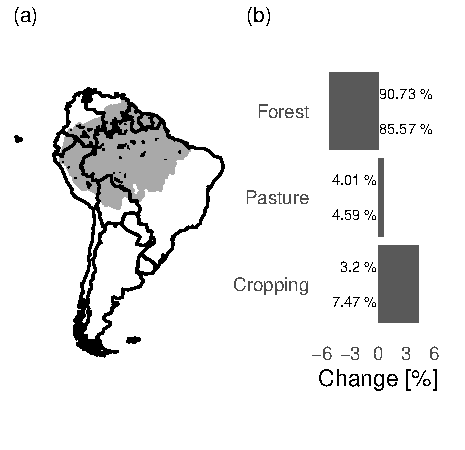
\includegraphics[width=3.11in]{chapters/figures/chapter3/fig2.pdf} 
\caption{Overview of the study area. (a) Location of the amazon catchment in South America (grey-shaded area), including IUCN protected areas (categories I and II) which were used to constrain land use changes (black shaded areas). (b) Changes in selected land uses, derived from observed land use maps. Pasture includes Gra and Shr, Cropping includes Cro and CrM and forest includes For. Beside the bars are percentage cover in 1992 (top) and percentage cover in 2018 (bottom). Land use classes are specified in \Cref{ch3:tab3}.}
\label{ch3:fig2}
\end{figure}

The Amazon biome is threatened by a multitude of interacting factors.
Ecosystem services, such as water supply, carbon storage and provision
of species habitat are directly threatened by the effects of climate
change and the increasing pressure on land, with projected severe
reductions in water yields, carbon content and species habitat, which is
particularly affected by changes in natural vegetation cover
\citep{prussmann_vulnerability_2016}. The primary uses for cleared
forest land are pasture for cattle farming and industrial soy cropping
\citep{nepstad_slowing_2014, fao_aquastat_2015}. Between 1992 and 2018,
the biome has seen significant increases in land required for cropping
and pasture, as well as significant decreases in forest cover (\ref{ch3:fig2}b).

Using a broad reclassification of the predicted and observed land use
classes into cropland, pasture and habitat, we were able to specifically
validate our model's ability to predict agricultural expansion and
habitat declines as aggregated threats to ecosystems and biodiversity.
First, we determined areas of agricultural (pasture or cropland)
expansion with simultaneous declines in classes containing natural
habitats (\emph{For}, \emph{Wet} and \emph{Oth}). We categorized the
observed and predicted maps into 1) areas with no cropland increase, 2)
areas where cropland increase led to mostly forest declines (net
replacement of forest), and 3) areas where cropland increase led to
mostly declines in other natural habitat classes (net replacement of
other habitat). Similarly, we categorized the landscape into 1) areas
with no pasture increase, 2) areas where pasture increase led to mostly
forest declines, and 3) areas where pasture increase led to mostly
declines in other natural habitat classes. From the resulting
reclassified time series we assessed the difference between the
respective observed and predicted maps by overlaying them and
identifying where no agricultural increase was observed and predicted
(persistence predicted as persistence), where agricultural increase was
correctly predicted and led to decreases in the correct habitat class,
where agricultural increase was correctly predicted but resulted in
decreases in the incorrect habitat class, where no agricultural increase
was observed, but agricultural increase was predicted, and where
agricultural increase was observed, but not predicted
\citep{pontius_comparison_2011}.

\section{Results}

\subsection{Predicting land use change intensity}

Results of the cross-validation of the suitability model component show
that including neighbourhood covariates resulted in substantial
predictive performance improvements across spatial blocks at both
resolutions (\Cref{ch3:fig3}c); models using neighbourhood
covariates alone were approximately as good as the model using the full
covariate set. Including only environmental variables resulted in less
accurate predictions at both resolutions, with predictions under the
fine resolution comparatively worse than under the coarse resolution.

\begin{figure}[htb]
\centering
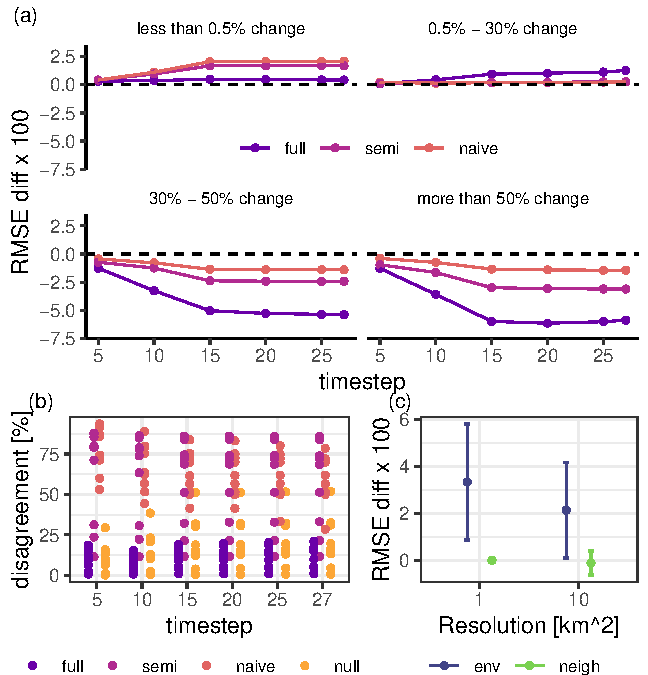
\includegraphics[width=4.33in]{chapters/figures/chapter3/fig3.pdf} 
\caption{Validation of predicted land use change intensity and direction of change and cross-validation of suitability model. a) The difference between RMSE for each model (naive, semi-naive, full) and RMSE of the null model. The null model assumes that land use is static through time, the naive model assumes completely random allocations, the semi-naive model assumes that allocations are scaled with land use suitability and the full model assumes that allocations are both scaled with land use suitability and subject to model constraints (no changes in areas under high protection status and no land use increases in areas completely devoid of that land use). All RMSE were calculated at cell-level, using the predicted and observed vectors of land use fractions in each cell. Plotted are means across cells. Positive values indicate better fits under the null model, negative values indicate better fit under more highly parametrised models. Data on validation outcomes are grouped by the magnitude of the largest observed proportional change in any land use within a cell. In general, the larger the observed change in land use, the better the parameterized models did compared with the null model. b) The proportional disagreement between predictions of the cell-level direction of change (no change, decrease, increase) for each land use and the observed direction of change at each time step. Smaller values indicate lower overall difference and higher similarity between corresponding maps. c) Difference between cross-validated RMSE estimated for suitability models containing only environmental covariates and only neighbourhood covariates and models containing both covariate types combined. Positive values indicate a poorer fit than the model containing both covariate types.}
\label{ch3:fig3}
\end{figure}

Under all tested models (naive, semi-naive, full), the accuracy of
cell-level allocations improved with the intensity of observed changes
(\Cref{ch3:fig3}a). This implies that our model makes good
predictions under scenarios with high expected overall changes.

Where observed changes were large (\Cref{ch3:fig3}a, bottom
two panels), including land use suitability and constraints (full model)
resulted in substantial increases of predictive performance. In these
areas, the null model's assumption of no spatial variation in
reallocation of land use introduced very high bias, which our
constraints were able to reduce.

When observed changes were small (\Cref{ch3:fig3}a, top two
panels), the null model made near perfect predictions. Given how close
the null model already was to the truth, improvements by allocating
demand (naive model) and accounting for land use suitability (semi-naive
model) were difficult to achieve; in the smallest change category (\Cref{ch3:fig3}a, top left panel), the naive and semi-naive
predictions were in fact slightly worse than the null. In these areas
the largest observed changes were below 0.5\%, making the assumption of
no change under the null model highly plausible. Under the full model,
the applied constraint limited the areas that could be flagged for
increases. Accordingly, where observed changes were small, this model
made better predictions than the semi-naive and naive models, in which
this constraint was not applied.

\subsection{Predicting the direction of land use
changes}

The worst predictions of cell-level direction of change were made by the
naive and semi-naive models and the best predictions under the full
model \Cref{ch3:fig3}b), with overall difference consistently
less than 25\%. Predictions became more accurate the more model
components were applied. Under the full model we achieved the highest
prediction accuracy. Overall, the semi-naive model performed slightly
better than the naive model, demonstrating the utility of scaling
allocations with land use suitability surfaces.

\subsection{Predicting agricultural expansion and habitat
declines}

Our model achieved high accuracy when predicting agricultural (cropland
and pasture) expansion on forest and other land use types containing
natural habitats (\Cref{ch3:fig4}). In more than 80\% of cells
our model predicted correctly whether agricultural land (cropland or
pasture) increased, or persisted at current levels or decreased, and
which habitat type decreased due to increases in agricultural classes
(\Cref{ch3:fig4}b, d).

\begin{figure}[htb]
\centering 
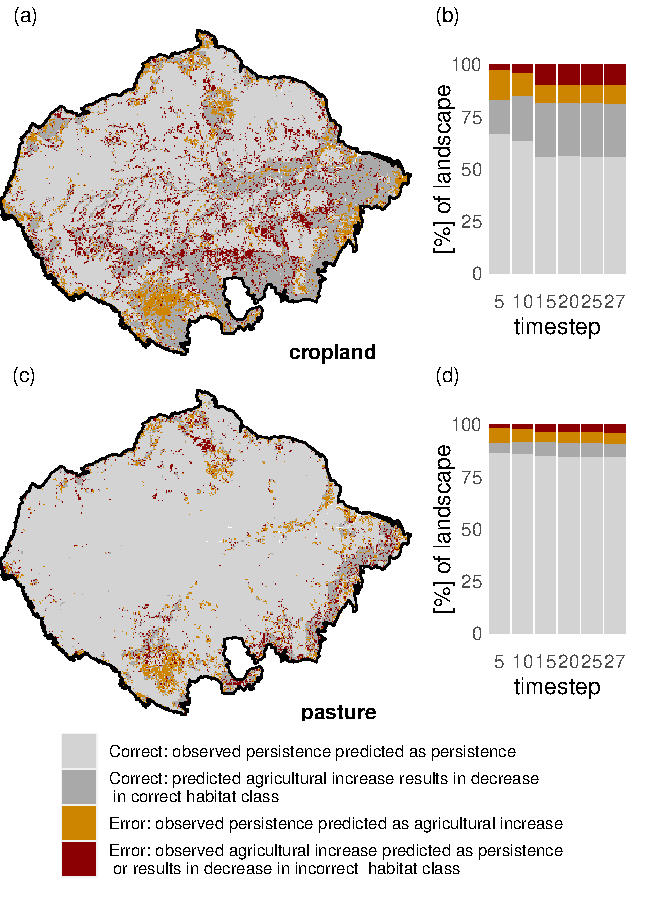
\includegraphics[width=4.33in]{chapters/figures/chapter3/fig4.pdf}
\caption{Validation of modelling agricultural expansion in cropland and pasture on forest and other natural habitat types in the Amazon basin. (a, b) Spatial configuration of correct and erroneous predictions of cropland in the last time step of the validation time series (2018) (a) and the relative size of the landscape where predictions matched observations (correct) and where predictions deviated from observations (error) in cropland (b). (c, d) Spatial configuration of correct and erroneous predictions of pasture in the last time step of the validation time series (2018) (c) and the relative size of the landscape where predictions matched observations (correct) and where predictions deviated from observations (error) in pasture (d).}
\label{ch3:fig4}
\end{figure}

The percentage of the landscape in which we correctly predicted cropland
increase at the expense of the correct habitat class increased through
the time series, suggesting that our model was good at identifying not
only where cropland did not change or decreased (persistence), but also
where it increased and on which habitat type that increase took place
(\Cref{ch3:fig4}b). Our model made some incorrect predictions of
cropland increase in areas where no increase was observed in the
southern tip and the central north of the study area, although these
areas were very small compared to surrounding areas in which increases
were correctly predicted and occurred on the appropriate habitat classes
(\Cref{ch3:fig4}a). Perhaps the most severe type of error in
terms of ecological considerations was the prediction of no cropland
increase (persistence) in areas where increase was observed. However,
these areas were small (increasing from 2.3\% of the landscape at the
beginning to 9.6\% at the end of the time series).

Pasture expansion (\Cref{ch3:fig4}c, d) was much smaller than
cropland expansion overall, with much larger areas of the basin
correctly predicted as not increasing in pasture land (persistence)
through time (\Cref{ch3:fig4}d). Some small areas in the
southern tip, the central north and along the western boundary of the
basin were correctly predicted to increase in pasture land, with
decreases in the appropriate natural habitat class. Pasture expansion
was underpredicted in very small areas in the south, north and along the
eastern boundary of the basin (\Cref{ch3:fig4}c).

\section{Discussion and conclusions}

We have presented a new land use model to predict land use fractions,
thus retaining information at sub-pixel level. The model is able to
accurately allocate fractions of land use through time, especially under
scenarios of more extreme land use change. We explicitly accounted for
competition between land use types and land use suitability in response
to environmental drivers by means of a multinomial logistic model and
could show that this aspect brings substantial improvements to
predictions, when compared to the assumption that land use does not
change at all (null model).

Our model made accurate predictions in areas in which only small land
use changes were observable, but also in areas where land use changes
were observed to be high. This suggests that our model provides a
suitable method to produce future land use maps under contrasting
scenario settings. In scenarios where demand changes are expected to be
high, our model allocates supply to match aggregated demand, changing
the total area allocated to different land uses and also allowing land
uses to be established in new areas. In scenarios with small expected
demand changes, land use changes, including the establishment of land
uses in new areas, remain small.

We assumed that the initial land use distribution we used to calibrate
our model resulted from long time periods of optimizing behaviour and we
have not yet implemented a parameter allowing to specify land use
elasticity (the propensity of land uses to shift across the landscape
without net changes to their total areas at the study area level), as is
implemented, for example, in Dyna-CLUE \citep{verburg_combining_2009}.
For this reason, in our model land use cannot change to match predicted
land use suitability alone. For example, if the modelled cropland
suitability in an area is 0.8, but the observed cropland fraction is
0.2, our model would only allow a local increase in cropland if the
aggregated demand for cropland at the study area level increased. While
the discrepancy between an area's potential for a certain land use
measured by the predicted suitability and the realized fraction of that
land use implicitly captures processes that cannot be captured by the
suitability model, in this first version of our model this only occurs
when triggered by changes in external demand for that land use.

Similar to CLUE, our constraint on turn-over allowed us to account for
conversion effort. Here, data from the observed validation time series
allowed us to extract a raw estimate of the constraint parameter to tune
our model. We estimated the parameter using long-term observed means. We
assume this to be similarly informative as informal expert knowledge,
which has been suggested as a primary means to parametrize land use
conversion effort in previous land use models
\citep{van_asselen_land_2013, overmars_comparison_2007}.

We could show that our model is very easily adaptable to specific
ecological study contexts. When validating our model's performance in
the context of agricultural expansion on natural habitat, we mapped the
model's ability to reproduce where agricultural expansion occurs in both
pasture and cropland and which natural habitat classes decreased in
their place. Consistently more than 80\% of the landscape where
correctly classified as no change or a decrease (persistence) or
increase of agricultural land with decreases in the correct habitat
types. Crucially, underprediction of agricultural expansion with
possible negative implications for conservation management remained very
small throughout. This demonstrates that our model is a useful tool to
predict the spatial configuration of land use change impacts that are
driven by agricultural expansion into different habitat types.

Validating the suitability model component of our model approach, we
found that neighbourhood covariates explained much of the suitability
patterns across the landscape. This is a common effect of including
flexible spatial correlation terms in models with other
spatially-varying covariates (spatial confounding)
\citep{hodges_adding_2010}. The models describe the spatial pattern with
the spatial correlation term, but this effect does not imply causation
and other drivers included in the model may still drive changes in the
response, particularly over long time periods. Here, similar to what was
shown by \citet{dendoncker_spatial_2007}, including neighbourhood
covariates lead to the most highly fitted models. Allowing spatial
autocorrelation to drive patterns seems a sensible choice for
predictions in this case study because the model only predicts three
decades. However, for longer time spans, spatial autocorrelation
probably becomes less important and continental-scale environmental
driving factors acting homogeneously across the whole landscape may
dominate patterns in reality. When making such longer-term predictions,
this could be captured by fitting the suitability model with several
time steps of data, thus ensuring that land use suitability is less
reliant on the present land use state, but more weight is given to
long-term and large-scale environmental processes.

The results of our validation also strongly indicate that in case of our
model, adding constraints (decision rules) in terms of where and how
land use changes are allowed to occur, are responsible for the majority
of increases in predictive performance. While we provide initial steps
in parametrising these constraints, more specific knowledge of bottom-up
processes that drive land use stasis and change across the landscape
could further consolidate the accuracy of our model. For example, this
could be achieved by including data on the expected behaviour of
economic agents who seek to maximise returns on their productive land.
One example includes the Land Use Trade-offs (LUTO) model
\citep{bryan_supply_2014, connor_modelling_2015}, which includes
pixel-wise optimisation of cost and return of alternative land uses.
However, such models are difficult to parametrise in data-scarce regions
and require significant computational power. Bottom-up processes, such
as price feedbacks, also tend to act at very fine spatial resolutions,
but have little effect when seen at a continental scale, where scenario
uncertainty and global processes dominate predictions
\citep{connor_modelling_2015}. Depending on scale, including very
fine-scale dynamics of agent behaviour may simply not pay off, or it
might be more appropriate to merely downscale them to the study area
extent \citep{van_asselen_land_2013, connor_modelling_2015}.

In order to allow scaling our model to global applications, we only used
drivers that were available at global scales. However, improvements to
the land use suitability model can be achieved by including more
proximate drivers of land use change, such as market accessibility
\citep{meiyappan_spatial_2014, verburg_global_2011}, by fitting the land
use suitability model for individual subsets of the study area to
improve local fit, or by creating more land use classes for which
particular biophysical constraints are known. Including
location-dependent drivers and models and raising the resolution may
substantially improve the accuracy of land use suitability maps,
increasing the contribution of this model component to overall
prediction accuracy.

Developments of our model and expanding application could include the
estimation of use intensity of different land use types, which has been
shown to be an important driver of biodiversity change
\citep{newbold_global_2015, newbold_has_2016}. Such developments could
enhance efforts to tailor macroeconomic and land use modelling to assess
the fate of future biodiversity \citep{kapitza_assessing_2021}.

\section{Acknowledgements}

We are grateful for contributions made throughout the research phase by
J. Elith and D. Zurell and helpful comments by Robert G. Pontius Jr on a
preprint of this manuscript. Funding: this work received funding under
the Australian Research Council Discovery grant DP170104795. NG was
supported by an ARC DECRA fellowship (DE180100635). SK was supported by
the Melbourne International Research Scholarship (MIRS).

\chapter{Toward streamlined and transparent economic-ecological predictions of land-use change impacts on biodiversity}
\label{ch4}
\newpage

\section{Abstract}

Climate and land-use change are two of the most impactful drivers of global biodiversity change, but integrated assessments of the impacts of these drivers on biodiversity are rare and tend to be highly complex and not repeatable by analysts other than those who developed them. We have developed a dramatically simplified, more transparent, and transportable integrated biodiversity assessment framework and modelling apparatus that can be modified and adapted to a broad array of integrated biodiversity assessment contexts. Our framework is applicable to a range of fundamental questions about the combined impacts of economy, climate change and land-use change on biodiversity. Here, we address how closely our framework approximates more complex, more highly parameterized, and less transparent and repeatable integrated assessment modelling (IAM) frameworks in terms of predictions about biodiversity change under future socio economic scenarios. We utilize our framework to predict future global biodiversity intactness under two so-called `Shared Socio-economic Pathways' and compare our predictions to those derived from the `Message 8.5' IAM. We find that predicted changes of biodiversity intactness are smaller when using our simplified framework compared with predictions derived from the Message 8.5 IAM.  Differences in predicted biodiversity intactness are mainly due to differences in the predicted availability of ‘natural’ habitats, which are predicted to be more extensive under our framework. Our chosen model to predict conversions between habitat types was based on the predicted average suitability of land for these habitat types and approximates recent historic patterns, suggesting that this approach is plausible. We showcase the first global implementation of a simple modelling framework that is more transparent, interpretable, and reproducible than most other IAM.

\section{Introduction}

\subsection{Multiple threats to future biodiversity}

Biodiversity change is driven by the direct exploitation of organisms, climate change, land/sea-use change, pollution, and the invasion of alien species \citep{ipbes_summary_2019}.

Climate change and land-use change are of particular significance for biodiversity and are likely to cause significant distributional changes, reduction in biodiversity, and further extinctions of species \citep{ipbes_summary_2019, struebig_targeted_2015, newbold2019climate, kapitza_assessing_2021, foley_global_2005}. Climate change affects the distributional ranges of species directly by impacting on their biophysical niches and indirectly by altering global land-use patterns \citep{kapitza_assessing_2021}. 

Despite the importance of these drivers, land-use and climate change impacts on biodiversity are usually considered in isolation and only few examples exist in which synergistic impacts are examined, probably leading to the underestimation human impacts on biodiversity \citep{de_chazal_land-use_2009}. Interactions between climate and land-use on biodiversity also depend on the regional context and global economic processes that may play out across continents. For example, direct climate change impacts on biodiversity have been observed to overshadow indirect impacts \citep[where climate change affects species distributions via impacts on land use, \Cref{ch1},][]{kapitza_assessing_2021}. However, the opposite may occur if global telecoupling of consumption and production patterns displace impacts on biodiversity to other locations. Such indirect impacts of climate change on biodiversity cannot be understood, assessed or predicted without explicitly considering economic trade. Regions where land becomes less productive under climate change may increase imports of agricultural commodities and export impacts of increasing agricultural land demands to other regions \citep{kapitza_assessing_2021, chaudhary_land_2016}. To alleviate prediction uncertainty caused by these complex macro-economic linkages, it is critical to deepen our knowledge of when and where land-use changes and associated biodiversity impacts may occur in response to macro-economic dynamics; not only under climate change, but also under other socio-economic changes.

\subsection{Integrated biodiversity assessments}
It has been broadly acknowledged that assessments of future biodiversity require integrated, flexible models that deploy methods from various disciplines \citep{ipbes_summary_2019}, but frameworks combining such methods specifically with biodiversity in mind are still lacking \citep{titeux_global_2017}. Existing institutional-scale, integrated assessment models (IAMs) have been widely adopted to inform climate change mitigation policy, although in that capacity they have tended to focus on the assessment of socio-economic and other non-human environmental factors, such as population growth, greenhouse-gas emissions, radiative forcing, land-use change, and climate mitigation potential \citep{riahi_shared_2017}. Despite the high level of institutional support and technical finesse, IAMs were not designed to deliver fine-tuned predictions of biodiversity impacts \citep{harfoot_integrated_2014}.

However, this situation is slowly changing, as research concerned with predicting future environmental conditions to inform policy-making is becoming increasingly interdisciplinary. Bespoke frameworks that cross disciplinary boundaries have been developed for integrated assessments of biodiversity change \citep{newbold2019climate, kapitza_assessing_2021, leclere_bending_2020} and IAMs have recently been deployed to predict regional biodiversity outcomes to inform sustainable development policy \citep{veerkamp_future_2020}, confirming that biodiversity is increasingly being acknowledged as a crucial aspect of sustainable policy-making.

\subsection{Shared future narratives}
Efforts to harmonize future predictions made by IAMs have resulted in the formulation of narratives about future socio-economic conditions that clearly delineate the assumptions for alternative future scenarios \citep{oneill_new_2014, oneill_roads_2017}. These `Shared Socio-economic Pathways' (SSP) \citep{oneill_new_2014} provide the narrative basis for models to determine reduction targets for greenhouse-gas-emissions and to inform global land-use policy, but also for the macro-economic analyses of policy instruments, such as the transition to low-carbon energy \citep{riahi_shared_2017}. 

The main advantage of these narratives are the shared sets of assumptions about alternative, plausible futures that clearly outline the socio-economic environment within which sustainable policy-making takes place. For example, the \textit{scenario matrix architecture} \citep{van_vuuren_new_2014} can be applied to assess the cost and benefits of various policy options (such as carbon pricing) to reduce radiative forcing under each SSP \citep{van_vuuren_new_2014,riahi_shared_2017}. Further harmonization of future socio-economic assumptions has been provided through `Shared Policy Assumptions' (SPA) \citep{kriegler_new_2014}. Similar to SSP, SPAs harmonize narratives about climate change mitigation policy that are plausible within each SSP, therefore allowing a detailed accounting of costs associated with achieving a certain forcing level under a specific set of mitigation policies under each SSP.

This high level of congruence between the shared scenario assumptions across disciplines provides a promising basis to conduct structured assessments of future biodiversity change \citep{leclere_bending_2020, newbold_global_2015}. Given the institutional support and policy significance of IAM predictions, assessments of future biodiversity change that are conducted under the same assumptions provided by SSP yield tangible results with direct applicability for policy-makers. The structured set-up of SSP and SPA and the corresponding ability to make projections of important environmental drivers allows exploration of the response of biodiversity to climate mitigation policy.

However, IAMs that apply SSP to conduct structured scenario predictions are typically developed, maintained and applied by large research institutions. Due to their sheer complexity, the application of existing IAMs outside of their institutional context is generally limited by insufficient resources and expertise (see \Cref{ch1} for a summary of current IAM frameworks used to inform global policy-making). This limitation is further compacted by the focus of IAM on informing global climate change policy and national energy transition strategies. The slow pace at which methods to predict biodiversity outcomes have been integrated in IAM compacts their low implementation rate for predicting biodiversity change.

To make integrated assessments of biodiversity accessible to a wide range of applications, streamlined frameworks that simplify model assumptions and parametrization are needed. In the initial roll-out of our recently developed integrated biodiversity assessment framework we aimed to fill this gap by combining our fully documented intertemporal computable general equilibrium (CGE) model `GTAP INT' \citep{van_ha_building_2017} with the land-use modelling approach CLUE-S \citep{verburg_modeling_2002}. We linked predicted land-use maps with species distribution models (SDM) of thousands of bird species for a continental-scale analysis of biodiversity impacts. Since this initial demonstration of our framework, we have focused efforts on developing a new fractional land-use model that aims to provide fast and robust, global-scale future predictions of land-use in fractional representation at fine spatial resolutions \citep[\Cref{ch3},][]{kapitza_predictive_2020}.

\subsection{Aims of this chapter}

The primary aim of this chapter is to compare and evaluate the biodiversity predictive performance of our simplified IAM framework against the established MESSAGE-MACRO framework, which has been used previously to provide energy, greenhouse-gas (GHG) emissions, pollution, and land-use scenario predictions of `Representative Concentration Pathway' (RCP) 8.5 \citep[hereafter referred to as Message 8.5,][]{riahi_shared_2017}. Land-use maps predicted by this framework have featured in previous biodiversity assessments \citep{newbold_global_2015}, therefore providing a good basis to evaluate biodiversity predictions made by our own framework. We enhance our ecological-economic modelling framework presented in \Cref{ch2} to incorporate the newly developed fractional land-use modelling and prediction package \texttt{flutes} (acronym for Fractional Land-use Transitions in Ecological Systems, \Cref{ch3}) to examine global patterns of changes in biodiversity intactness under two SSPs. We then compare our prediction of biodiversity intactness under SSPs to those arising from Message 8.5 over an 80-year time horizon.

\section{Materials and Methods}
We predicted global biodiversity intactness by calculating the biodiversity intactness index \citep[BII,][]{scholes_biodiversity_2005} under two baseline SSP, utilizing our ecological-economic modelling framework (\Cref{ch4:fig_comparison}, see \Cref{scenarios} for a detailed description of the scenarios).

First, we projected an intertemporal computable general equilibrium (CGE) model based on the Global Trade Analysis Project (GTAP) 9 data base \citep[GTAP INT,][]{van_ha_building_2017} to obtain future projections of land endowments (the requirement for land as primary factor of production) for agricultural commodity sectors. We linked agricultural sectors with the cropland and pasture classes of the LUH1 land-use product \citep[Land-Use Harmonization Project 1,][]{hoskins_downscaling_2016}. 

Second, we applied our own fractional land-use model FLUTES \citep[\Cref{ch3},][]{kapitza_predictive_2020} and a model of land-use intensity \citep[based on][]{newbold_global_2015} to predict fractional changes in land-use type and intensity at a global scale. 

Third, we built models of average species abundance and compositional similarity in response to different classes of land-use type/intensity, using abundance data from the PREDICTS data base \citep[Projecting Responses of Ecological Diversity in Changing Terrestrial Systems, ][]{hudson_predicts_2014}. We projected these models to present and future land-use maps and computed changes in biodiversity intactness under each of the scenarios for 2100.

In order to understand the sensitivity of projected BII to model choice, we compared the predictions of biodiversity outcomes of land-use change using our own projections of commodity demand and land-use change with corresponding biodiversity predictions made using land-use maps produced under Message 8.5 \citep{riahi_scenarios_2007}. This comparison is crucial to identify how predictions made with our modelling framework differ from those made by established IAM and whether model choice drives these differences.

\begin{figure*}[htb]
  \centering
    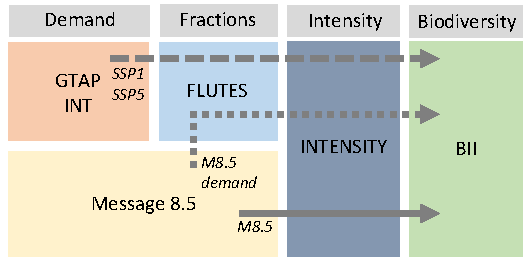
\includegraphics{chapters/figures/chapter4/fig_comparison.pdf}
    \caption{Diagram illustrating how each model component was applied to compare our predictions with Message 8.5. To make predictions under the SSP1 and SSP5 baseline scenarios (see \Cref{scenarios}), we estimated land-use demand from our CGE model (GTAP INT), downscaled projected land-use demands in our land-use model (FLUTES) and predicted land-use intensity and biodiversity intactness (BII) (dashed line). In Message 8.5 scenarios, we predicted land-use intensity and BII using land-use maps produced under the Message 8.5 model (solid line, M8.5 scenario) and extracting the demands of the Message 8.5 predictions, but downscaling these with FLUTES (dotted line, M8.5 demand).}
    \label{ch4:fig_comparison}
\end{figure*}


\subsection{Scenarios}
\label{scenarios}
We considered two baseline scenarios SSP1 \citep{fricko_marker_2017} and SSP5 \citep{kriegler_fossil-fueled_2017}, which together represent a wide range of possible future socio-economic conditions (\Cref{ch4:tab_oneill}). SPP1 is the ``taking the green road" scenario. In this pathway, the world slowly becomes more sustainable, respecting planetary boundaries \citep{downing_matching_2019, marquardt_identifying_2021}, and ensuring more inclusive and equitable development, with a commitment to achieving sustainable development goals \citep{riahi_shared_2017}. SSP5 is the ``taking the highway" scenario. In this pathway, the world is increasingly characterized by competitive, globally integrated markets, with rapid technological growth and the development of human capital. This global push for social and economic development results in fast global economic growth and the adoption of resource and energy-intensive lifestyles worldwide. Local environmental issues are managed successfully and there is a strong belief in the ability to effectively manage and engineer social and ecological systems \citep{riahi_shared_2017}. Radiative forcing levels under baseline SSP1 approximately correspond to RCP4.5 and under baseline SSP5 to RCP8.5 \citep{riahi_shared_2017}.

\begin{table}[]
\centering
\caption{Economic, policy, technology and environmental dimensions of SSP1 and SSP5 chosen in this analysis. Table adopted from Tables 2 and 3 in \citep{oneill_roads_2017}. LIC: low-income countries, MIC: medium-income country, HIC: high-income country.}
\label{ch4:tab_oneill}
\begin{tabularx}{\textwidth}{lYY}
SSP dimensions & SSP1 & SSP5 \\
\toprule
\textbf{Economy} &  &  \\
\bottomrule
Economic growth & High in LICs and MICs, medium in HICs & High \\
Inequality & Reduced across and within countries & Strongly reduced (mostly across countries) \\
International trade & moderate & High, with regional specialization in production \\
Globalization & Connected markets, regional production & Strongly globalized, increasingly connected \\
Consumption \& Diet & Low growth in material consumption, low-meat diets & Status consumption, meat-rich diets \\
 &  &  \\
\textbf{Policy} &  &  \\
International Cooperation & Effective & Effective for development goals, limited for environmental goals \\
Environmental Policy & Improved management of local and global issues, tighter regulation of pollutants & Focus on local environment with obvious benefits to well-being, little concern with global problems \\
Policy orientation & Toward sustainable development & Toward development, free markets, human capital \\
Institutions & Effective at national and international levels & Increasingly effective, oriented toward fostering competitive markets \\
 &  &  \\
\textbf{Technology} &  &  \\
Development & Rapid & Rapid \\
Transfer & Rapid & Rapid \\
Energy technology change & Directed away from fossil fuels, toward efficiency and renewables & Directed toward fossil fuels; alternative sources onot actively pursued \\
Carbon intensity & Low & High \\
Energy intensity & Low & High \\
 &  &  \\
\multicolumn{2}{l}{\textbf{Environment}} &  \\
Fossils & Preferences shift away from fossil fuels & No constraints \\
Environment & Improving conditions over time & Highly engineered approaches, successful management of local issues \\
Land Use & Strong regulations to avoid environmental trade-offs & Medium regulations leaed to slow decline in the rate of deforestation \\
Agriculture & Improvements in agricultural productivity; rapid diffusion of best practices & Highly managed, resource-intensive; rapid increase in productivity \\
\bottomrule
\end{tabularx}
\end{table}

To quantify the impact of using our land-use type/intensity models rather than those from Message 8.5, we also predicted land-use type/intensity and biodiversity intactness using land-use maps produced by the Message 8.5 IAM, available through LUH1 \citep[][\Cref{ch4:fig_comparison}]{hurtt_harmonization_2011}. In the M8.5 scenario, we directly used these future maps to estimate biodiversity \citep[analogous to][]{newbold_global_2015}. In the M8.5 demand scenario, we extracted only the land-use demands from the LUH1 maps. We then used FLUTES to allocate these demands to evaluate our model's ability to reproduce the spatial patterns of land-use change predicted by Message 8.5.

In all scenarios, we applied the same land-use intensity models to arrive at future maps of land-use type/intensity as input to biodiversity predictions (\Cref{ch4:fig_comparison}).


\subsection{Projecting changes in land demand}
Our CGE model GTAP INT is based on the GTAP 9 data base which collates census data on 137 economic regions across 57 commodity sectors \citep{aguiar_overview_2016}. The model is parametrized through input-output-tables that represent the inputs each economic sector requires for the production of outputs to meet domestic and international commodity demands of households and governments, which in turn are affected by prices and therefore supply. Commodity sectors are linked within and between regions, allowing for the propagation of economic impacts regionally and globally. In each region, commodities are produced and sold to domestic and foreign governments and households. In turn, households generate income from selling input factors (capital, labour, land) and governments through taxes \citep{kapitza_assessing_2021}. We aggregated the spatial resolution of our model to 30 world regions \citep[][see \Cref{apx:ch4:gtapaggr} for a list of regions and \Cref{ch4:fig_regionmap}b for a global map of the 30 regions]{van_ha_building_2017}.

8 of the 57 commodity sectors (7 crop sectors and livestock raising, see \Cref{ch4:tab_comms}) drive the requirement for land as primary factor of production. In GTAP INT the total land area (land endowment) from which land is allocated across these sectors can be changed in the baseline. Therefore, land supply that can be used for agricultural production is not fixed as in most other GTAP models and changes to the total land area are conceptually possible (instead of perfect substitutions of land area between different crop types, overall changes to the area under cropland are possible). Changes in land endowments within GTAP INT are calculated relative to the baseline supply by converting the relative changes in land endowments to absolute changes in cropland. This was achieved by using each commodities' harvested area in 2019 for a sector-wise weighting of the mean relative change of land endowed to the cropland class as a whole \citep[][see \Cref{apx:ch4:tab_faoharvested} for the relative weight of each sector]{kapitza_assessing_2021}.

\begin{table}[htb]
\centering
\caption{GTAP 9 commodity sectors we linked with cropland (1-8) and pasture land (9) \citep{aguiar_overview_2016}.}
\label{ch4:tab_comms}
\begin{tabularx}{\textwidth}{llY}
\toprule
& Code & Description\\
\bottomrule
1 & pdr & Paddy Rice: rice, husked and unhusked \\
2 & wht & Wheat: wheat and meslin \\
3 & gro & Other Grains: maize (corn), barley, rye, oats, other cereals \\
4 & v\_f & Veg \& Fruit: vegetables, fruitvegetables, fruit and nuts, potatoes, cassava, truffles, \\
5 & osd & Oil Seeds: oil seeds and oleaginous fruit; soy beans, copra \\
6 & c\_b & Cane \& Beet: sugar cane and sugar beet \\
7 & pfb & Plant Fibres: cotton, flax, hemp, sisal and other raw vegetable materials used in textiles \\
8 & ocr & Other Crops: live plants; cut flowers and flower buds; flower seeds and fruit seeds; vegetable seeds, beverage and spice crops, unmanufactured tobacco, cereal straw and husks, unprepared, whether or not chopped, ground, pressed or in the form of pellets; swedes, mangolds, fodder roots, hay, lucerne (alfalfa), clover, sainfoin, forage kale, lupines, vetches and similar forage products, whether or not in the form of pellets, plants and parts of plants used primarily in perfumery, in pharmacy, or for insecticidal, fungicidal or similar purposes, sugar beet seed and seeds of forage plants, other raw vegetable materials \\
9 & ctl & Cattle: cattle, sheep, goats, horses, asses, mules, and hinnies; and semen thereof \\
\bottomrule
\multicolumn{3}{Y}{Table adopted from https://www.gtap.agecon.purdue.edu/databases/contribute/detailedsector57.asp.}
\end{tabularx}
\end{table}
 
 In GTAP INT population growth cannot be accounted for explicitly, even though it is a principal driver of future socio-economic conditions. For this reason, we can currently only provide a partial SSP parametrization which focuses on the climate damages in terms of RCP that we expect to see under baseline SSP (SSP without mitigation). We assumed that climate damages are likely to contribute the majority of economic impacts of different SSP. Radiative forcing under baseline SSP1 approximately corresponds to RCP4.5 and radiative forcing under SSP5 to RCP8.5 \citep{riahi_shared_2017}.
 
 We quantified economic damages by first simulating trajectories of global warming under both RCP from the online simulation tool \textit{liveMAGICC} based on the general circulation model MAGICC6 \citep[Model for the Assessment of Greenhouse Gas Induced Climate Change][]{meinshausen_emulating_2011}. We then included these global warming trajectories in GTAP INT by applying environmental damage functions described in depth in \citet{roson_estimation_2016} and implemented in \citet{kapitza_assessing_2021}. Applying environmental damage functions in GTAP INT introduces shocks to land supply and agricultural and labour productivity. Decreases in land and labour productivity negatively affect the production of agricultural commodities. The heterogeneous impacts of climate change on different commodities are then reflected in changing prices to balance supply and demand. As a result, domestic products may be substituted by imports, with according changes in land endowments required to maintain domestic production \citep{kapitza_assessing_2021}.

\subsection{Spatially downscaling changes in land endowments}

We used a global fine-resolution (5 arcmin) land-use map for 2020 as the initial time step of our predictions. This map is available as part of the LUH1 data set \citep{hurtt_harmonization_2011} and is aligned with the land-use classes recorded in the PREDICTS data base we used to build biodiversity models \citep{hudson_predicts_2014}. Land-use classes were cropland (land used for cropping), pasture (land used for grazing of livestock), primary habitat (undisturbed natural habitat), secondary habitat (previously disturbed and recovering habitat), and urban land (dense urban settlement) \citep{hoskins_downscaling_2016}.

We applied FLUTES land-use model to spatially downscale the relative changes in land demand for each of the 30 regions. The model's advantage over other land-use models is that it can be readily implemented in R via the \texttt{flutes} GitHub package and is capable of directly modelling fractional land-use, instead of relying on land-use categories. A continuous representation of land use delivers higher information content than a categorical land-use classification because information on the sub-pixels about different land uses within the pixel is retained in the data set \citep{seo_mapping_2016}.

Similar to other land-use models \citep[i.e.][]{fuchs_high-resolution_2013, veldkamp_clue_1996}, FLUTES uses a set of climatic and socio-economic drivers to determine the suitability of the landscape for different land-use types (see \Cref{ch3:tab3} for the chosen drivers of land-use suitability). The suitability model in FLUTES is a multinomial model which assesses suitability of each land-use class relative to the suitability of other classes, therefore implicitly accounting for competition between different land-use types. We fitted separate suitability models for each of the 30 regions (see \Cref{ch4:fig_regionmap}a for a map of regions). In each region, we removed highly correlated covariate pairs, always keeping the covariate with the lower correlation with other covariates to maximise independent information retained in the final covariate set \citep{kapitza_assessing_2021}.

FLUTES applies a constraint in which the new establishment of a land use in areas where it was not historically observed is restricted to only a few cells \citep{kapitza_predictive_2020}. We used historic LUH1 time series maps (1990-2013) to determine the historically observable amount of cells (expressed as percentage of cells) that were completely devoid of a particular land-use type in a given time step but contained that land-use type in the next time step (\Cref{apx:ch4:tab_newest}).

To link agricultural commodity sectors from GTAP INT with the appropriate land-use type, we converted projected changes in crop sector land endowments to changes in total area by using their respective contributions to the total harvested area in each of the 30 regions in 2019 (\Cref{apx:ch4:tab_faoharvested}). For each region, we derived a future values for total land demand by multiplying the current area under cropland (estimated from the observed land-use data) \citep{hoskins_downscaling_2016} by this weighted average, establishing a direct proportional link between sector-wise relative changes in land endowments and the required total land area, as shown in \citet{kapitza_assessing_2021}. We proportionally linked changes in land endowments to the livestock sector with changes in pastureland \citep{kapitza_assessing_2021}.

We allocated future trajectories of cropland and pasture demand under the two scenarios based on the GTAP INT projections. We estimated demand for urban land by extrapolating FAO estimates of urban population growth by 2050 \citep{fao_faostat_2017} to 2100, proportionally linking these changes with changes in total land area \citep{kapitza_assessing_2021}. Since only knowledge of changes in cropland, pastureland, and urban land demand could be inferred from GTAP INT projections and FAO population projections, the two residual classes primary and secondary habitat remained unallocated. To determine changes in these classes, we used the mean suitability of each class predicted by our land-use suitability model in each subregion. For example, when 20\% of the landscape was primary and secondary habitat, a mean suitability for primary habitat of 0.2 and a mean suitability for secondary habitat of 0.6 would result in 5\% of the landscape allocated to primary and 15\% to secondary land \citep{kapitza_assessing_2021}.

\subsection{Predicting land-use intensity}

Following the land-use intensity classification recorded in the PREDICTS data base, we further divided land-use fractions under the 5 land-use types into three different intensity classes minimal use, light use and intense use, resulting in 13 land use type/intensity classes \citep[][pasture and urban were divided into two intensity classes only, see \Cref{apx:ch4:tab_intensity} for land-use type/intensity classes]{hudson_predicts_2014}.

To achieve this, we followed the steps outlined in \citet{newbold_global_2015}. We first used the Global Land System (GLS) data set \citep{van_asselen_land_2012} to obtain a global mapping of 29 land systems, each describing combinations of vegetation cover with human uses in terms of livestock raising, crop production and urban uses. We resampled the data to match a coarser resolution of 0.5 degrees, producing fractional cover of each GLS class in each resulting larger grid cell. We assigned GLS classes to the 13 land-use type/intensity classes. On cells where several GLS classes were linked to the same land-use type/intensity class, we summed the GLS-derived fractions, thus converting 29 GLS fractions to 13 land-use type and intensity fractions on each grid cell (see \Cref{apx:ch4:tab_glsmapping} for the links between GLS and land-use type/intensity classes). We aligned this GLS-derived map of land-use type/intensity fractions with the LUH1 data set's 2020 time step (available at the same spatial resolution of 0.5 degrees) by determining how much of the land-use types present in each LUH1 grid cell fell under minimal, light, and intense use in the GLS-derived land-use type/intensity map. LUH1 classes did not always overlap with a matching GLS class on every cell, resulting in missing information on use intensity in some cells. Where this was the case, the GLS map took precedence and we assumed that the land-use type in question was not present, proportionally increasing the land-use type and intensity fractions of the remaining classes.

To downscale the resulting 0.5-degree map of land-use type/intensity to 5 arcmin, we built binomial Generalized Additive Models (GAM) of cell-level intensity within each land-use type, using \texttt{R}-package \texttt{mgcv} \citep{r_development_core_team_r_2008, wood_fast_2011}. To build binomial models, we first converted intensity fractions within each land-use type to integer counts through multinomial draws \citep[see \Cref{ch3},][]{kapitza_predictive_2020}. Within each land-use type, integer counts representing land-use intensities summed to 1000. For land uses with three intensity classes: minimal, light and intense (cropland, primary, secondary) we built two models: 1) the probability of being minimal and the combined probability of being light and intense, and 2) when not minimal, the probability of being light. For land uses with two intensity classes light and intense (pasture and urban), we applied a single binomial model for the probability of being light and the probability of being intense.

Analogous to \citet{newbold_global_2015}, we modelled probabilities for different intensities within each land-use type as a function of population density and the respective land-use type, allowing estimated parameters to vary for each UN subregion to account for global heterogeniety in the modelled relationships. The model for the binomial probability of land-use intensity being minimal took the form

\begin{equation}
\begin{split}
logit(P_{minimal,k,i}) = \alpha_{k, \texttt{un}_i} + f_{1,k}(\texttt{pop}_{k,i}) + f_{2,k}(\texttt{lu}_{k,i})  + f_{3,k}(\texttt{lu}_{k,i}) * \beta_{k, \texttt{un}_i} \\ 
+ f_{4,k}(\texttt{pop}_{k,i}) * \gamma_{k, \texttt{un}_i}
    \end{split}
    \label{ch4:eq_fminimal}
\end{equation}

The model for the binomial probability of land-use intensity being light or intense, if it was not minimal, took the form

\begin{equation}
\begin{aligned}
\begin{split}
logit(Q_{light,k,i}) = \alpha_{k, \texttt{un}_i} + f_{1,k}(\texttt{pop}_{k,i}) + f_{2,k}(\texttt{lu}_{k,i}) + f_{3,k}(\texttt{lu}_{k,i}) * \beta_{k, \texttt{un}_i} \\ 
+ f_{4,k}(\texttt{pop}_{k,i}) * \gamma_{k, \texttt{un}_i}
\end{split}
\end{aligned}
\end{equation}

where \(P_{minimal,k,i}\) is the binomial probability of the intensity of land use \(k\) to be minimal, \(Q_{light,k,i}\) is is the binomial probability of the intensity of land use \(k\) to be light when not minimal, \(f_x()\) denotes a penalised spline fit, \(\texttt{lu}_{k,i}\) are the fractions of the land-use class for which intensity is being modelled, \(\texttt{pop}_{k,i}\) is population density \citep{gao_global_2020} and \(\texttt{un}_{i}\) are the United Nations subregions by which we allowed the model terms to vary \citep{newbold_global_2015}.

Accordingly, the overall fraction of being light, if not minimal, was:

\begin{equation}
\begin{aligned}
 P_{light,k,i} = Q_{light,k,i} * (1 - P_{minimal,k,i})
\end{aligned}
\end{equation}

The overall fraction of being intense was:

\begin{equation}
\begin{aligned}
P_{intense,k,i} = 1 - P_{light,k,i} - P_{minimal,k,i}
\end{aligned}
\end{equation}

The calculated probabilities for the different intensity classes sum to 1 for each land-use type. Accordingly, by multiplying land-use type fractions with the predicted probabilities for each intensity class, each land-use type is further divided into intensity classes without changing the total fraction of land under the according land-use type.

We estimated GAM parameters on a high performance computer on 10 parallel cores. We used the estimated parameters to downscale the land-use type/intensity map from 0.5 degrees to a resolution of 5 arcmin, by applying the modelled parameters to a 2020 map of population density \citep{gao_global_2020} and the 2020 LUH1 time step. We assumed the resulting map of land-use type/intensity at 5 arcmin as the present time step 2020 for our simulations. To predict future land-use type/intensity maps, we applied the modelled GAM parameters to the SSP1 and SSP5 land-use predictions we produced in FLUTES and future maps of global population density under SSP1 and SSP5 \citep{gao_global_2020}. We also applied the intensity models to the future land-use maps of the validation scenarios M8.5 and M8.5 demand.

\subsection{Predicting biodiversity intactness}

The PREDICTS data base currently contains 3,250,404 records of over 47,000 species from more than 26,000 sites that span all of the earth's terrestrial biomes \citep{hudson_database_2017}. A land-use record following the land-use type/intensity classification applied in this study exists for most sites.

To measure biodiversity change, we predicted and mapped present and future BII \citep{scholes_biodiversity_2005}. BII is ``the average abundance of originally present species across a broad range of species, relative to abundance in an undisturbed habitat" \citep{newbold_has_2016}. With the data available through the PREDICTS data base, it is possible to calculate BII directly by estimating abundance and richness at each site and comparing it to abundance and richness we would expect on pre-industrial, undisturbed habitat \citep{newbold_has_2016, de_palma_calculating_2019}. Given the impact of land-use changes on biodiversity, it can be expected that for each habitat characterized by different land-use type/intensities there exists a different number of individuals that belong to species that were already present before the habitat was disturbed. Theoretically, truly undisturbed habitat only existed before global industrialization. Since data from that time is unavailable, reference populations can be more practically estimated on currently existing sites that are virtually undisturbed. To estimate biodiversity intactness from the PREDICTS data base, we assumed that all sites that are recorded as minimally used primary habitat (primary minimal) host these reference populations \citep{newbold_global_2015}.

To ensure compatibility with previous work, we followed steps outlined in \citet{de_palma_calculating_2019} with minor adjustments \citep[also applied in][]{newbold_has_2016}. We first calculated total abundance at each PREDICTS site as the sum of all individuals sampled at each site, using effort-corrected estimates of abundance. Since there is variation in how abundance is measured between studies, we rescaled site-level abundance measures by dividing by the maximum sampled abundance within the same study, thus scaling abundance between 0 and 1 within each study \citep{de_palma_calculating_2019}. In doing so, we made abundance comparable between studies. To model the effect of land-use type/intensity on abundance, we built a linear mixed effects model of square-root rescaled abundance, using package \texttt{lme4} \citep{bates_fitting_2015}:

\begin{equation}
\begin{aligned}
\sqrt{A_{i, j}} = \alpha + \beta_{\texttt{lu}_{i, j}} + u_{j} + \varepsilon_{i,j} \\
u_{j} \sim \mathcal N(0, \sigma_u^2), \quad \varepsilon_{i,j} \sim \mathcal N(0, \sigma^2)
\end{aligned}
\end{equation}

 where \(A_{i, j}\) is rescaled abundance at site \(i\) in study \(j\), \(\texttt{lu}_{i, j}\) is the land-use type/intensity class (factorial), \(u_{j}\) is the random effect of different studies to account for differences in sampling methods between studies, and \(\varepsilon_{i,j}\) the error term. To account for non-normal error structure in abundance data, we used a square-root transformation of total abundance \(A_{j,s}\). We predicted this model to derive predicted abundance for each land-use type/intensity level.

A measure of predicted abundance for each class relative to primary minimal only gives a partial picture of biodiversity intactness because it does not provide insight on how much of that predicted abundance can be attributed to species that were originally present before habitat conversion. Compositional similarity of each site with primary minimal land-use type/intensity provides a factor by which abundance can be weighted to obtain BII (abundance of originally present species).

We calculated compositional similarity between non-primary vegetation sites and primary minimal sites, using the asymmetric Jaccard Index for Abundance \(J_a = \frac{UV}{V}\), where \(U\) is the summed abundance in the primary minimal site of the species found in both sites and \(V\) is the summed relative abundance in the non-primary vegetation site of all species in both sites \citep{newbold_has_2016, kunin_towards_1995}. To calculate the index, we counted the number of individuals per species at primary minimal sites and at sites containing other land-use type/intensity classes. The proportion between the number of individuals of a species at each site and the number of individuals of those species in the primary minimal site of each pair is the measure of compositional similarity. This calculation must be carried out for observations made within the same study, because otherwise the calculated index would also measure similarity between studies.

The model for compositional similarity took the form

 \begin{equation}
\begin{aligned}
logit(S_{i, j}) = \alpha + \beta_{\texttt{clu}_{i, j}} + \gamma * \log_{10} \texttt{dis}_{j} + \varepsilon_{i,j} \\
u_{j} \sim \mathcal N(0, \sigma_u^2), \quad \varepsilon_{i,j} \sim \mathcal N(0, \sigma^2)
\end{aligned}
\end{equation}

 where \(S{i, j}\) is compositional similarity at site \(i\) in study \(j\), \(\texttt{clu}_{i, j}\) is the land-use type/intensity contrast to the reference class primary minimal (factorial), \(u_{j}\) is the random effect of different studies to account for differences in sampling methods between studies, and \(\varepsilon_{i,j}\) the error term. To account for boundedness of compositional similarity between 0 and 1, we logit-transformed calculated compositional similarity \(S_{i,j}\). We predicted this model to derive predicted total compositional similarity for each land-use contrast to primary minimal.

Due to the random effects in the two models, the predicted values for abundance and similarity for each level are without dimension and have to be interpreted relative to other levels. Therefore, we divided the predicted values for each land-use type/intensity level by the predicted abundance and similarity for primary minimal to obtain abundance and compositional similarity relative to the baseline class.

We derived area-weighted maps of total abundance and compositional similarity by multiplying each fractional map of land-use type/intensity with the respective modelled estimate of mean abundance and similarity for each class. We mapped biodiversity intactness as the product of the two resulting maps.

\section{Results}

\subsection{Biodiversity intactness by biogeographic realm}
We analysed biodiversity intactness change under each scenario and modelling approach by biogeographic realm, aggregating spatial predictions of intactness to realm-wise means and interquartile ranges to characterise the range.

Mean changes in biodiversity intactness were small across bioegeographic realms, ranging from 0 to -1.5\% in SSP1 and 0 to -2.5\% in SSP5, although within realms, more extreme changes were predicted, especially in the Paleoarctic (indicated by large interquartile ranges in \Cref{ch4:fig_biodiv}a). Predicted changes under both scenarios were much smaller than those predicted under M8.5 and M8.5 demand, where mean changes in biodiversity intactness ranged from -2.5\% to -7\%. Results were similar between M8.5 and M8.5 demand, suggesting that the FLUTES model predictions about where and to what extent land use would change are comparable with those made by the land-use model applied in Message 8.5.

While predictions under M8.5 and M8.5 demand were approximately the same in their overall magnitude, there was some regional variation. Predictions under M8.5 resulted in more severe decreases of biodiversity intactness in the Neotropical and Indo-Malay realms than under M8.5 demand (\Cref{ch4:fig_biodiv}a, right two columns). Additionally, under M8.5 the models predicted a wider range of possible biodiversity intactness changes across the landscape in each realm except Oceania, as indicated by the wider interquartile ranges under this scenario. The Message 8.5 scenarios differed the most in their predictions for Oceania. Under M8.5 we predicted more severe decreases for this realm (-7\%) than under M8.5 demand (-2.5\%). Abundance (\Cref{ch4:fig_biodiv}b) and compositional similarity (\Cref{ch4:fig_biodiv}c) followed similar trends because they are proportional to intactness.

\begin{figure*}[htb]
  \centering
    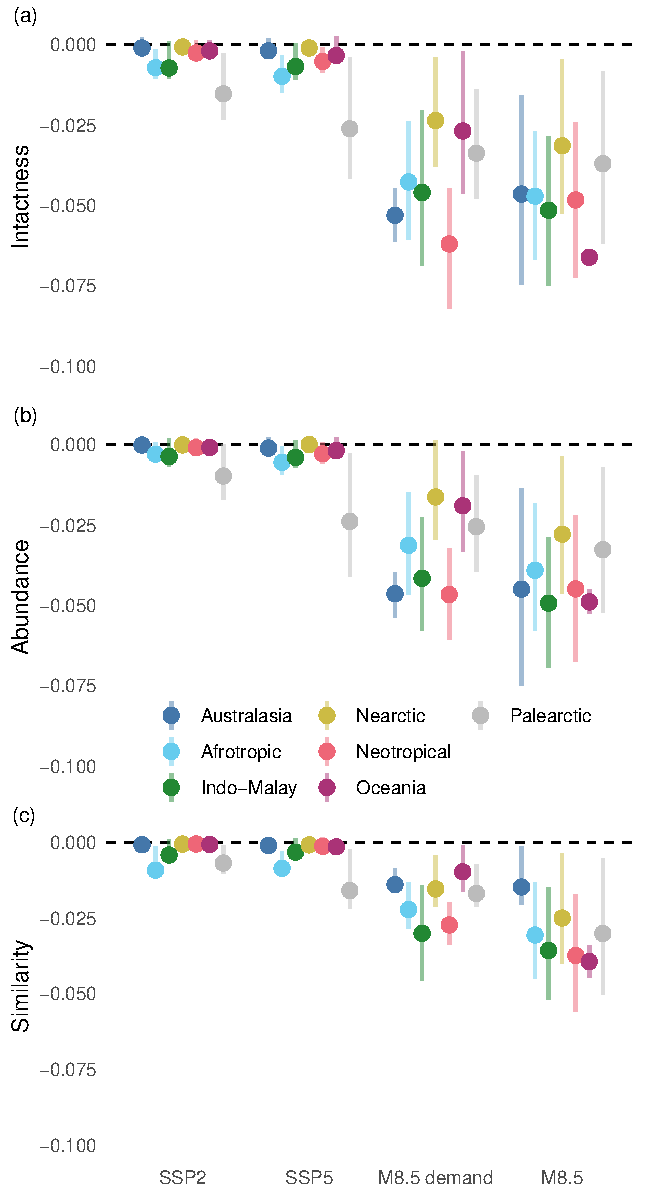
\includegraphics{chapters/figures/chapter4/fig_biodiv.pdf}
    \caption{Difference in (a) biodiversity intactness (\(\% / 100 \)), (b) abundance and (c) compositional similarity. We aggregated results by biogeographic realm \citep[see \Cref{ch4:fig_regionmap}b,][]{newbold_global_2015}. Bars indicate the interquartile ranges of cell-level changes within each realm.}
    \label{ch4:fig_biodiv}
\end{figure*}

\subsection{Biodiversity intactness by land-use type/intensity class}
Mean biodiversity intactness was predicted to be low for all intensities of cropland and pasture, as well as the urban intense class (ranging from 40\% to 70\%). The class with the lowest predicted mean intactness was cropland light (40\%), followed by cropland intense (55\%) and pasture light (60\%) \citep[\Cref{ch4:fig_biodivbyclass}, this finding is similar to][]{newbold_global_2015}. Particularly for cropland light and pasture light, low predicted mean intactness was due to low predicted relative compositional similarity (0.6 and 0.65 respectively), while abundance was predicted to be higher. Intactness was predicted to be highest on the primary light class, where it was \(>\) 100\%, due to abundance on this class predicted to be higher than the abundance in primary minimal. These results are in line with the direction and magnitude of the effect of each land-use type/intensity on abundance (\Cref{apx:ch4:fig_bdeffects}a for standardized effect sizes in the abundance model) and of each land-use type/intensity contrast on similarity (\Cref{apx:ch4:fig_bdeffects}b for effect sizes in the similarity model).

\begin{figure*}[htb]
  \centering
    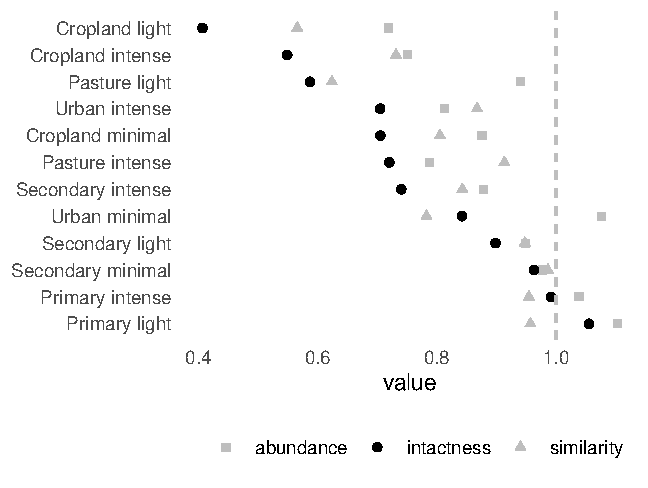
\includegraphics{chapters/figures/chapter4/fig_biodivbyclass.pdf}
    \caption{Calculated BII for each land use type/intensity class, including the underlying model predictions of abundance and similarity for each class. Values are relative to the undisturbed reference class primary minimal, which is indicated by the vertical dashed line through \(x=1\).}
    \label{ch4:fig_biodivbyclass}
\end{figure*}

\subsection{Biodiversity intactness by commodity sector}
The low predicted mean intactness on agricultural land-use types was linked with a negative effect of increases in agricultural land endowments on intactness. Global biodiversity intactness was negatively associated to increases in the wheat sector (\textit{wht}), followed by increases in cattle farming (\textit{ctl}), plant-based fibres (\textit{pfb}) and other crops (\textit{ocr}). Changes in land endowments to fruits and vegetables (\textit{v\textunderscore f}), as well as cane and beet (\textit{c\textunderscore b}), were positively associated with intactness. For other sectors oil seeds, paddy rice and other grains (\textit{osd, pdr and gro}), the determined effects of land endowment changes on intactness were very small. Due to the proportional linkage of intactness with abundance and similarity, the same effects were also observable for abundance and similarity (\Cref{ch4:fig_biigtap}a).

Effects differed between GTAP regions (\Cref{ch4:fig_biigtap}b). For example, we predicted a mean biodiversity intactness change of -6.6\% for Russia, which simultaneously had strong increases of up to 20\% in \textit{wht} and \textit{ocr} and decreases in \textit{v\textunderscore f} of approximately -4\%. At the same time, we predicted a mean intactness change in France of approximately +4\%, with simultaneous increases in \textit{wht} of 7\%. However, in France \textit{ctl} decreased by 5.5\%, which may have driven the increase in intactness. In Russia, \textit{ctl} decreased only by 2.4\% which was insufficient to offset the negative impacts of \textit{wht} and \textit{ocr} increases on intactness.

\begin{figure*}[htb]
  \centering
    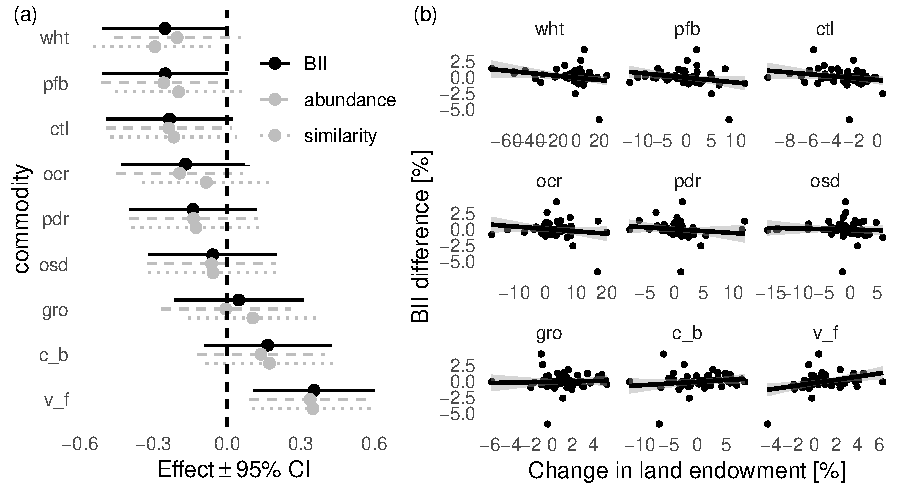
\includegraphics{chapters/figures/chapter4/fig_biigtap.pdf}
    \caption{Response of biodiversity intactness (BII) to changes in land endowments across sectors under SSP5. We determined trend lines with data from each GTAP region, using simple linear regression of intactness change against land endowment change, and calculated the effect of each variable on BII. The region with the highest increase in BII was France, the region with the highest decrease was Russia.}
    \label{ch4:fig_biigtap}
\end{figure*}

\subsection{Land endowment changes}
Predicted changes in land endowments under SSP1 were small overall \Cref{ch4:fig_gtap}, except for \textit{wht}, for which we predicted increases of approx. 5-10\% in all regions except Canada.
Under SSP5 we predicted more severe changes across sectors and regions. The strongest increases in \textit{wht} (as the commodity with the strongest negative effect on intactness) were predicted for Russia and Canada (approx. +19\%) under SSP5. The strongest decreases in \textit{wht} were predicted for Rest of South America and Sub-Saharan Africa with -34\% and -30\% respectively. The sector with the second strongest negative effect on intactness (\textit{ctl}) decreased the most in Canada and Indonesia under SSP5, with -9\% and -7\% respectively. In no region did \textit{ctl} increase under SSP5. The only increase in this sector could be observed under SSP1 in Russia, with \(<\) 0.5\%. \textit{c\textunderscore b} and \textit{v\textunderscore f}, which were associated with higher intactness, denoted increases in the majority of regions. Only in Europe, Canada, and China did \textit{c\textunderscore b} denote decreases.

\begin{figure*}[htb]
  \centering
    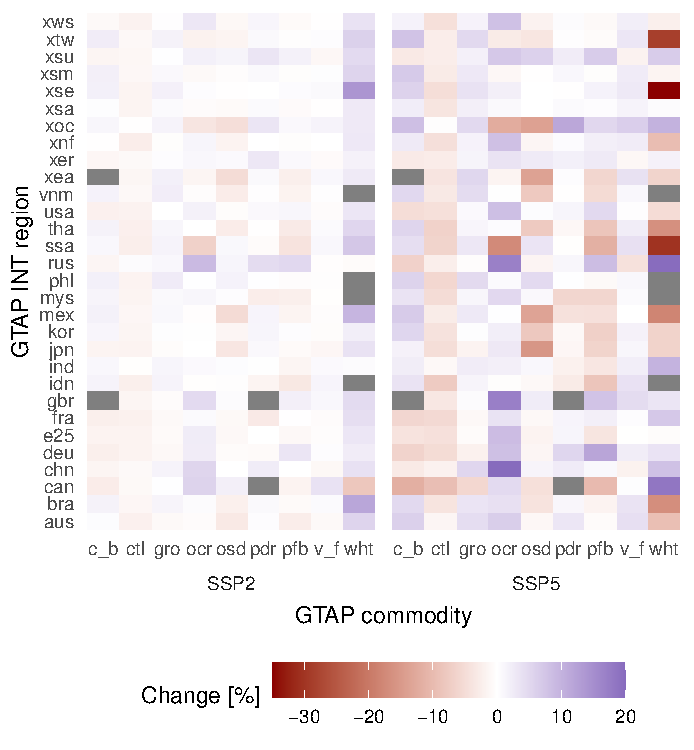
\includegraphics{chapters/figures/chapter4/fig_gtap.pdf}
    \caption{CGE model results. Sectors for which no harvested area was recorded in 2019 in a region (see \Cref{apx:ch4:tab_faoharvested}) are greyed out.}
    \label{ch4:fig_gtap}
\end{figure*}

\subsection{Land-use type/intensity}
Our predictions of global mean changes in fractional land use under SSP5 closely matched those made by the Message 8.5 model (M8.5 scenario) in cropland, pasture and urban, but our model predicted much higher global mean fractions of primary and much lower fractions of secondary habitat (\Cref{ch4:fig_landusecomp}a).

While spatial patterns of cropland and urban land were similar between models, pasture was predicted to be lower in SSP5 than in M8.5 throughout Australia, and to a lesser degree Central Asia and Southern parts of the African continent (\Cref{ch4:fig_landusemaps}). Predictions of primary habitat were higher in SSP5 across the Indo-Malay and Neotropical biogeographic realms but particularly in the Amazon catchment, the island of Borneo and in Papa New Guinea and Indochina. Predictions of secondary habitat were similar in our model compared to M8.5 in most regions, except for areas where primary habitat was predicted to be higher in our model. In these same regions, secondary habitat was predicted to be lower (\Cref{ch4:fig_landusemaps}), suggesting that differences in predictions of primary and secondary habitat between the models were caused by different approaches to predict primary and secondary habitats.

Land-use intensity predictions (which require predicted land-use type maps as input) were affected by these differences. Compared to Message 8.5, our model predicted substantially higher amounts of primary intense and primary light, and slightly higher amounts of primary minimal. In addition, our model predicted smaller amounts of pasture intense and across all secondary habitat intensities (\Cref{ch4:fig_landusecomp}b).


\begin{figure*}[htb]
  \centering
    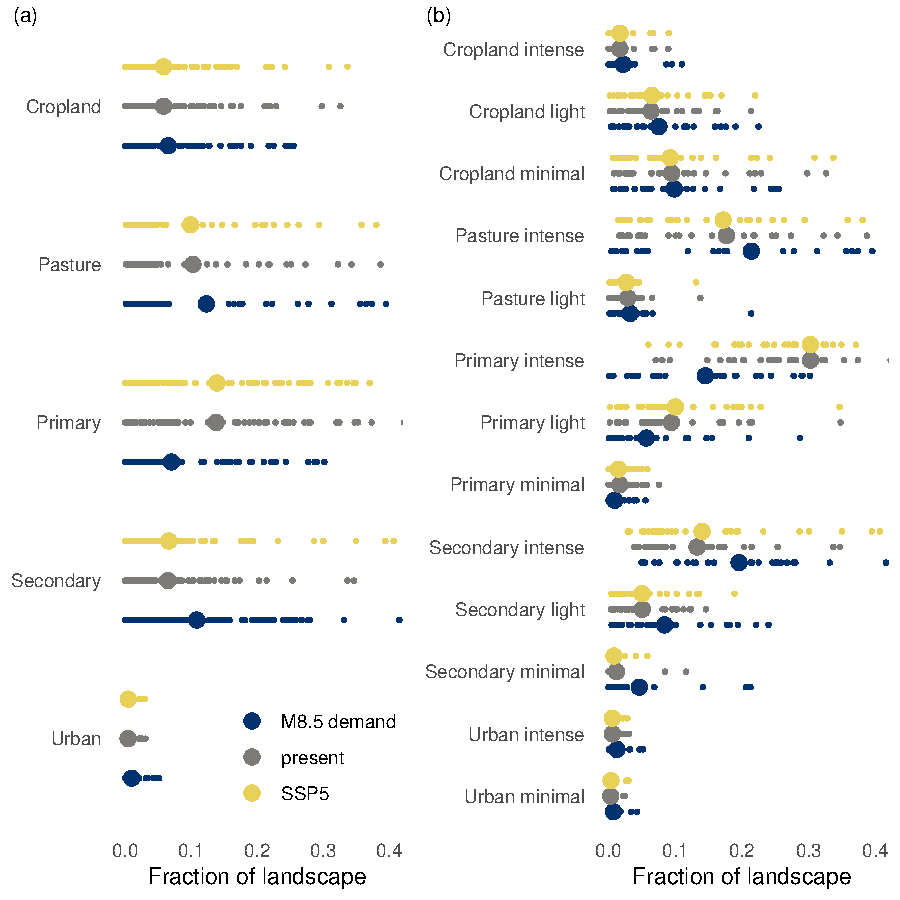
\includegraphics{chapters/figures/chapter4/fig_landusecomp.pdf}
    \caption{Comparison of global land-use predictions between SSP5 baseline and M8.5 validation scenarios. (a) Fractional cover of the five land-use types predicted by our models GTAP INT and FLUTES (SSP5 scenario) and predicted under Message 8.5 (M8.5 scenario). (b) Fractional cover of the 13 land-use type/intensity classes predicted from the SSP5 and M8.5 land-use type predictions, using our land use intensity model for both scenarios.}
    \label{ch4:fig_landusecomp}
\end{figure*}


\begin{figure*}[htb]
  \centering
    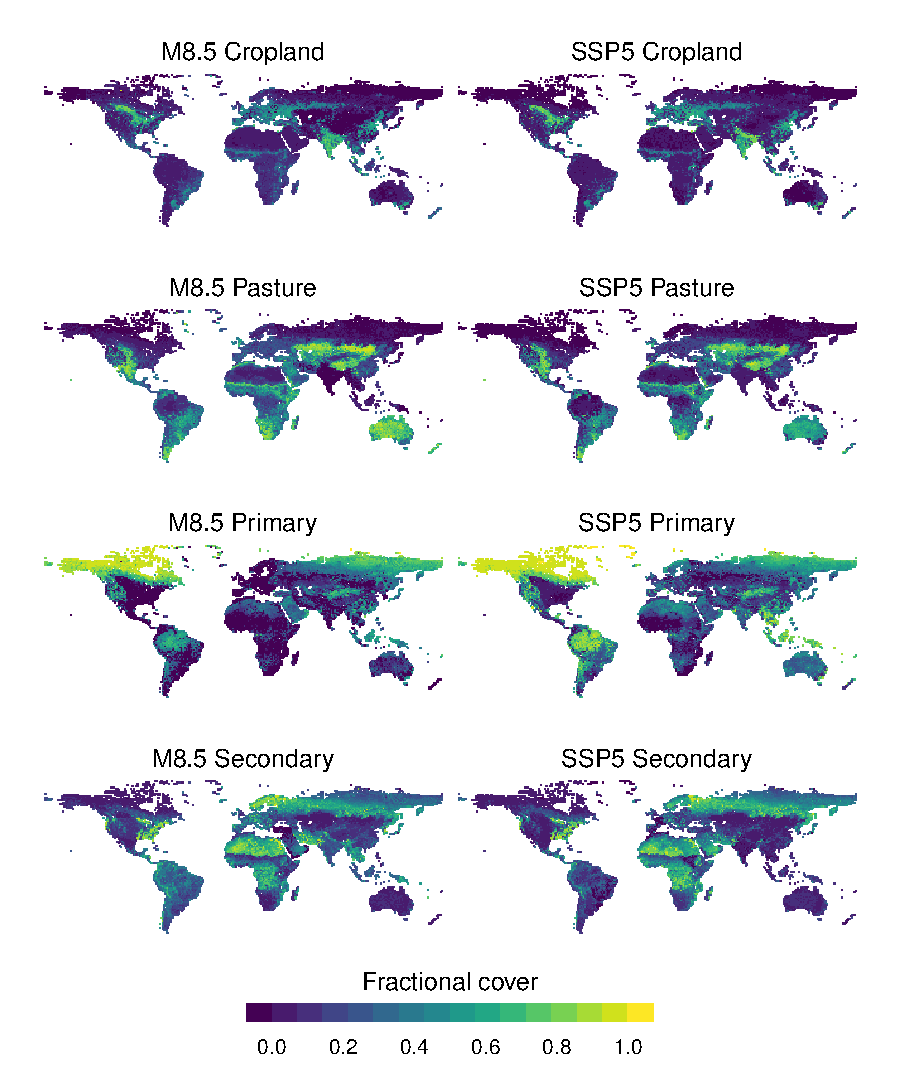
\includegraphics{chapters/figures/chapter4/fig_landusemaps.pdf}
    \caption{Predicted maps of four land-use types under M8.5 (the unaltered LUH1 maps) and the SSP5 scenario (projected using GTAP INT and FLUTES). Urban land predictions are not displayed because of very minor predicted differences between models.}
    \label{ch4:fig_landusemaps}
\end{figure*}

\section{Discussion}
In this chapter, we implemented new developments of our biodiversity assessment framework. We parameterized our CGE model to produce economic commodity demand predictions under two SSP, deployed a new fractional land-use model to predict land-use type/intensity changes under projected changes in agricultural land endowments and projected biodiversity intactness based on state-of-the-art models of biodiversity intactness. We compared our framework to the Message 8.5 model by making predictions about land-use change under two SSP scenarios and comparing results in terms of BII.

\subsection{Model choice strongly affects biodiversity intactness predictions}
We found that mean intactness changes were small across biogeographic realms in both SSP1 and SSP5, when compared to the intactness predictions made using Message 8.5. These smaller intactness losses predicted using our framework were primarily driven by relatively minor differences between the two models in predictions about the relative proportion of primary and secondary habitats remaining in the future, and even smaller differences in the predicted proportions of cropland and pastureland (\Cref{ch4:fig_biodivbyclass}).

Overall smaller changes to intactness predicted by our framework were the result of smaller areas predicted to go under cropland, pasture, urban intense and secondary intense land, and the larger areas predicted to remain under primary land secondary minimal (impact) land. Our predictions of cropland, pasture light, and urban minimal were only slightly smaller than those made under Message 8.5 for most classes. Among agricultural land-uses, only pasture intense was predicted to be notably smaller in SSP5 compared to Message 8.5 (\Cref{ch4:fig_landusecomp}b), though this had a minimal impact on intactness change predictions. These differences in predictions for land-use type/intensity classes between our framework and Message 8.5 were caused by differences in the respective predicted land-use type maps, because fractional land-use type was the only variable of the intensity models that was different between the frameworks (\Cref{ch4:fig_landusecomp}). The minor differences in the predictions for cropland and pastureland were probably driven by different agricultural commodity demands projected using our GTAP implementation when compared to the demand projections of the MACRO model in Message 8.5. However, we were unable to verify this because we could not obtain Message 8.5 projections for individual agricultural commodities.

The small changes in cropland predicted by our model were due to substitutions of land endowments between crop sectors. For example, there were substantial decreases in the wheat sector in about two thirds of the regions under SSP5 that may suggest decreases in demand for cropland, given the sector's high overall weighting in this class in most regions of the world (see \Cref{apx:ch4:tab_faoharvested}). However, in many of these regions, decreases in land endowments to wheat were accompanied by increases in land endowments to other sectors that occupied similar fractions of the overall area under cropping. For example, this was the case in Australia, where land endowments to wheat were predicted to decrease by about 8\%, while other sectors that together occupied a similar fraction of cropland increased by comparable amounts, leading to very minor net changes in demand for cropland.

\subsection{Model assumptions for primary and secondary land allocation drive uncertainty}

In our modelling framework, primary and secondary land were not linked explicitly with commodity sectors. Therefore, the projections of our GTAP INT model could not inform on the demand for these two classes. Instead, we weighted the amount of area allocated to each of the classes by their average predicted suitability across the modelled landscape (individual simulations were made for each of the 30 GTAP regions). However, using this approach, we predicted much more primary and much less secondary land using our framework, than was predicted by Message 8.5. Given that SSP5 is the only pathway that leads to the business-as-usual RCP8.5 world \citep{zittis_business-as-usual_2021}, recent trends in changes of the global coverage of primary and secondary land may be indicative of future changes. When looking at recent land-use changes between 1990 and 2005, primary land coverage decreased from 10.8\% to 10.2\% of the terrestrial land mass, while secondary land coverage increased from 39.2\% to 44\%. Given that under SSP5 deforestation is regulated moderately and decreases slowly, this trend will likely continue to a certain degree (at least on portions of primary and secondary land that are forest) but weaken into the future. Future changes in both classes are possibly smaller than recently observed trends and also the changes predicted by Message 8.5, and may more closely resemble the smaller changes predicted by our land-use model.

Our results for primary and secondary land must also be seen in the context of our method to predict them. Our multinomial suitability model fits the parameters of individual socio-economic and biophysical drivers of land-use suitability for each land-use type relative to the predicted suitability of other classes \citep{kapitza_predictive_2020}. The model achieves this by fitting intercepts as the log-odds of each class relative to the reference class when all covariates are kept constant \citep{sun_multinomial_2017}. Therefore, intercepts in our model can be interpreted as the baseline probability of each land-use type, approximately representing each type's initial prevalence in the landscape. Predictions of our suitability model reproduced this prevalence because the intercepts are added in the predictions for each class. Consequently, the higher amount of primary land observable in the initial land-use map strongly influenced the predicted average suitability for primary land. This effect may also have been exacerbated by our use of auto-covariates for each land-use type that link predicted suitability to the initial land-use distribution (see \Cref{apx:ch4:fig_landuseeffects} for standardized effects of land-use drivers, including auto-covariates, on land-use suitability).

Other IAM apply advanced vegetation models that are capable of simulating changes between different vegetation types, even accounting for different stages of succession. For example, in Message 8.5 the agricultural sector is predicted by the Agro-Ecological Zoning - World Food System (AEZ-WFS) model framework, which interfaces with the Dynamic Integrated Model of Forestry and Alternative Land Use (DIMA) \citep{hurtt_harmonization_2011, riahi_rcp_2011, rokityanskiy_geographically_2007}, a model of forestry and bioenergy demand. In this model, forest-related land-use processes (reforestation for conservation, afforestation for carbon capture, deforestation for timber and agricultural expansion, including crops for bioenergy production) are modelled based on local land prices, forest conversion costs, and land productivity.

Even more level of detail in modelling vegetation and forest dynamics is provided by the MagPIE (Model of Agricultural Production and its Impact on the Environment) model \citep{dietrich_magpie_2019}, which, together with the CGE model REMIND (Regional Model of Investment and Development) \citep{hilaire_remind-magpie_2020}, forms the MagPIE-REMIND IAM framework. MagPIE explicitly models vegetation dynamics at the level of plant functional types, using the Dynamic Global Vegetation Model (DGVM) LPJmL \citep[Lund–Potsdam–Jena managed Land model ,][]{bondeau_modelling_2007, sitch_evaluation_2003}. In this model, vegetation composition and distribution in natural as well as agricultural systems are modelled in response to land-atmosphere flows of water and carbon. Some of the processes simulated in the model include photosynthesis, fire disturbance evapo-transpiration, and vegetation structure \citep{bondeau_modelling_2007}. Accounting for vegetation dynamics at this level of detail is unlikely to improve our ability to discriminate between primary and secondary habitat, because conversions from primary to secondary habitat are driven by agriculture and forestry. Nevertheless, detailed models of vegetation dynamics may be useful to provide more realistic discrimination between different natural habitat types when also considering the age structure of secondary habitat \citep[see for example][]{newbold_global_2015}.

Integrating models of vegetation dynamics into IAM requires significant methods development. For example, MagPIE-REMIND submodels, including LPJmL, are interfaced explicitly through equations, enabling accounting for feedbacks and interactions. This also increases the required computational capacity and human inputs to levels that are currently unfeasible for our modelling framework. A more feasible method to predict vegetation dynamics in the context of our framework may be provided by linking the primary and secondary land-use types with the forestry commodity sector of our GTAP INT model. For example, in Message 8.5, increases in forestry are assumed to lead to larger requirements for secondary managed forests as with according reductions in primary forest cover \citep{riahi_rcp_2011}. This would require analysis of the vegetation types contained in the primary and secondary land classes. Further, the characterization of regional forestry patterns would be required to determine impacts on forestry on different forest types, depending on the local forest policy context. Modelling recent historical rates of conversion from primary to secondary habitat (at a regional scale) could provide the necessary statistical information to properly characterize elasticities of change between primary and secondary habitat, allowing these to be more adequately characterized in future iterations of our framework. 

\subsection{Changes in some commodity sectors drive losses in biodiversity intactness}
Even though the predicted intactness changes were small for SSP1 and SSP5, we were able to gain valuable insights into the drivers of biodiversity change at the level of individual commodity sectors. Historic biodiversity loss has previously been attributed directly with increases in wheat, sugar cane, rice, maize, palm oil, coconut, cassava, rubber, and coffee \citep{chaudhary_land_2016}. Our sensitivity analysis of the impacts of changes in land endowments of individual agricultural sectors showed that growth in the wheat (\textit{wht}), plant-based fiber (\textit{pbf}), livestock raising (\textit{ctl}), and other crops (\textit{ocr}) was associated with lower intactness, while growth especially in sugar cane/beet (\textit{c\textunderscore b}) and fruits/vegetables (\textit{v\textunderscore f}) was associated with higher intactness. However, this positive association is likely due to the strong negative association of intactness with wheat. In some regions with \textit{c\textunderscore b} and \textit{v\textunderscore f} increases, we predicted simultaneous decreases in \textit{wht}, which had a high contribution to changes in the cropland class. In these regions, the significant decreases in \textit{wht} resulted in an overall decreasing area under cropland, which then drove intactness increases rather than the small increases in \textit{c\textunderscore b} and \textit{v\textunderscore f}.

\subsection{The value of a streamlined and transparent workflow}
Interdisciplinary assessment frameworks combining methods across disciplinary boundaries provide crucial decision support for agencies and organizations concerned with making robust future predictions of biodiversity change to inform global conservation policy. However, most existing integrated assessment frameworks are not designed for this purpose, because they have been developed primarily for use in the analysis of economic risks associated with climate change and climate change mitigation \citep[i.e.][]{hilaire_remind-magpie_2020}, without much regard for biodiversity. While many of these frameworks are well documented, their complex methods and extensive parametrization requirements make them difficult to penetrate by small research teams that aim to analyse biodiversity outcomes under considaration of socio-economic drivers of change. 

Our new streamlined and transparent framework combines macro-economic, land-use and biodiversity modelling power and we were able to demonstrate that interdisciplinary biodiversity assessments for fine-grained analyses of socio-economic impacts on biodiversity without reliance on land-use predictions produced by external IAM are now within reach to ecologists. 

This opens up a pletora of research options to assess future biodiversity change and characterize model and prediction uncertainty. For example, climate change mitigation policy plausible under combinations of SSP and SPA likely affects agricultural activity (biofuels) and forestry (carbon plantings) \citep{kriegler_new_2014, riahi_shared_2017}, with impacts on global land-use and biodiversity. International trade agreements have significant potential to alter the international flow of goods and services, thus driving consumption and production of agricultural commodities \citep{van_ha_building_2017}, with potentially severe impacts on biodiversity \citep{newbold_trouble_2019}.

\subsection{Outlook}
Science is in a reproducibility crisis \citep{open_science_collaboration_estimating_2015} and publication bias and reductions in research transparency have also affected ecology and evolution \citep{fidler_metaresearch_2017, fernandez-juricic_why_2021}. Our methods to model land-use and biodiversity change have been documented at a high level of detail and we published our code in online repositories \citep[][see also the code repository accompanying this thesis for all code written for this chapter]{kapitza_assessing_2021, kapitza_predictive_2020}. Parametrizing and running our CGE model still requires expertise in macro-economics, but work is underway to introduce macro-economic modelling to ecologists in order to share and allow easy adaptation of these methods. 

Given that our model differed from Message 8.5 the most in terms of its predictions for natural habitat types (primary and secondary), the perhaps most important future development of our framework is the creation of a more sophisticated vegetation dynamics component. This is particularly useful for the in-depth assessment of biodiversity impacts of climate change mitigation policy, in which afforestation, wetland/grassland conservation, and biofuel production may strongly affect biodiversity. Another important future development is the more complete parametrization of our GTAP model in terms of SSP narratives. In GTAP INT we assumed that population growth and economic growth were included through the parametrization of future climate change pathways (RCP) via environmental damage functions, which themselves were parametrized by applying socio-economic narratives. However, this approach is limited because we have not yet been able to simulate the impacts of different levels of global collaboration, dietary changes or energy markets, which are all crucial corner stones of future socio-economic conditions. Regardless, each of the two iterations of our framework so far has provided new levels of integration of macro-economic, land-use and biodiversity models designed specifically for the assessment of the impacts of socio-economic change and trade on biodiversity.

\section{Conclusion}
In this chapter we provided further developments to our framework by aligning our scenario assumptions with SSP, thus making a crucial step toward the integrated assessment of biodiversity within future narratives long adopted by the IAM community. The implementation of our framework in this chapter provides detailed insights on the response of biodiversity across biogeographic realms, land-use/intensity types, and individual commodities, bringing a new level of detail to biodiversity assessments. Our framework predictions for biodiversity intactness differed from predictions made using land-use maps created by an existing IAM, because our land-use model FLUTES predicted smaller changes of primary and secondary habitats. We identified that further developments should focus in particular on the correct estimation of conversions between primary and secondary habitat types. 

We demonstrated the global applicability of our framework for streamlined integrated biodiversity assessments that do not rely on the high parametrization and expertise requirements typically accompanying existing IAM. With our framework we bring integrated biodiversity assessments further within reach of ecologists who seek to analyse local-to-global biodiversity change under a wide range of future scenarios, including global socio-economic change, climate change mitigation, biophysical climate change impacts, and trade agreements.


\chapter{Discussion}\label{ch5}
\newpage

\section{Thesis synthesis}
This thesis provides the initial development and implementation of a new modelling framework integrating macro-economic, land-use, and biodiversity modelling to assess the impacts of future socio-economic change on global biodiversity.
The first iteration of our framework was a continental-scale assessment of synergistic climate and land-use impacts on more than 1000 bird species (\Cref{ch2}). With this work we showed that assessment of multiple socio-economic and biophysical drivers of biodiversity at very fine resolutions are feasible with modest computational and modelling infrastructure and expertise. This initial work unravelled some of the complex pathways through which climate change impacts biodiversity, including through direct biophysical changes and through changes to global commodity demand and supply. This demonstrated the utility of integrated assessment frame- works to simultaneously analyze multiple drivers, and improve predictions of biodiversity change. A crucial outcome was the identification and prioritisation of research priorities, in particular (i) improving our ability to predict land-use change in response to commodity demand change, (ii) making predictions at a global scale to better capture global exports of biodiversity impacts, (iii) parametrizing scenario assumptions in line with established future narratives \citep[the so-called ‘shared socio-economic pathways’,][]{oneill_new_2014}, and (iv) increasing the taxonomic scope of our biodiversity predictions to generalize biodiversity predictions (see \Cref{ch5:fig1}).


\begin{figure}[htb]
\centering
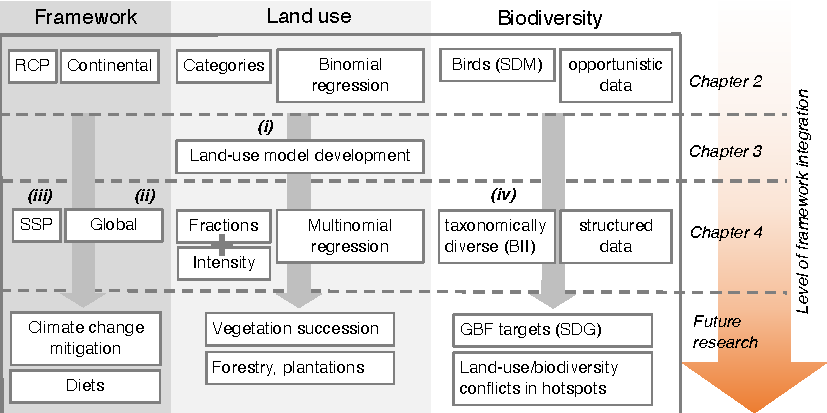
\includegraphics{chapters/figures/chapter5/fig1.pdf} 
\caption{Overview of developments accomplished in terms of scenario development, land-use and biodiversity modelling throughout this thesis. The second chapter identified research priorities (i-iv) that were tackled in subsequent chapters.}
\label{ch5:fig1}
\end{figure}

\subsection{Improving the land-use change model (i)}
\label{ch5:section_lumodel}
Following our initial study, we identified that the accessibility of our framework continued to be limited by the high parametrization requirements of the applied land-use model CLUE-S \citep{verburg_modeling_2002}. In CLUE-S, land-use elasticities (the propensity of land-uses to shift across the landscape in response to bottom-up processes, without changes to the overall occupied areas) are predominantly estimated subjectively. In addition, land-use suitability in the model is described using independent regression models for each land-use type, rather than allowing suitability to also be conditional on the predicted suitability of other land uses. The model is also limited by predicting fixed land-use categories, even though literature suggests that the fitting of downstream ecological models can be improved by using fractional land-use data, because fractional representations of land-use provide a higher level of sub-pixel information  \citep[\Cref{ch3}][]{bevanda_adding_2014, levers_drivers_2014, levers_drivers_2016}. 

To address these shortcomings, we developed a bespoke land-use model in \Cref{ch3} (`FLUTES'). We implemented our land-use model fully in the 'R' programming language \citep{r_development_core_team_r_2008}, thus ensuring accessibility for R-trained ecologists. Our land-use model implements land-use fractions to bring the representation of land-use further in line with the optimal requirements for downstream ecological models. We also developed a multinomial suitability model in which land-use suitability is modelled conditional on the suitability predicted for other land-use classes, thus implicitly providing parametrization of bottom-up processes affecting the location and magnitude of land-use change (competition between land uses). Compared to our implementation of CLUE-S, our model also improves the parametrization of land-use elasticity by using observed data to determine locations where a new land-use can be established without having been present historically.

\subsection{Increasing the spatial extent of analyses (ii)}
In \Cref{ch4} we provided a first global implementation of our framework and compared biodiversity change predictions made using our comparatively simple and streamlined framework to those provided by a large integrated assessment framework known as ‘Message 8.5’ \citep{riahi_rcp_2011}. Following an analysis pathway provided by \citet{newbold_global_2015}, we generated economic demand, land use and biodiversity predictions using with our intertemporal GTAP model ’GTAP INT’ and our land-use model ’FLUTES’. We then compared the biodiversity predictions derived using the two frameworks. Global predictions of agricultural land-use demands and their spatial realisation were predicted to be similar between the models, even though some more work is required to appropriately model and evaluate spatial predictions of primary and secondary forest habitats (see \Cref{ch5:section_lumodel}). Despite  this caveat, we were able to bring our framework to the global scale and found a comforting congruence of predictions, even though our model is far more streamlined, pattern-based and simple to use. This finding confirmed that our streamlined approach with minimal parametrization requirements is a tool that may allow IAM to be more widely used by a greater variety of agencies and organisations that seek integrated analysis of biodiversity outcomes in complex socio-ecological contexts.


\subsection{Scenario alignment (iii)}
In \Cref{ch4}, we further aligned our scenario parametrization with the SSPs \citep{oneill_new_2014} and provided the foundation for detailed assessments of climate change mitigation and trade. Using GTAP INT, we parametrized RCP8.5 with environmental damage functions. Since RCP forcing levels are emergent properties of SSPs, we assumed that our projection of economic damages under a given RCP approximates economic damages we would expect under a related SSP, also assuming that aspects of socio-economic change, such as gross domestic product (GDP) and population growth, are implicit in this parametrization. This assumption was necessary because adjusting population growth and GDP explicitly is not possible in GTAP INT. However, in our GTAP INT implementation, we applied climate damages of RCP8.5 in order to approximate SSP 5 and achieved similar predictions for agricultural land demand as predicted by Message 8.5. This suggests that our framework provides a good approximation to predictions made under established harmonized scenario assumptions. The GTAP INT model we applied in \Cref{ch4} is also an improvement over the GTAP INT model we applied in \citet{kapitza_assessing_2021} (\Cref{ch2}). In the previous iteration, we assumed a linear temperature increase to levels that correspond with scenarios we explored (RCP2.6 and and RCP8.5). In the more recent iteration, we directly included temperature trajectories as they were predicted for the RCP under the MAGICC6 model, without requiring linear interpolation. This results in a more realistic representation of future economic damages.

When analyzing other aspects of socio-economic change, it is crucial to account for RCP, population growth and GDP independently, because climate change mitigation strategies may lead to different combinations of socio-economic change with radiative forcing. For example, when the global policy response to mitigate climate change is highly fragmented, mitigation costs are high regardless of GDP and population growth, making it less likely that reductions in forcing levels and warming can be achieved \citep{kriegler_fossil-fueled_2017}. Accordingly, in order to explore scenarios of global climate change mitigation, RCP cannot always be used as a proxy for SSP and further scenario parametrizations will usually be necessary to properly parameterize an SSP.


\subsection{Increasing taxonomic scope (iv)}
In the initial iteration of our framework we applied models based on presence-only data, because these data are widely collected in opportunistic surveys and collated through the Global Biodiversity Information Facility (GBIF) database, making them readily available for modelling studies \citep{gbif_gbif_2016}. However, as for most other biodiversity data sampled in unstructured surveys, sampling bias remains a pervasive issue undermining the vast geographic, temporal and taxonomic coverage of the data base \citep{troia_filling_2016, kapitza_assessing_2021}. Even though methods exist to account for sampling bias, they tend to depend on the study context and lack coherent approaches that can be scaled up \citep{kramer-schadt_importance_2013, stolar_accounting_2015, kapitza_assessing_2021, fithian_bias_2015}.

Our applied species distribution models required at least 20 occurrence points to estimate relative likelihoods of occurrence and applying this filter for the countries chosen in the analysis, the only taxonomic group with sufficient (\(>\)1000) species satisfying this requirement was birds. An additional advantage of using bird species was that we could make simple assumptions about the realisation of predicted potential niches, because the ability to fly implies relatively unconstrained dispersal (we only constrained dispersal in Australia to adjacent bioregions) \citep{kapitza_assessing_2021}.

Changes in the geographic distributions of birds alone give an insufficient picture of biodiversity and the continental scope of the initial study limits the generalisation of findings to global geographic extents. To be able to assess human impacts on biodiversity at a global scale, it is necessary to maximise the representation of taxonomic diversity because impacts are heterogeneous across taxonomic groups \citep{hudson_predicts_2014}. Our GBIF-based method of stacking SDMs applied in \Cref{ch2} would have quickly caused data processing and modelling requirements to exceed the computing power available to me, given that the GBIF data base currently holds almost 1.5 trillion records for Animalia alone \citep{gbiforg_gbif_2021}. Given that we ran continental-scale SDMs for bird species on a high-performance cluster on 12 parallel cores and these computations took approximately 72 hours to complete, significant computational challenges would also have arisen during model building and prediction when upscaling the analysis to all taxa and to a global extent. 

To overcome these barriers, we based our biodiversity models on structured survey data from the PREDICTS database. The PREDICTS database allows for the calculation of macroecological indices that are based on effort-corrected abundance measures from structured surveys that cover 13 out of 14 biomes, 25 out of 35 biodiversity hotspots and 28000 species from various taxonomic groups, including plants, insects, amphibians, mammals, birds, and reptiles. For our research priority of providing global predictions of biodiversity change, the database provides an ideal alternative to GBIF, because quality-control and bias-accounting are part of the data collection and submission protocols \citep{hudson_predicts_2014}. Several authors have highlighted the additional benefits of using abundance-based metrics to evaluate biodiversity change \citep{scholes_biodiversity_2005, newbold_global_2015}.

With PREDICTS, we were quickly able to estimate and predict biodiversity intactness \citep{scholes_biodiversity_2005}, providing a simple approach to estimate a response of biodiversity to scenarios of socio-economic change with global coverage, accounting for both species richness and abundance. As the name suggests, the biodiversity intactness index provides an overall index of how biodiversity is anticipated to change with broadly changing land-use patterns.  The properties of the index have not been widely tested or evaluated against observed species level change in a variety of landscapes. There exists an opportunity to compare how a biodiversity intactness index analysis compares with an analysis of change based on species distribution models.

\section{Opportunities for improvement}

\subsection{Improving the biodiversity intactness model}
BII is a general index that cannot account for all important aspects of biodiversity change. A fundamental limitation is the exclusion of species-level information when estimating the underlying macroecological indices (abundance and similarity) from which BII is calculated. When this information is missing, it is not possible to track the status of endangered species. For example, this could lead to predictions of high intactness in biodiverse regions, where human impacts have historically particularly affected endangered species that already have experienced abundance declines. While impacts on these species may have been severe, they are not represented in BII \citep{martin_biodiversity_2019}. To predict localized impacts on many endangered species and derive optimal conservation policy, species distribution models are better suited because they can capture fine-scale variations in environmental space. Predictions of habitat suitability typically provided by SDM allow for the spatial prioritization of areas for conservation and restoration \citep{wilson_applying_2011}. The systematic selection of a small number of flagship species can even be an effective tool for efficient conservation prioritization representative of global biodiversity \citep{mcgowan_conservation_2020}.

Another limitation to the estimation of BII from the PREDICTS data base is posed by its reliance on a relatively coarse representation of land-use. \citet{martin_biodiversity_2019} criticized that global intactness trends predicted by \citet{newbold_global_2016} likely underestimated historic losses of biodiversity in tropical plantation forests and dense population centres, and overestimated biodiversity declines in semi-arid rangelands. Spatial patterns of biodiversity intactness and biomass intactness \citep{erb_unexpectedly_2018} can be expected to correlate in space. However, \citet{martin_biodiversity_2019} found that spatial patterns in these indices did not agree for many parts of the world, even exhibiting a strong negative correlation when measured across 32 biodiversity hotpots. Significant improvements to our framework may be achieved by matching land uses recorded in the PREDICTS data base to the more highly resolved Land Use Harmonization Project 2 (LUH2) database \citep{hurtt_harmonization_2020}. In LUH2, rangeland and pastureland are distinguished, allowing for a more discriminate modelling of the biodiversity response to these classes. Furthermore, superimposing global plantation maps \citep{harris_spatial_2019} would allow a much more discriminate mapping of forest types that each differ in their implications for biodiversity. Including adequate global land-use maps that are precise in terms of distinguishing habitats of different significance for biodiversity should remain a high priority in future developments of our framework, regardless of the applied biodiversity models.


\subsection{Improving FLUTES}

The approach to model land-use change we provide through our FLUTES model is based on statistical regression analysis and a simple allocation algorithm. We intentionally simplified our model to streamline parametrization requirements for the application in global biodiversity assessments (\Cref{ch3}). However, rangelands and pasturelands, as well as natural forests and plantation forests, are often observed within the same environments \citep[for example, semi-arid rangelands and pasturelands on the Australian continent, or natural forests and plantations in tropical regions, see][]{newbold_reply_2019}. Basing a land-use model almost entirely on regression methods (as done in FLUTES) that model observed patterns (including transitions) limits the ability of FLUTES to represent bottom-up processes that drive fine-scale land-use change patterns \citep{noszczyk_review_2019}. FLUTES could be made arbitrarily more complex and include arbitrarily many land-use classes and variables that predict their suitability. The challenge is finding the right level of complexity for the problem at hand. If a very fine-scale analysis of local land-use changes is required, it may be better to use a more mechanistic model such as LUTO \citep{bryan_supply_2014}, so that complex human behaviours that influence land-use change can be incorporated and analyzed.

Advances in computational capacity have increasingly allowed for the application of machine learning techniques, such as Artificial Neural Networks (ANN) in land-use change modelling \citep{noszczyk_review_2019, koomen_core_2011}. ANN are powerful tools to recognize patterns of change from observed land-use time series. They apply user-defined transition rules and predict transitions based on the relationship of historic land-use change patterns with a wide range of socio-economic and biophysical variables \citep{pijanowski_using_2002}.  The main advantage of ANN over our method is that finely resolved spatial information from entire historic time-series can be used to train networks. FLUTES also uses historic land-use time series, but the information is only used to constrain the model by limiting how much of a land use can be established where it was not historically present. This provides a less refined parametrization of the magnitude and location of transitions between land uses through time because observed spatial patterns are not taken into account.

Linking ANN with FLUTES may be possible, but some challenges remain. In order to achieve an information content in the final land-use map that at least matches the fractional maps produced by FLUTES (currently at 10km), predictions at an even higher spatial resolution of \(>\)10km would be required when parametrizing transitions between land-use categories, possibly leading to computational and data constraints at the global scale. Moreover, the non-linear relationships considered in ANN may lead to overfitted parameter estimates. Compared to logistic regression, this may lead to lower predictive performance when extrapolating into new environmental space \citep{dreiseitl_logistic_2002}.

Nevertheless, given the fine-scale dynamics of land uses that drive species habitat change and, consequently, biodiversity intactness, unsupervised learning methods that use historic land-use time series, such as ANN, have potential to significantly boost our framework's predictive capacity, when fitted and evaluated carefully.

\subsection{A streamlined and open integrated assessment framework to predict biodiversity}

The work in this thesis was driven by the need for integrated, cross-disciplinary approaches to biodiversity modelling \citep{ipbes_summary_2016, ipbes_summary_2019}. 

Established integrated assessment models (IAM) are typically designed for the assessment of economic transformation strategies to mitigate and adapt to climate change and as such provide little to no insight on biodiversity outcomes \citep{harfoot_integrated_2014}. In addition, by applying highly parametrized submodels that are developed and maintained by large research teams and backed through institutional support, they are prohibitively complex in an ecological research context. For this reason, adopting existing IAM for biodiversity assessments continues to be faced with significant barriers. 

Despite these limitations, biodiversity assessments applying at least some degree of cross-disciplinary model integration have been implemented recently, also including the first case study of this thesis \citep[\Cref{ch2},][]{kapitza_assessing_2021}. \citet{newbold_global_2015} provided a spatially-explicit assessment of global biodiversity intactness under future land-use changes predicted under the Message 8.5 model \citep{riahi_rcp_2011} and \citet{marques_increasing_2019} applied economic and land-use models to identify the extent to which economic teleconnections have led to remote, exported impacts of economic activity on avian diversity globally. More complete levels of integration between economic, land-use, and biodiversity modelling have been provided by \citet{leclere_bending_2020}, who use the land-use modelling components of several IAM to examine how to halt and reverse the decline of terrestrial biodiversity while simultaneously growing sufficient food for the world's growing human population. \citet{veerkamp_future_2020} use two established IAM to predict biodiversity and ecosystem services in a European context. \citet{kapitza_assessing_2021} assess biophysical and socio-economically mediated climate change impacts on bird species at continental scale by coupling a general equilibrium model with land-use and biodiversity models (\Cref{ch2}). 

Nevertheless, such examples of integrated biodiversity assessments remain rare and they also continue to be limited by their scalability to global extents, their coarse spatial resolutions preventing adequate representation of highly localised processes, and the extent to which their scenario assumptions are aligned with socio-economic narratives applied in other disciplines, such as climate science. Addressing this gap, we designed our framework to be accessible in ecological research environments, ensure high spatial resolutions at global scales and align model assumptions with future narratives already established in the IAM community.

Our framework also attempts to address the reproducibility crisis in science \citep{open_science_collaboration_estimating_2015}, which also affects ecology as a discipline \citep{fidler_metaresearch_2017, fernandez-juricic_why_2021}. We coded and documented our methods to model land-use and biodiversity change fully in \texttt{R} \citep{r_development_core_team_r_2008}, thus making our code accessible to a fast growing number of ecologists trained in R: \citet{lai_evaluating_2019} found that the share of studies published in 30 ecology journals that report \texttt{R} as primary tool for analysis has increased from 11.4\% in 2008 to 58\% in 2017, also highlighting the importance of \texttt{R} as a catalyst for open science and reproducibility. Our implementation of GTAP INT does not yet interface with R, but according developments are currently underway to address this shortcoming.

Moreover, our framework parametrization makes assumptions that significantly streamline the analysis and provide substantial reductions in model complexity compared to established IAM. For example, we linked 8 crop sectors to one cropland class and used the reported harvested area of each crop sector for a weighting of each sector's contribution to changes in the total area under cropland. This assumption derived similar results for changes in global cropland as were predicted by the Message 8.5 IAM (see \Cref{ch4}). However, there are trade-offs between reducing model complexity and causing increases in model uncertainty. For example, with our simplified assumption that the total amounts of primary and secondary habitats are driven by their respective modelled biophysical and socio-economic suitability, our framework produced different results than Message 8.5 (see \Cref{ch4}). While recent business-as-usual trends in conversion rates from primary to secondary habitat suggest that our predictions could be plausible, this difference between the predictions of the two frameworks also implies that our simplified assumptions may also increase model uncertainty. In order to identify differences and investigate whether they are due to unrealistic assumptions in the established IAM, or in our framework, it may be useful to compare predictions of our framework with predictions by established IAM, using baseline scenarios.

\subsection{A framework to measure progress toward Sustainable Development Goals}

Integrated assessment frameworks that combine methods across disciplinary boundaries enable us to account for complex interactions between human and natural drivers of biodiversity change, thus reducing uncertainty about the future. This also makes them important tools to inform sustainable policy-making \citep{veerkamp_future_2020, ipbes_summary_2019, un_general_assembly_transforming_2015}.
While some progress has been achieved toward the Aichi biodiversity targets, none of the targets could be fully achieved by 2020 and there is now an unprecedented need to act to protect biodiversity \citep{scbd_global_2020}. To slow down, halt and reverse business-as-usual declines of biodiversity is tightly intertwined with achieving the 2030 Agenda for Sustainable Development, directly contributing to the achievement of Sustainable Development Goals (SDG) 1, 11, 13, 14 and 15, which seek to combat poverty and climate change, build sustainable cities, and preserve terrestrial and marine life, and indirectly supporting SDGs 7, 8, 9 and 12, which seek to provide affordable and clean energy, economic growth, innovation and infrastructure, and responsible consumption and production \citep{un_general_assembly_transforming_2015, scbd_global_2020}. Steps toward achieving the goals are consistent with those outlined in the most recent assessment report of the Intergovernmental Science-Policy Platform on Biodiversity and Ecosystem Services (IPBES) \citep{ipbes_summary_2019} and include slowing down global warming, conservation, and restoration \citep[see also the current UN Decade on Ecosystem Restoration,][]{unep_resolution_2019}, further reducing the impacts of invasive species, pollution, and unsustainable exploitation and transformation of diets, and the production and demand of food. 

So far, our framework has enabled us to explore climate change and land-use change impacts driven by socio-economic change, making our methodology suitable to assess and monitor progress toward SDG from local-to-global scales. Our method could be well suited to analyse synergistic climate and land-use change impacts in the world's biodiversity hotspots under various future scenarios (SSP, climate change mitigation scenarios, scenarios isolating the impacts of dietary shifts), allowing us to quickly highlight policy options to protect some of the most vulnerable ecosystems. We have already paved the way to these kinds of analyses: our GTAP INT model has been rolled out for a 30-region representation of the world (\Cref{ch4}), our land-use model can be applied at fine resolutions anywhere in the world, and we have illustrated the application of a method to predict and map biodiversity change that is based on structured survey data covering 25 out of 35 biodiversity hotspots and 16 out of 17 megadiverse nations \citep{hudson_predicts_2014}.


\section{Concluding remarks}
With this framework, we contribute an open method to model socio-economic impacts on biodiversity, bringing integrated assessments of biodiversity change within reach of ecologists. While our framework is still in its early stages, the work presented in this thesis demonstrates that we are now capable of successful applications and have identified where developments are necessary to further improve our framework's relevance. First, future applications will see a particular focus on improving predictions of primary and secondary natural habitat types. Second, we will provide further integration with the scenario assumptions that are also applied in established IAM in order to maximize the policy relevance of our predictions of biodiversity change. Third, we will tailor our framework toward assessing impacts in biodiversity hotspots to quickly identify suitable measures to protect biodiversity in the world's most vulnerable regions. It is our hope that this work inspires comparable efforts and ecologists can soon choose from a much wider range of tools to help assess human impacts on biodiversity and monitor our progress toward a world in line with the 2030 agenda.

\clearpage{\pagestyle{empty}\cleardoublepage}

{
\backmatter
\chapter{References}
%\newpage
\bibliography{bibliography}
\clearpage{\pagestyle{empty}\cleardoublepage}
}

%---------------------------------------------------------- 
% APPENDICES
% include chapters as needed (will be numbered differently)
%---------------------------------------------------------- 
\let\svaddcontentsline\addcontentsline %supress tables and figures in index from showing
\renewcommand\addcontentsline[3]{%     % up in lists in frontmatter
  \ifthenelse{\equal{#1}{lof}}{}%
  {\ifthenelse{\equal{#1}{lot}}{}{\svaddcontentsline{#1}{#2}{#3}}}}

\clearpage
\appendix
\fancyhead[R]{\sc Appendix \thechapter}
\clearpage{\pagestyle{empty}\cleardoublepage}


\chapter{Supplementary Information Chapter 2}\label{apx:ch2}
\newpage


% Please add the following required packages to your document preamble:
% \usepackage{graphicx}
\begin{table}[htb]
\centering
\caption{Climate, other biophysical, and socioeconomic predictors used as initial input to bias model, SDM, and land use model. Predictor choices were made based on literature. The initial predictor sets were reduced using correlation analysis.}
\label{apx:ch2:tab1}
\begin{tabularx}{\textwidth}{lllllY}
\toprule
Short name & Long name & \multicolumn{3}{c}{Chosen?} & Source \\ \bottomrule
 &  & \multicolumn{1}{c}{Bias} & \multicolumn{1}{c}{SDM} & Land use &  \\
\textbf{} & \textbf{Climate predictors} & \textbf{} & \textbf{} &  & \citep{hijmans_very_2005} \\
\textit{bio1} & Annual mean temperature &  & x & x &  \\
\textit{bio2} & Mean diurnal range &  & x & x &  \\
\textit{bio3} & Isothermality &  & x & x &  \\
\textit{bio4} & Temperature seasonality &  & x & x &  \\
\textit{bio5} & Maximum temperature of warmest month &  & x & x &  \\
\textit{bio6} & Minimum temperature of coldest month &  & x & x &  \\
\textit{bio7} & Temperature annual range &  & x & x &  \\
\textit{bio8} & Mean temperature of wettest quarter &  & x & x &  \\
\textit{bio9} & Mean temperature of driest quarter &  & x & x &  \\
\textit{bio10} & Mean temperature of warmest quarter &  & x & x &  \\
\textit{bio11} & Mean temperature of coldest quarter &  & x & x &  \\
\textit{bio12} & Annual precipitation &  & x & x &  \\
\textit{bio13} & Precipitation of wettest week &  & x & x &  \\
\textit{bio14} & Precipitation of driest week &  & x & x &  \\
\textit{bio15} & Precipitation of driest month &  & x & x &  \\
\textit{bio16} & Precipitation of wettest quarter &  & x & x &  \\
\textit{bio17} & Precipitation of driest quarter &  & x & x &  \\
\textit{bio18} & Precipitation of warmest quarter &  & x & x &  \\
\textit{bio19} & Precipitation of coldest quarter &  & x & x &  \\
\textit{bioregions} & Bioregions in Australia &  & x &  & \citep{ciesn_global_2011} \\
\textit{} &  &  &  &  &  \\
\textit{\textbf{}} & \textbf{Other biophysical predictors} &  &  &  &  \\
\textit{roughness} & Roughness & x &  & x & \citep{nasa_shuttle_2013} \\
\textit{slope} & Slope &  & x & x & \citep{nasa_shuttle_2013} \\
\textit{srtm} & Elevation &  & x & x & \citep{nasa_shuttle_2013} \\
\textit{diri} & Distance to Rivers &  & x & x & \citep{wessel_global_1996} \\
\textit{dila} & Distance to Lakes &  & x & x & \citep{wessel_global_1996} \\
\textit{dico} & Distance to Coast &  &  & x & \citep{wessel_global_1996} \\
\textit{nitro} & Soil Nitrogen Content &  &  & x & \citep{global_soil_data_task_group_global_2000} \\
\textit{sawc} & Soil Available Water Content &  &  & x & \citep{global_soil_data_task_group_global_2000} \\
\textit{carb} & Soil Carbon Density &  &  & x & \citep{global_soil_data_task_group_global_2000} \\
\textit{bulk} & Soil Bulk Density &  &  & x & \citep{global_soil_data_task_group_global_2000} \\
\textit{} &  &  &  &  &  \\
\textit{\textbf{}} & \textbf{Socio-economic predictors} &  &  &  &  \\
\textit{pa} & Protected Area & x &  & x & \citep{iucn_world_2014} \\
\textit{diro} & Distance to Roads & x &  & x & \citep{ciesn_global_2013} \\
\textit{dibu} & Distance to Built-up Areas & x &  & x & \citep{fao_built-up_1997} \\
\textit{popdi} & Population density & x &  &  & \citep{ciesn_global_2011} \\
\textit{landuse} & Land use – Urban &  & x & x & \citep{european_union_copernicus_2019} \\
 & Land use – Cropland &  & x & x &  \\
 & Land use – Herbaceous vegetation &  & x & x &  \\
 & Land use – Shrubs &  & x & x &  \\
 & Land use – Open Forest &  & x & x &  \\
\textit{} & Land use – Closed Forest &  & x & x &  \\
\textit{} & Land use - Herbaceous wetlands, moss and lichen &  & x &  &  \\
\textit{} & Land use - Bare soil and sparse vegetation &  & x &  &  \\ \bottomrule
\end{tabularx}%
\end{table}

\newpage

\begin{figure*}[htb]
  \centering
  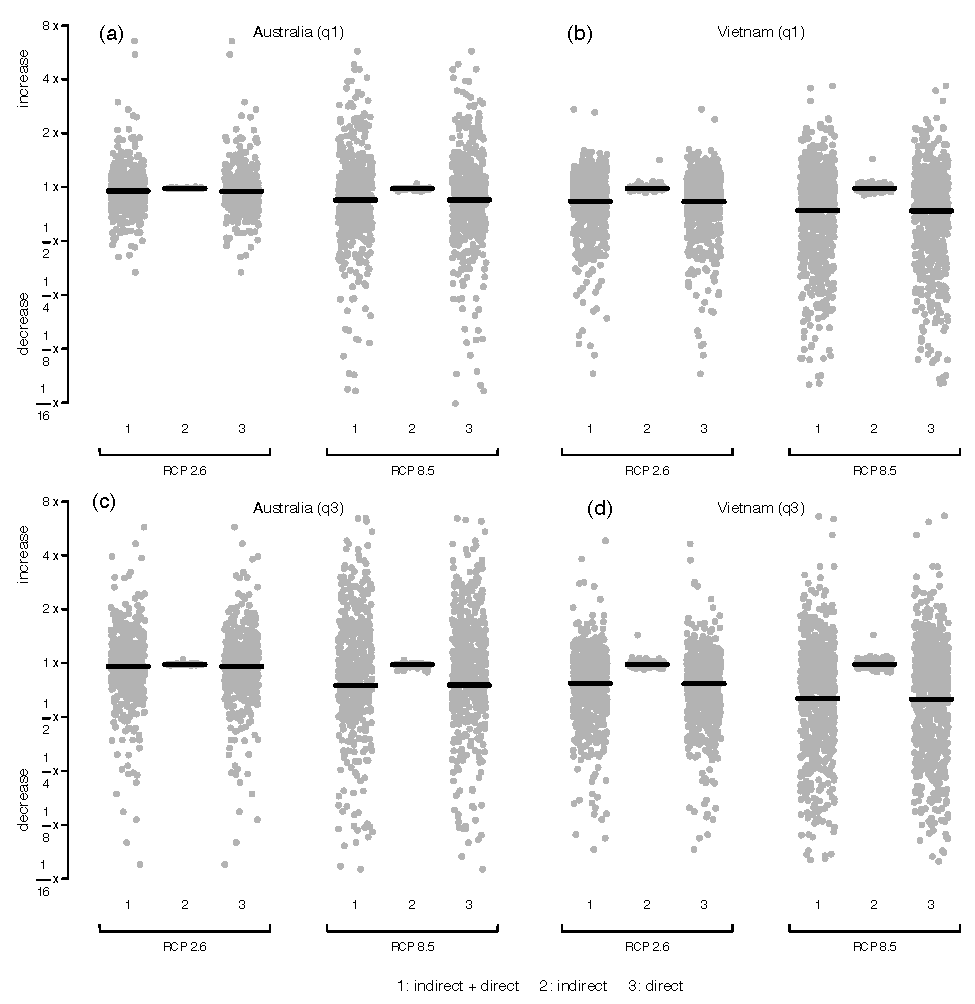
\includegraphics[width=\textwidth]{chapters/figures/chapter2/supfig1.pdf}
  \caption{Predicted change in mean potential habitat in Australia (a and c) and Vietnam (b and d) under the first quartile of GCMs (a and c) and the third quartile of GCMs (c and d). Main results are predictions under the cell-level medians. Plots are constrained on the y-axis to  $<$ 8x and $>$ 1/16 x for visual clarity. Figure created in R version 3.5.1 (https://www.R-project.org/) \citep{r_development_core_team_r_2008}.}
  \label{apx:ch2:fig1}
\end{figure*}

\begin{figure*}[htb]
  \centering
  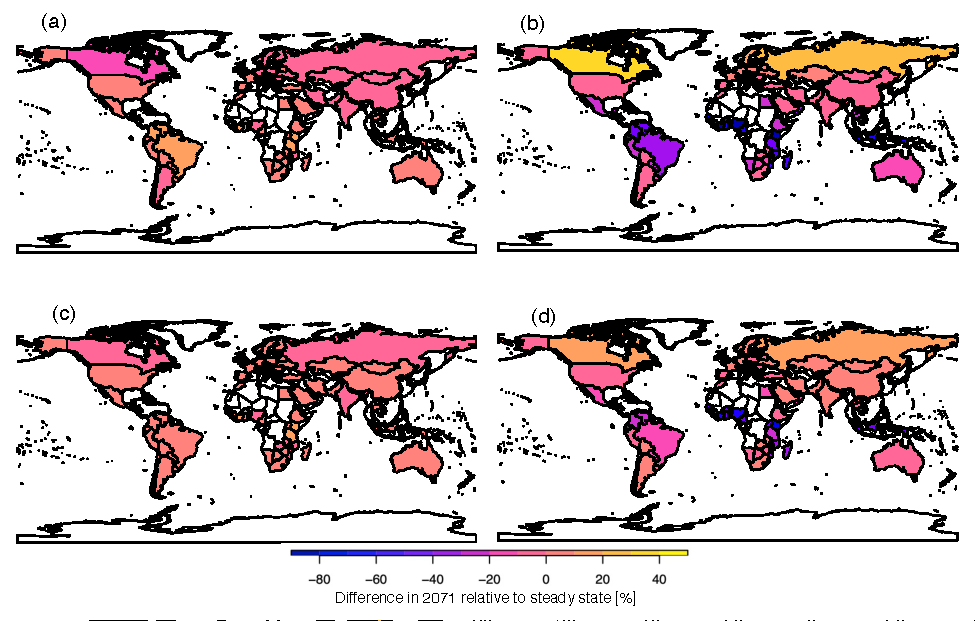
\includegraphics[width=\textwidth]{chapters/figures/chapter2/supfig2.pdf}
  \caption{Relative changes in total wheat sector outputs (a, b) and land endowments (c, d) of GTAP 9 countries under RCP 2.6 (a, c) and RCP 8.5 (b, d). The \% changes are relative to the economy after a forward propagation of the current economy without any scenario assumptions. Figure created in R version 3.5.1 (https://www.R-project.org/) \citep{r_development_core_team_r_2008}.}
  \label{apx:ch2:fig2}
\end{figure*}

\begin{table}[htb]
\centering
\caption{List of Global Circulation Models (GCM). Downscaled outputs from these models were used to estimate cell-level medians and first and third quartiles of cell-level predictions of 19 biolcim variables. Data are available through WorldClim \citep{hijmans_worldclim_nodate}.}
\label{apx:ch2:tab2}
\begin{tabularx}{\textwidth}{@{}l Y@{}}
\toprule
GCM & Source \\ \toprule
BCC-CSM1-1 & Beijing Climate Center, China Meteorological Administration \\
CCSM4 & University of Miami - RSMAS \\
CNRM-CM5 & Centre National de Recherches Météorologiques / Centre Européen de Recherche et Formation Avancée en Calcul Scientifique \\
GFDL-CM3 & NOAA Geophysical Fluid Dynamics Laboratory \\
GFDL-ESM2G & NOAA Geophysical Fluid Dynamics Laboratory \\
GISS-E2-R & NASA Goddard Institute for Space Studies \\
HadGEM2-AO & Met Office Hadley Centre (additional HadGEM2-ES realizations contributed by Instituto Nacional de Pesquisas Espaciais) \\
HadGEM2-ES & Met Office Hadley Centre (additional HadGEM2-ES realizations contributed by Instituto Nacional de Pesquisas Espaciais) \\
IPSL-CM5A-LR & Institut Pierre-Simon Laplace \\
MIROC-ESM-CHEM & Japan Agency for Marine-Earth Science and Technology, Atmosphere and Ocean Research Institute (The University of Tokyo), and National Institute for Environmental Studies \\
MIROC-ESM & Japan Agency for Marine-Earth Science and Technology, Atmosphere and Ocean Research Institute (The University of Tokyo), and National Institute for Environmental Studies \\
MIROC5 & Atmosphere and Ocean Research Institute (The University of Tokyo), National Institute for Environmental Studies, and Japan Agency for Marine-Earth Science and Technology \\
MPI-ESM-LR & Max-Planck-Institut für Meteorologie \\
MRI-CGCM3 & Meteorological Research Institute \\
NorESM1-M & Norwegian Climate Centre \\ \toprule
\end{tabularx}
\end{table}

\begin{table}[htb]
\centering
\caption{Relative contributions of commodity sectors to the total area harvested in 2016 13. These values inform the weight of predicted land endowment changes when estimating total changes to crop land area.}
\label{apx:ch2:tab3}
\begin{tabularx}{0.5\textwidth}{@{}llcc@{}}
\toprule
Sector & Full name & Australia & Vietnam \\ \bottomrule
c\_b & sugar cane, sugar beet & 0.020 & 0.018 \\
gro & cereal grains & 0.250 & 0.081 \\
ocr & crops nec & 0.094 & 0.129 \\
osd & oil seeds & 0.108 & 0.034 \\
pdr & paddy rice & 0.001 & 0.544 \\
pfb & plant-based fibres & 0.012 & 0.001 \\
v\_f & vegetables, fruit, nuts & 0.019 & 0.193 \\
wht & wheat & 0.496 & - \\ \bottomrule
\end{tabularx}
\end{table}

\begin{figure}[htb]
\centering
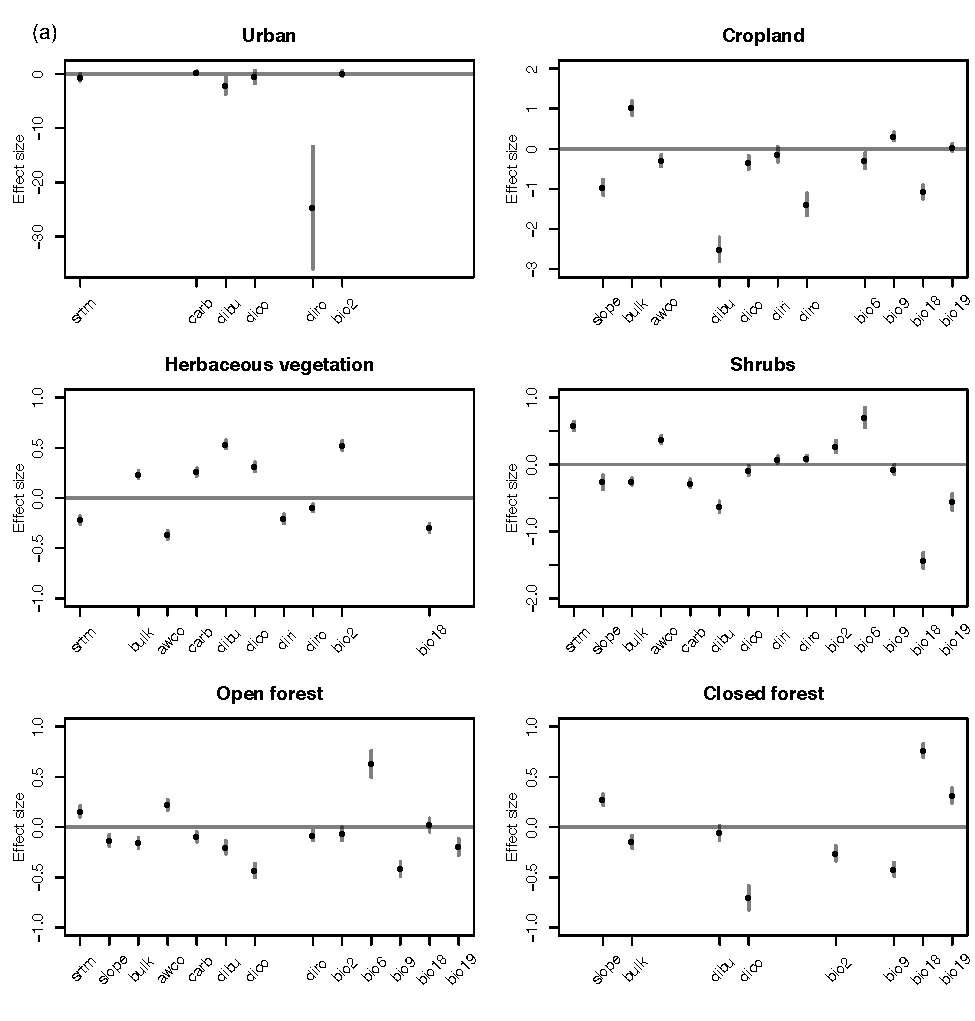
\includegraphics[width=1\linewidth]{chapters/figures/chapter2/supfig3a.pdf}
\label{apx:ch2:fig3}
\caption{}
\end{figure}

\begin{figure}[htb]
\continuedfloat
\centering
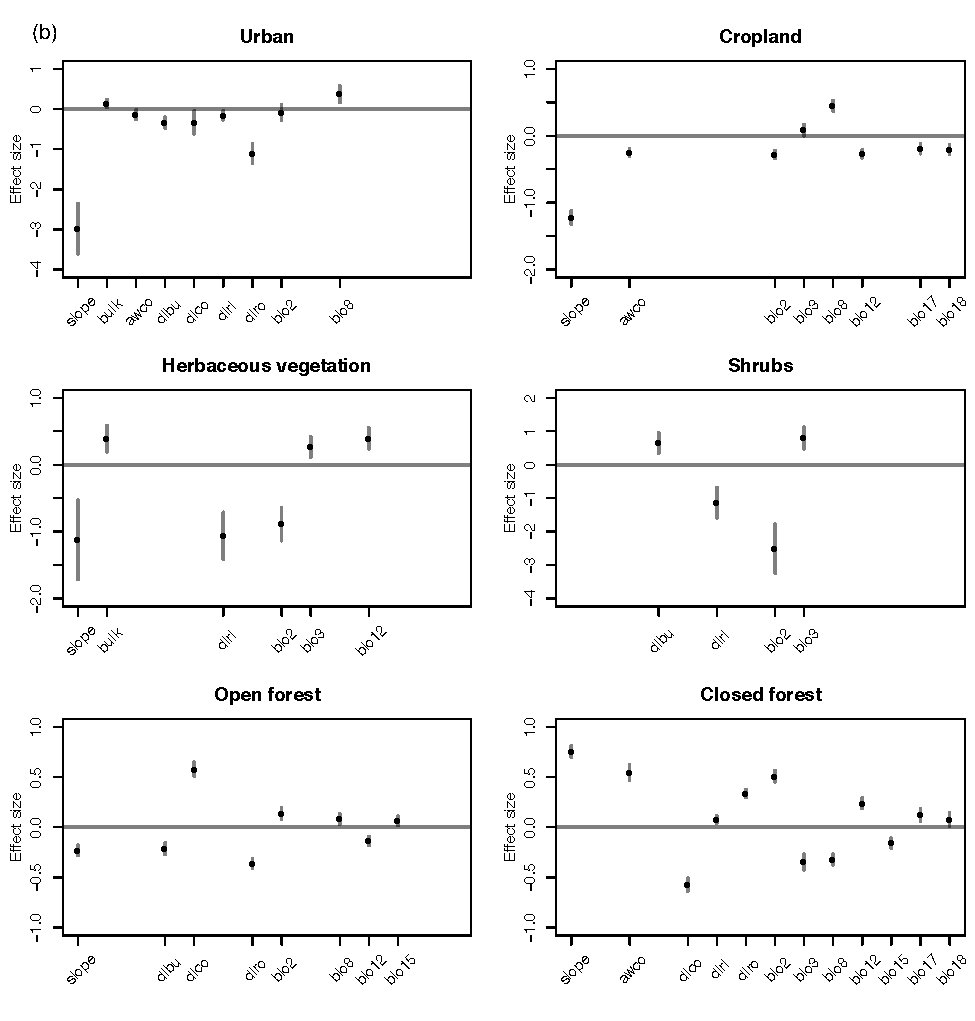
\includegraphics[width=1\linewidth]{chapters/figures/chapter2/supfig3b.pdf}
\caption{Effect sizes of predictors in land use suitability models. (a) Effect sizes of predictors in Australia and (b), effect sizes of predictors in Vietnam. Predictors were standardised and we used cross-validated Lasso penalization for predictor selection. Error bars are indicated in grey. The sample size for model building was n $=$ 20,000 in both countries. Figure created in R version 3.5.1 (https://www.R-project.org/) \citep{r_development_core_team_r_2008}.}
\end{figure}%

\begin{table}[htb]
\centering
\caption{Transition matrix of land use model. 1 indicate possible transitions from the class of the row to the class of the column of the cell. 0 indicate when transitions are not possible.}
\label{apx:ch2:tab4}
\begin{tabularx}{0.8\textwidth}{@{}lcccccc@{}}
\toprule
Class & Urban & Cropland & Herbaceous & Shrubs & Open Forest & Closed Forest \\ \bottomrule
Urban & 1 & 0 & 0 & 0 & 0 & 0 \\
Cropland & 1 & 1 & 1 & 1 & 1 & 1 \\
Herbaceous & 1 & 1 & 1 & 1 & 1 & 1 \\
Shrubs & 1 & 1 & 1 & 1 & 1 & 1 \\
Open Forest & 1 & 1 & 1 & 1 & 1 & 1 \\
Closed Forest & 1 & 1 & 1 & 1 & 1 & 1 \\ \bottomrule
\end{tabularx}
\end{table}

\chapter{Supplementary Information Chapter 3}\label{apx:ch3}

The multinomial model we used to estimate and predict land use suitability predicted very small probabilities of occurrence even in areas where a land use was not observed, because we were unable to capture all processes leading to the complete absence of a land use in an area. To capture some of these processes and prevent the unrealistic dispersal of land uses through the landscape (for example tiny fractions of urban land in the middle of forest), we applied a constraint that controlled the allocation of changes in land demand into areas where the land use has historically not occurred, thus ensuring patterns of clustering we also observed in the validation time series. However, it would be similarly unrealistic to prevent the new establishment of a land use type on each cell where the land use was not historically observed. Therefore, we parametrized the constraint by determining for each observed time step how many of the cells in which a land use type was observed were not occupied by that land use type in the preceding time step, expressed as a percentage of cells for each land use type. Since these percentages varied between time steps, we used the long-term average of the percentages (from the entire time series) to estimate the constraint parameter. During the simulation, we only allowed the estimated percentage of cells to go from being completely devoid in a land use to containing that land use in the next time step. This is similar to the elasticity parameter applied in the CLUE model series. The elasticities in CLUE are estimated based on expert knowledge or survey data and control the amount of shifting through the landscape a land use can experience between time steps without net changes to the overall amount of land under the land use type \citep{verburg_modeling_2002}. Our constraint controls shifting of a land use into cells completely devoid of that land use, but it does not control the shifting of land between cells that both contain the land use. As long as demand for a land use at the study area level prescribes changes in supply and a land use is allowed to decrease in any given area (we did not allow reductions in urban land to reflect the high initial investment), such shifts between cells already occupied by the land use are allowed.

\chapter{Supplementary Information Chapter 4}\label{apx:ch4}

\begin{table}[htb]
\centering
\caption{Aggregation of world regions in this study. We aggregated 140 GTAP 9 regions to 30 new regions to reduce the complexity of our GTAP INT model.}
\label{apx:ch4:gtapaggr}
\begin{tabularx}{\textwidth}{llY}
\toprule
Code 30 & Name 30 & Name (code) 140 \\
\bottomrule
aus & Australia & Australia (aus) \\
bra & Brazil & Brazil (aus) \\
can & Canada & Canada (can) \\
chn & China & China (chn) \\
deu & Germany & Germany (deu) \\
e25 & Rest of EU25 & Austria (aut), Belgium (bel), Cyprus (cyp), Czech Republic (cze), Denmark (dnk), Spain (esp), Estonia (est), Finland (fin), Greece (grc), Hungary (hun), Ireland (irl), Italy (ita), Lithuania (ltu), Luxemburg (lux), Latvia (lva), Malta (mlt), Netherlands (nld), Poland (pol), Portugal (prt), Slovakia (svk), Slovenia (svn), Sweden (swe) \\
fra & France & France (fra) \\
gbr & United Kingdom & United Kingdom (gbr) \\
idn & Indonesia & Indonesia (idn) \\
ind & India & India (ind) \\
jpn & Japan & Japan (jpn) \\
kor & Korea & Korea (kor) \\
mex & Mexico & Mexiko (mex) \\
mys & Malaysia & Malaysia (mys) \\
phl & Philippines & Philippines (phl) \\
rus & Russian Federation & Russian Federation (rus) \\
ssa & Sub-Saharan Africa & Benin (ben), Burkina Faso (bfa), Botswana (bwa), Cote d'Ivoire (civ), Cameroon (cmr), Ethiopia (eth), Ghana (gha), Guinea (gin), Kenya (ken), Madagascar (mdg), Mozambique (moz), Mauritius (mus), Malawi (mwi), Namibia (nam), Nigeria (nga), Rwanda (rwa), Senegal (sen), Togo (tgo), Tanzania (tza), Uganda (uga), South Central Africa (xac), Central Africa (xcf), Rest of Eastern Africa (xec), Rest of South African Customs (xsc), Rest of Western Africa (xwf), South Africa (zaf), Zambia (zmb), Zimbabwe (zwe) \\
tha & Thailand & Thailand (tha) \\
usa & United States of America & United States of America (usa) \\
vnm & Vietnam & Viet Nam (vnm) \\
xea & Rest of East Asia & Hong Kong (hkg), Mongolia (mng), Taiwan (twn), Rest of Asia (xea) \\
xer & Rest of Europe & Albania (alb), Bulgaria (bgr), Belarus (blr), Switzerland (che), Croatia (hrv), Norway (nor), Romania (rou), Ukraine (ukr), Rest of Eastern Europe (xee), Rest of EFTA (xef), Rest of Europe (xer) \\
xnf & North Africa & Egypt (egy), Morocco (mar), Tunisia (tun), Rest of North Africa (xnf) \\
xoc & Rest of Oceania & New Zealand (nzl), Rest of Oce \\
xsa & Rest of South Asia & Bangladesh (bgd), Sri Lanka (lka), Nepal (npl), Pakistan (pak), Rest of South Asia (xsa) \\
xse & Rest of Southeast Asia & Brunei Darassalam (brn), Cambodia (khm), Lao People's Democratic Republic (lao), Singapore (sgp), Rest of Southeast Asia (xse) \\
xsm & Rest of South America & Argentina (arg), Bolivia (bol), Chile (chl), Colombia (col), Ecuador (ecu), Peru (per), Paraguay (pry), Uruguay (ury), Venezuela (ven), Rest of South America (xsm) \\
xsu & Rest of Former Soviet Union & Kazakhstan (kaz), Kyrgyztan (kgz), Rest of Former Soviet Union (xsu) \\
xtw & Rest of the World & Costa Rica (cri), Domenican Republic (dom), Guatemala (gtm), Honduras (hnd), Jamaica (jam), Nicaragua (nic), Panama (pan), Puerto Rico (pri), El Salvador (slv), Trinidad and Tobago (tto), Rest of Central America (xca), Caribbean (xcb), Rest of North AMerica (xna), Rest of the World (xtw) \\
xws & Rest of Western Asia & United Arab Emirates (are), Armenia (arm), Azerbaijan (aze), Bahrain (bhr), Georgia (geo), Iran Islamic Republic of (irn), Israel (isr), Jordhan (jor), Kuwait (kwt), Oman (omn), Qatar (qat), Saudi Arabia (sau), Turkey (tur), Rest of Western Asia (xws) \\
\bottomrule
\end{tabularx}
\end{table}

\begin{figure*}[htb]
  \centering
    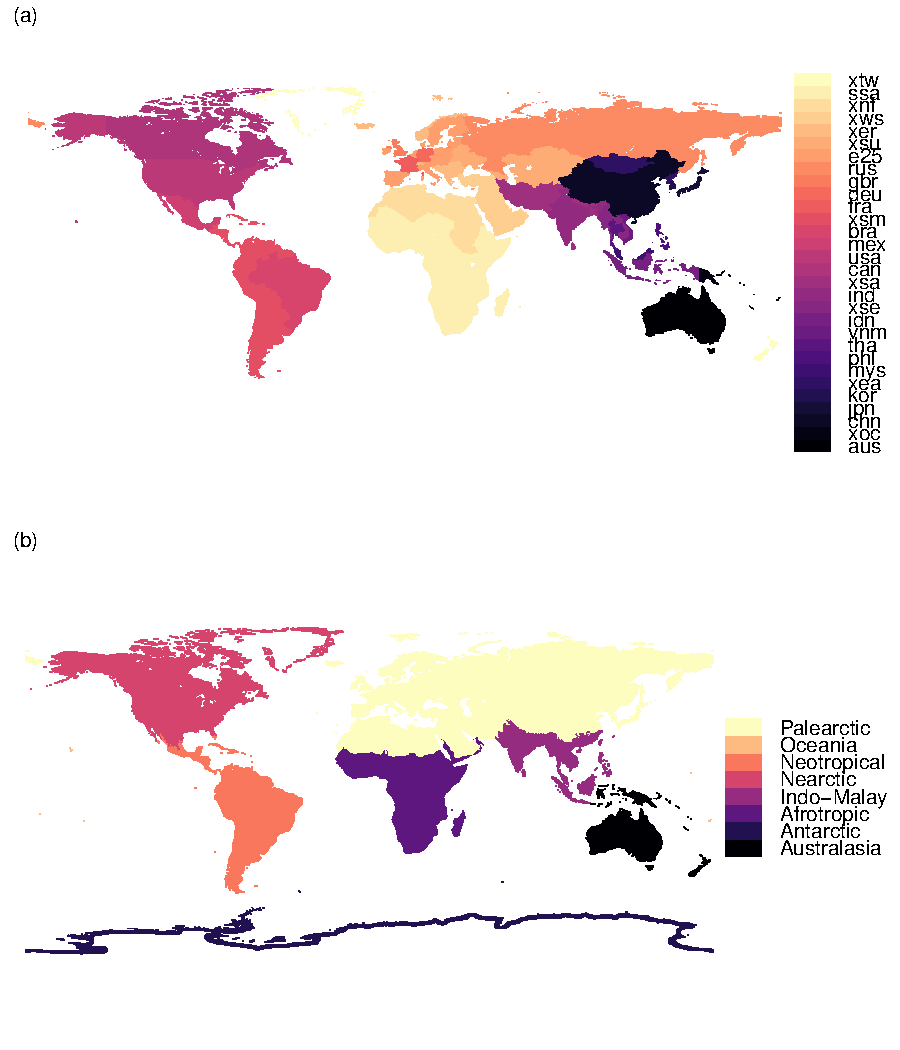
\includegraphics[width=1\linewidth]{chapters/figures/chapter4/fig_regionmap.pdf} 
    \caption{Maps of aggregations used in this study. (a) Regional aggregation of the GTAP INT model into 30 regions (see \Cref{apx:ch4:gtapaggr} for the countries belonging to each region). GTAP INT predictions and land-use predictions under SSP2 and SSP5 were made using this aggregation. (b) Bioegeographic realms used to aggregate biodiversity outcomes. Map adopted from \citet{olson2001terrestrial}.}
    \label{ch4:fig_regionmap}
\end{figure*}


\begin{table}[htb]
\centering
\caption{Relative contributions of commodity sectors to the total area harvested in 2019. These values inform the weight of predicted land endowment changes when estimating total changes to crop land area. c\_b: sugar cane, sugar beet; gro: Cereal grains nec; ocr: Crops nec; osd: oil seeds; pdr: paddy rice; pfb: plant-based fibres; v\_f: vegetables, fruit, nuts; wht: wheat.}
\label{apx:ch4:tab_faoharvested}
\begin{tabularx}{0.7\textwidth}{lllllllll}
\toprule
region & c\_b & gro & ocr & osd & pdr & pfb & v\_f & wht \\
\bottomrule
aus & 2.01 & 28.34 & 7.7 & 10.18 & 0.04 & 1.41 & 2.16 & 48.17 \\
xoc & 2.63 & 0.41 & 2.08 & 14.97 & 0.26 & 8.43 & 71.21 & 0.01 \\
chn & 0.92 & 23.82 & 2.3 & 11.93 & 16.26 & 4.49 & 27.35 & 12.94 \\
jpn & 0.74 & 2.14 & 1.62 & 5.25 & 53.33 & 3.37 & 26.24 & 7.32 \\
kor & 2.16 & 4.19 & 3.41 & 4.34 & 49.89 & 0.17 & 35.56 & 0.27 \\
xea & NA & 24.59 & 15.37 & 5.4 & 15.44 & 0.65 & 27.18 & 11.37 \\
mys & 2.14 & 0.1 & 0.29 & 84.96 & 9.23 & 0.22 & 3.06 & NA \\
phl & 2.63 & 16.75 & 0.71 & 2.11 & 30.95 & 0.21 & 46.64 & NA \\
tha & 8.94 & 5.61 & 1.39 & 20.72 & 47.3 & 0.15 & 15.88 & 0.01 \\
vnm & 1.68 & 7.14 & 4.21 & 6.83 & 53.73 & 0.84 & 25.57 & NA \\
idn & 0.94 & 13.54 & 2.28 & 41.15 & 22.55 & 3.62 & 15.92 & NA \\
xse & 1.04 & 5.49 & 23.34 & 9.62 & 45.79 & 1.14 & 13.33 & 0.25 \\
ind & 2.6 & 11.07 & 15.11 & 11.92 & 21.88 & 8.38 & 14.39 & 14.65 \\
xsa & 2.19 & 10.88 & 4.52 & 3.1 & 28.1 & 4.91 & 14.19 & 32.11 \\
can & 0.02 & 18.41 & 11.64 & 36.72 & NA & 0.04 & 1.3 & 31.86 \\
usa & 0.39 & 38.25 & 1.43 & 34.09 & 1.05 & 5.44 & 3.55 & 15.81 \\
mex & 5.27 & 55.19 & 9.49 & 2.26 & 0.25 & 1.74 & 21.96 & 3.84 \\
bra & 12.52 & 23.8 & 4.56 & 44.92 & 2.1 & 2.72 & 6.8 & 2.58 \\
xsm & 3.53 & 22.5 & 4.33 & 37.64 & 4.1 & 2.36 & 15.42 & 10.12 \\
fra & 0.08 & 29.16 & 2.42 & 15.01 & 0.11 & 3.29 & 11.27 & 38.66 \\
deu & 0.06 & 38.49 & 2 & 10.8 & 0 & 4.84 & 6.84 & 36.96 \\
gbr & NA & 31.33 & 4.02 & 12.43 & NA & 2.44 & 8.8 & 40.98 \\
rus & 0.11 & 23.6 & 3.42 & 21.97 & 0.3 & 1.8 & 5.14 & 43.66 \\
e25 & 0.39 & 33.35 & 2.44 & 18.56 & 0.76 & 1.37 & 17.55 & 25.58 \\
xsu & 0.07 & 24.71 & 2.22 & 21.16 & 0.63 & 4.02 & 9.07 & 38.12 \\
xer & 0.09 & 35.5 & 1.67 & 24.38 & 0.28 & 0.52 & 11.76 & 25.78 \\
xws & 0.21 & 26.99 & 5.98 & 9.64 & 0.9 & 3.39 & 18.03 & 34.86 \\
xnf & 0.54 & 35.43 & 14.58 & 16.66 & 1.95 & 2.76 & 11.59 & 16.48 \\
ssa & 0.9 & 32.38 & 19.34 & 10.46 & 6.64 & 6.45 & 22.71 & 1.12 \\
xtw & 0.92 & 11.54 & 1.89 & 2.39 & 28.64 & 1.25 & 48.34 & 5.04 \\
\bottomrule
\end{tabularx}
\end{table}

\begin{table}[htb]
\centering
\caption{Mapping of Global Land Systems (GLS) classes with land use classes and intensity classes. Table adopted from \citet{newbold_global_2015}.}
\label{apx:ch4:tab_glsmapping}
\begin{tabularx}{1\textwidth}{Ylllll}
\toprule
Global Land Systems classification & Primary & Secondary & Cropland & Pasture & Urban \\
\bottomrule
Cropland, extensive with few livestock & NA & NA & minimal & light & NA \\
Cropland, extensive with bovines, goats \& sheep & NA & NA & minimal & intense & NA \\
Cropland, extensive with pigs \& poultry & NA & NA & minimal & intense & NA \\
Cropland, medium intensive with few livestock & NA & NA & light & light & NA \\
Cropland, medium intensive with bovines, goats \& sheep & NA & NA & light & intense & NA \\
Cropland, medium intensive with pigs \& poultry & NA & NA & light & intense & NA \\
Cropland, intensive with few livestock & NA & NA & intense & light & NA \\
Cropland, intensive with bovines, goats \& sheep & NA & NA & intense & intense & NA \\
Cropland, intensive with pigs \& poultry & NA & NA & intense & intense & NA \\
Mosaic cropland and grassland with bovines, goats and sheep & NA & NA & intense & intense & NA \\
Mosaic cropland and grassland with pigs \& poultry & NA & NA & intense & intense & NA \\
Mosaic cropland (extensive) and grassland with few livestock & NA & NA & minimal & light & NA \\
Mosaic cropland (medium intensive) and grassland with few livestock & NA & NA & light & light & NA \\
Mosaic cropland (intensive) and grassland with few livestock & NA & NA & intense & light & NA \\
Mosaic cropland and forest with pigs \& poultry & NA & NA & intense & intense & NA \\
Mosaic cropland (extensive) and forest with few livestock & NA & NA & minimal & light & NA \\
Mosaic cropland (medium intensive) and forest with few livestock & NA & NA & light & light & NA \\
Mosaic cropland (intensive) and forest with few livestock & NA & NA & intense & light & NA \\
Dense forest & minimal & minimal & NA & NA & NA \\
Open forest with few livestock & light & light & NA & light & NA \\
Open forest with pigs \& poultry & intense & intense & NA & intense & NA \\
Mosaic grassland and forest & minimal & minimal & NA & NA & NA \\
Mosaic grassland and bare & minimal & minimal & NA & NA & NA \\
Natural grassland & minimal & minimal & NA & NA & NA \\
Grassland with few livestock & NA & NA & NA & light & NA \\
Grassland with bovines, goats and sheep & NA & NA & NA & intense & NA \\
Bare & NA & NA & NA & NA & NA \\
Bare with few livestock & NA & NA & NA & light & NA \\
Peri-urban and villages & NA & NA & NA & NA & minimal \\
Urban & NA & NA & NA & NA & intense \\
\bottomrule
\end{tabularx}
\end{table}

\begin{landscape}
\begin{table}[htb]
\captionsetup{width=1.5\textwidth}
\centering
\caption{Description of land use types and intensities. Table adopted from \citet{newbold_global_2015} and originally based on \citet{hudson_predicts_2014}. In this study, we combined different secondary vegetation types into one class, because the applied land use model was unable to explicitly model succession between secondary vegetation stages. We also excluded plantation forest, as this class is not covered in the LUH1 land-use data set we used as input for modelling.}
\label{apx:ch4:tab_intensity}
\begin{tabularx}{1.5\textwidth}{YlYYY}
\toprule
Level 1 Land Use &
  Predominant Land use &
  Minimal use &
  Light use &
  Intense use \\
  \bottomrule
\makecell[lt]{No evidence of prior destruction \\ of the vegetation \\ \\ Recovering after destruction \\ of the vegetation} &
  \makecell[lt]{Primary Vegetation \\ \\ \\ Secondary Vegetation} & Any disturbances identified are very minor (e.g., a trail or path) or very limited in the scope of their effect (e.g., hunting of a particular species of limited ecological importance). & 
  One or more disturbances of moderate intensity (e.g., selective logging) or breadth of impact (e.g., bushmeat extraction), which are not severe enough to markedly change the nature of the ecosystem. Primary sites in suburban settings are at least Light use. &
  One or more disturbances that are severe enough to markedly change the nature of the ecosystem; this includes clear- felling of part of the site too recently for much recovery to have occurred. Primary sites in fully urban settings should be classed as Intense use. \\
Human use (agricultural) &
  Plantation forest &
  Extensively managed or mixed timber, fruit/coffee, oil-palm or rubber plantations in which native understorey and/or other native tree species are tolerated, which are not treated with pesticide or fertiliser, and which have not been recently (\textless 20 years) clear- felled. &
  Monoculture fruit/coffee/rubber plantations with limited pesticide input, or mixed species plantations with significant inputs. Monoculture timber plantations of mixed age with no recent (\textless 20 years) clear-felling. Monoculture oil-palm plantations with no recent (\textless 20 years) clear-felling. &
  Monoculture fruit/coffee/rubber plantations with significant pesticide input. Monoculture timber plantations with similarly aged trees or timber/oil-palm plantations with extensive recent (\textless 20 years) clear-felling. \\
 &
  Cropland &
  Low-intensity farms, typically with small fields, mixed crops, crop rotation, little or no inorganic fertiliser use, little or no pesticide use, little or no ploughing, little or no irrigation, little or no mechanisation. &
  Medium intensity farming, typically showing some but not many of the following: large fields, annual ploughing, inorganic fertiliser application, pesticide application, irrigation, no crop rotation, mechanisation, monoculture crop. Organic farms in developed countries often fall within this category, as may high- intensity farming in developing countries. &
  High-intensity monoculture farming, typically showing many of the following features: large fields, annual ploughing, inorganic fertiliser application, pesticide application, irrigation, mechanisation, no crop rotation. \\
 &
  Pasture &
  Pasture with minimal input of fertiliser and pesticide, and with low stock density (not high enough to cause significant disturbance or to stop regeneration of vegetation). &
  Pasture either with significant input of fertiliser or pesticide, or with high stock density (high enough to cause significant disturbance or to stop regeneration of vegetation). &
  Pasture with significant input of fertiliser or pesticide, and with high stock density (high enough to cause significant disturbance or to stop regeneration of vegetation). \\
Human use (urban) &
  Urban &
  Extensive managed green spaces; villages. &
  Suburban (e.g. gardens), or small managed or unmanaged green spaces in cities. &
  Fully urban with no significant green spaces.\\
  \bottomrule
\end{tabularx}
\end{table}
\end{landscape}


% Please add the following required packages to your document preamble:
% \usepackage{lscape}
\begin{table}[htb]
\centering
\caption{Fraction of cells ($\%$) chosen in each time step for the new establishment of land use types (chosen cells were completely devoid of that land use in the preceding time step). Values derived from observed time steps 1990-2005 \citep{hurtt_harmonization_2011}.}
\label{apx:ch4:tab_newest}
\begin{tabularx}{0.55\textwidth}{lllllY}
\toprule
region & cropland & pasture & primary & secondary & urban \\
\bottomrule
aus    & 0.000    & 0.000   & 0.000   & 0.000     & 1.193 \\
xoc    & 0.291    & 0.000   & 0.011   & 1.058     & 0.422 \\
chn    & 0.119    & 0.000   & 0.100   & 2.672     & 0.408 \\
jpn    & 0.000    & 0.000   & 0.000   & 0.000     & 0.000 \\
kor    & 0.518    & 0.000   & 0.003   & 1.044     & 0.139 \\
xea    & 0.411    & 0.000   & 0.005   & 0.125     & 0.520 \\
mys    & 0.000    & 0.000   & 0.000   & 0.321     & 0.064 \\
phl    & 0.499    & 0.000   & 0.056   & 0.438     & 0.137 \\
tha    & 0.243    & 0.000   & 0.004   & 0.413     & 0.226 \\
vnm    & 0.051    & 0.000   & 0.000   & 0.000     & 0.076 \\
idn    & 0.000    & 0.000   & 0.000   & 0.466     & 0.055 \\
xse    & 0.041    & 0.000   & 0.000   & 0.000     & 1.282 \\
ind    & 0.442    & 0.000   & 0.008   & 0.046     & 0.564 \\
xsa    & 1.639    & 0.000   & 0.000   & 0.341     & 0.199 \\
can    & 0.000    & 0.000   & 0.000   & 0.018     & 0.388 \\
usa    & 0.164    & 0.000   & 0.000   & 0.078     & 0.418 \\
mex    & 1.481    & 0.000   & 0.238   & 0.733     & 0.007 \\
bra    & 0.000    & 0.000   & 0.000   & 0.000     & 0.204 \\
xsm    & 0.000    & 0.000   & 0.000   & 0.196     & 0.980 \\
fra    & 0.124    & 0.000   & 0.000   & 0.000     & 0.321 \\
deu    & 0.317    & 0.000   & 0.005   & 0.034     & 0.790 \\
gbr    & 0.743    & 0.000   & 0.012   & 0.138     & 0.321 \\
rus    & 0.232    & 0.000   & 0.110   & 0.844     & 0.245 \\
e25    & 0.000    & 0.000   & 0.000   & 0.000     & 0.819 \\
xsu    & 3.041    & 0.000   & 0.026   & 0.137     & 0.077 \\
xer    & 0.417    & 0.000   & 0.417   & 0.000     & 0.052 \\
xws    & 0.000    & 0.000   & 0.000   & 3.717     & 0.040 \\
xnf    & 0.925    & 0.000   & 0.009   & 2.112     & 0.780 \\
ssa    & 0.057    & 0.000   & 0.000   & 0.000     & 0.115 \\
xtw    & 0.990    & 0.000   & 0.028   & 0.182     & 0.149 \\
\bottomrule
\end{tabularx}
\end{table}



\begin{figure*}[htb]
  \centering
    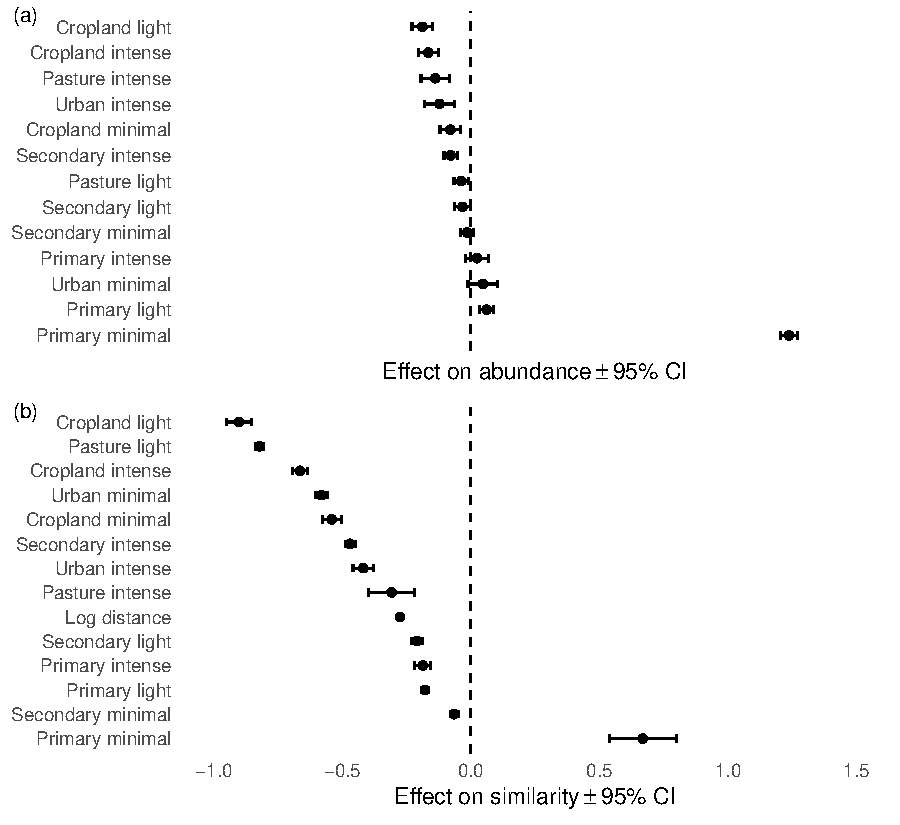
\includegraphics{chapters/figures/chapter4/fig_bdeffects.pdf} 
    \caption{Effects of land-use type/intensity on abundance (a) and compositional similarity (b). In the model of compositional similarity (b), listed land-use-related covariates are contrasts from primary minimal to each of the classes. In both models, we also applied a random effect to discount the effect of different studies.}
    \label{apx:ch4:fig_bdeffects}
\end{figure*}

\begin{figure*}[htb]
  \centering
    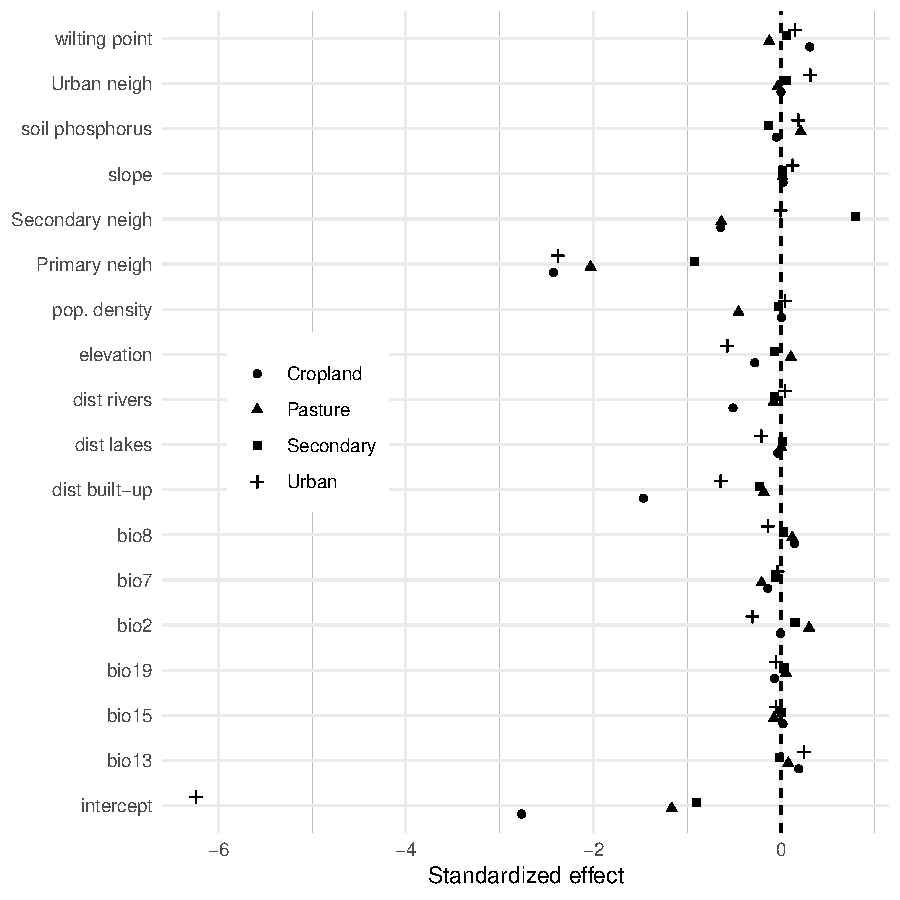
\includegraphics{chapters/figures/chapter4/fig_landuseeffects.pdf} 
    \caption{Standarized effects of socio-economic and biophysical drivers on global land-use suitability. We fitted one multinomial model for the entire world to obtain global effects for this figure. The reference class of the model was Primary (indicated by vertical dashed line through \(x=0\). All plotted effects are additive to this class. The effects of the intercepts for each class approximately reflect the initial share of each land-use type in the planet's land mass (prevalence). For example, the very small amount of Urban land at present is reflected in a strong negative intercept effect relative to Primary land. The fact that no intercept effect is positive relative to Primary land indicates that Primary land use has the highest prevalence.)}
    \label{apx:ch4:fig_landuseeffects}
\end{figure*}

    

\chapter{Links to \texttt{R} code}
\label{apx:ch5}
\newpage

\noindent All code accompanying this thesis is documented on GitHub. Permanently archived versions will be provided after the thesis has passed examination.


\section{Chapter 2}

\noindent Functions required for the analysis: \\
\textit{https://github.com/kapitzas/thesis\_ch2/blob/main/R/functions.R}
\vspace{0.3cm}

\noindent Preprocessing of environmental layers and presence data: \\
\textit{https://github.com/kapitzas/thesis\_ch2/blob/main/R/preprocessing.R}
\vspace{0.3cm}

\noindent Estimate future trajectories of land demand change from GTAP outputs: \\
\textit{https://github.com/kapitzas/thesis\_ch2/blob/main/R/gtaptrajectories.R}
\vspace{0.3cm}

\noindent Allocate land-use changes in line with demand trajectories in Dyna-CLUE: \\
\textit{https://github.com/kapitzas/thesis\_ch2/blob/main/R/landuse.R}
\vspace{0.3cm}

\noindent Build and predict MaxEnt SDM: \\
\textit{https://github.com/kapitzas/thesis\_ch2/blob/main/R/SDM.R}
\vspace{0.3cm}

\noindent Analysis of results and plots: \\
\textit{https://github.com/kapitzas/thesis\_ch2/blob/main/R/plots.R}
\vspace{0.3cm}

\section{Chapter 3}

\noindent Functions required for the analysis: \\
\textit{https://github.com/kapitzas/thesis\_ch3/blob/main/R/functions.R}
\vspace{0.3cm}

\noindent Preprocessing of layers: \\
\textit{https://github.com/kapitzas/thesis\_ch3/blob/main/R/preprocessing.R}
\vspace{0.3cm}

\noindent Land-use simulations using different model parametrizations: \\
\textit{https://github.com/kapitzas/thesis\_ch3/blob/main/R/simulation.R}
\vspace{0.3cm}

\noindent Analysis of results and plots: \\
\textit{https://github.com/kapitzas/thesis\_ch3/blob/main/R/results.R}
\vspace{0.3cm}
\newpage

\noindent \texttt{FLUTES} package: \texttt{devtools::install\_github("kapitzas/flutes")}\\
\noindent Detailed documentation for each function is built into the package. \\

\noindent Conversion of land-use fractions into integer representation, using multinomial draws: \\
\textit{https://github.com/kapitzas/flutes/blob/main/R/integerify.R}
\vspace{0.3cm}

\noindent Allocation of changes in land-use demand across the landscape: \\
\textit{https://github.com/kapitzas/flutes/blob/main/R/allocation.R}
\vspace{0.3cm}

\noindent Automatic reduction of a data set based on estimated correlations: \\
\textit{https://github.com/kapitzas/flutes/blob/main/R/correlations.R}
\vspace{0.3cm}

\noindent Extraction of observed land-use changes from a time series: \\
\textit{https://github.com/kapitzas/flutes/blob/main/R/demand.R}
\vspace{0.3cm}

\noindent Application of neighbourhood functions to data: \\
\textit{https://github.com/kapitzas/flutes/blob/main/R/neighbourhood.R}
\vspace{0.3cm}

\noindent Estimation of parameters of multinomial, multi-class land-use suitability model: \\
\textit{https://github.com/kapitzas/flutes/blob/main/R/suitmodel.R}
\vspace{0.3cm}

\section{Chapter 4}
\noindent Functions required for the analysis: \\
\textit{https://github.com/kapitzas/thesis\_ch4/blob/main/R/functions.R}
\vspace{0.3cm}

\noindent Preprocessing of layers: \\
\textit{https://github.com/kapitzas/thesis\_ch4/blob/main/R/preprocessing.R}
\vspace{0.3cm}

\noindent Estimate future trajectories of land demand change from GTAP outputs and Message 8.5 land-use data: \\
\textit{https://github.com/kapitzas/thesis\_ch4/blob/main/R/demands.R}
\vspace{0.3cm}

\noindent Land-use intensity model and prediction: \\
\textit{https://github.com/kapitzas/thesis\_ch4/blob/main/R/intensity\_model\_validation.R}
\vspace{0.3cm}

\noindent Allocation of land demand changes: \\
\textit{https://github.com/kapitzas/thesis\_ch4/blob/main/R/landuse.R}
\vspace{0.3cm}

\noindent Estimation and prediction of biodiversity intactness, based on PREDICTS: \\
\textit{https://github.com/kapitzas/thesis\_ch4/blob/main/R/BII.R}
\vspace{0.3cm}


\noindent Analysis of results and figures: \\
\textit{https://github.com/kapitzas/thesis\_ch4/blob/main/R/figures.R}
\vspace{0.3cm}


\section{Other \texttt{R} packages}
\noindent Further packages developed for this thesis were 

\begin{itemize}

\item \texttt{kapitzas/WorldClimTiles}, a package to download and merge tiled worldclim data at 30 arcsec resolution (required in \Cref{ch2})
\item \texttt{kapitzas/gdaltools}, a package to link R directly with the \texttt{gdal} library for fast spatial processing, developed by Saras Windecker and Casey Visintin \citep{windecker_gdaltools_2021} and adjusted for this thesis (required in \Cref{ch3,ch4}).
\end{itemize}

% \renewcommand{\thesection}{2.1.\arabic{section}}

%---------------------------------------------------------- 
% BACK
% list of symbols / references / index etc
%---------------------------------------------------------- 
%\backmatter
%
%\chapter{List of Symbols}
%
%
%The following list is neither exhaustive nor exclusive, but may be helpful.
%\begin{list}{}{%
%\setlength{\labelwidth}{24mm}
%\setlength{\leftmargin}{35mm}}
%\item[$a$, $b$, $c$, $d$\dotfill] annihilation operators
%\item[$a^\dagger$, $b^\dagger$, $c^\dagger$, $d^\dagger$\dotfill] creation
%operators
%\end{list}

\end{document}
